\chapterimage{tabl_cont4.pdf} % Chapter heading image

\chapter{Qlik}
\begin{comment}
    FARE PROCESSAMENTO DEL DATASET -> UNIONE DATASET
\end{comment}


\begin{comment}
!!!PRECISARE CHE NEL SECONDO DATASET L'ANNO ARRIVA FINO AL 2019
SCREENSHOT GENERALI PER TUTTE LE DASHBOARD SENZA FILTRI
    1 - Dashboard 1 -> Analisi della Variazione della Temperatura Media nel Mondo (no filtri)
        1.1 Variazione temperatura media 1965 (più freddo)
        1.2 Variazione temperatura media 2020 (più caldo)
        1.3 Variazione temperatura media Italia
    2 - Dashboard 2 -> Variazione temperatura media Mondo
        2.1 -> filtri 1960 (spiegazione Russia)
        2.2 -> filtri 2000-2010-2020
        Scrivere cazzate sul riscaldamento globale per spiegare i cinque stati in classifica
    3 - Dashboard 3 -> Mappa Variazione temperatura media nel mondo (immagini vicine)
        3.1 Italia (2000)
        3.2 Italia (2019)
        3.3 Cina (2000)  
        3.4 Cina (2019)
        3.5 USA (2000)
        3.6 USA (2019)
        3.7 India (2000)
        3.8 India (2019)

    4 - Dashboard 4 -> Emissioni Co2 
        4.1 2000
        4.2 2010
        4.3 2019
    5 - Dashboard 5 -> Energie rinnovabili
        5.1 2000 
        5.2 2010
        5.3 2019 
        5.4 Cina (2000-2010-2019) ->accenni economici
        5.5 Stati Uniti (2000-2010-2019) 
    6 - Dashboard 6 -> confronto CO2 e rinnovabile (->confronti tra i valori)
        6.1 Cina 
        6.2 Stati Uniti
        6.3 Italia -> abbiamo abbassato la Co2 senza dare contributi (->questioni politiche economiche)
Quando c'è scritto (2000-2010-2019) sono tre screen!
\end{comment}


%RISCRIVERE TUTTO
\section{Introduzione}
%Cos'è Qlik ->Qlik Sense e View (slide di Bonifazi). Funzionamento e caricamento dei dati (compresi i tipi di file che si possono inserire)

\textbf{Qlik} è una delle principali aziende nel settore della Business Intelligence (BI) e dell'analisi dei dati, fondata nel 1993 a Lund, in Svezia, e attualmente con sede negli Stati Uniti, in Pennsylvania. L'azienda si distingue per la sua innovativa tecnologia di analisi dei dati, che permette agli utenti di esplorare, visualizzare e comprendere le informazioni in modo dinamico e intuitivo.

\begin{figure}[h!]
    \centering
    
\includegraphics[width=0.4\linewidth]{capitolo_1/img1/QlikLogo.pdf}
    \caption{Qlik - Logo}
    \label{fig:QlikLogo}
\end{figure}

Il primo prodotto di successo di Qlik è stato \textbf{QlikView}, una soluzione che ha rivoluzionato la BI orientata all'utente. QlikView è una piattaforma di \textit{Guided Analytics} che permette alle aziende di sviluppare applicazioni interattive con dashboard, grafici e visualizzazioni avanzate. Tuttavia, gli utenti finali possono solo esplorare i dati senza poter modificare o personalizzare l’applicazione, poiché la creazione e la gestione sono affidate a sviluppatori e analisti.

Successivamente, l'azienda ha sviluppato \textbf{Qlik Sense}, una piattaforma avanzata di \textit{Self-Service Analytics} che consente agli utenti di analizzare i dati in autonomia, creando report personalizzati e dashboard interattive.

Uno degli elementi distintivi di Qlik è il suo motore associativo, che si differenzia dai tradizionali sistemi query-based. Questo motore permette di elaborare calcoli e aggregazioni in tempo reale, evidenziando le relazioni tra i dati senza limitazioni imposte da una struttura rigida di query \textit{SQL}\footnote{Contrariamente a Qlik, la maggior parte degli strumenti di BI odierni si fonda su database relazionali e adotta un approccio basato su query, il che può risultare limitante. Infatti, \textit{SQL} non è stato progettato per supportare analisi interattive dei dati, restringendo le opportunità di esplorazione dinamica.}. Tale approccio consente di:

\vspace{2mm}
\begin{itemize}
    \item Integrare e combinare dati provenienti da fonti eterogenee senza perdita di informazioni;
    
    \item Favorire un'esplorazione dei dati intuitiva e flessibile da parte di utenti di ogni livello;
    
    \item Eliminare i tempi di attesa tipici del ciclo \textit{ask, wait, answer} dei sistemi tradizionali;
\end{itemize}
\vspace{2mm}

In Qlik Sense, i dati vengono organizzati all'interno di applicazioni (\textbf{app}), che rappresentano ambienti strutturati per l'analisi, comprendenti misure, dimensioni, visualizzazioni e fogli di lavoro. I \textbf{fogli}, a loro volta, permettono di organizzare le informazioni in base agli obiettivi analitici, facilitando la costruzione di una panoramica chiara e dettagliata delle metriche chiave.


\noindent Il caricamento dei dati in Qlik Sense può avvenire attraverso diversi metodi:

\vspace{2mm}
\begin{itemize}
    \item \textbf{Catalogo dati}, che consente di integrare dati aziendali e di terze parti;
    
    \item \textbf{Caricamento da file e sorgenti esterne}, che permette di importare dati da file locali o unità di rete in diversi formati (\texttt{CSV}, \texttt{Excel}, \texttt{XML}, \texttt{HTML}, ecc.);
    
    \item \textbf{Editor di caricamento dati}, che offre funzionalità avanzate per la manipolazione dei dati attraverso script personalizzati;
\end{itemize}
\vspace{2mm}

%Magari fare anche un'unica subsection chiamata "Caricamento dei dati" o "del dataset" se risulta più comodo
\subsection{Caricamento dei dati}

Il caricamento dei dati in Qlik è stato realizzato sfruttando il \textbf{motore associativo}, una delle caratteristiche più potenti di questo software, che consente di collegare automaticamente i dati provenienti da diverse fonti senza dover definire manualmente le relazioni tra le tabelle. Questo approccio permette di esplorare le informazioni in modo più dinamico e flessibile, consentendo di individuare correlazioni significative tra le variabili. Nel nostro caso, abbiamo utilizzato tre files principali: FAOSTAT\_data\_1-10-2022, Global Data on Sustainable Energy (2000-2020) e FAOSTAT\_data\_11-24-2020. Il primo contiene informazioni relative ai cambiamenti di temperatura nei diversi paesi nel corso degli anni, il secondo raccoglie dati sulle emissioni di CO\textsubscript{2}, la produzione di energia elettrica e altri indicatori legati alla sostenibilità energetica, mentre il terzo fornisce dettagli specifici sui paesi, tra cui i codici identificativi come \texttt{ISO2 Code} e \texttt{Country Code}, fondamentali per l’integrazione con gli altri dataset e per la realizzazione di visualizzazioni cartografiche basate sulle mappe geografiche.

Prima di caricare i dati in Qlik, è stato necessario effettuare un processo di \textbf{pulizia e uniformazione}, per garantire la corretta integrazione delle informazioni provenienti dalle diverse fonti. Un aspetto critico di questa fase è stata l’uniformazione dei nomi dei paesi, dal momento che ogni dataset poteva adottare convenzioni di denominazione differenti. Per evitare problemi di associazione e garantire la coerenza dei dati, è stato necessario un intervento manuale per rendere i nomi dei paesi biunivoci, in modo che fossero identici in tutte le tabelle.

Una volta completata la fase di preparazione e pulizia dei dati, questi sono stati caricati in Qlik, che grazie al suo motore associativo ha identificato automaticamente le connessioni tra le tabelle. In particolare, il software ha riconosciuto i campi in comune come \texttt{Area}, \texttt{Country}, \texttt{Entity} e \texttt{Year}, stabilendo le relazioni tra i diversi dataset senza la necessità di creare query SQL per unire le informazioni in modo tradizionale. Questo ha reso l’analisi più fluida e intuitiva, consentendo di navigare tra i dati senza vincoli rigidi e di esplorare interattivamente le correlazioni tra le variabili.

Grazie a questa integrazione, è stato possibile realizzare diverse visualizzazioni avanzate. Inoltre, sfruttando il dataset FAOSTAT\_data\_11-24-2020, sono state realizzate mappe interattive, permettendo agli utenti di analizzare rapidamente le differenze geografiche. Un altro aspetto interessante dell’uso del motore associativo è la possibilità di effettuare filtraggi dinamici: selezionando un anno specifico, tutte le visualizzazioni si aggiornano automaticamente per mostrare solo i dati relativi a quel periodo, facilitando il confronto tra diverse fasi temporali. L’approccio adottato con Qlik ha, dunque, garantito una maggiore flessibilità nell’analisi. La capacità del motore associativo di stabilire relazioni tra i dati in modo automatico ha reso possibile un’esplorazione più approfondita e interattiva, migliorando la precisione e la coerenza delle informazioni presentate nelle dashboard. Questo ha permesso di sviluppare un sistema di analisi efficace e dettagliato, utile per comprendere le dinamiche legate all’energia, alle emissioni di CO\textsubscript{2} e ai cambiamenti climatici nei diversi paesi nel corso degli anni.

\section{Data Analysis}
%obiettivi delle analisi ed elenco delle dashboard da presentare
Per l'esecuzione delle analisi proposte, si è fatto ricorso alle \textbf{Dashboard}, strumenti avanzati per la visualizzazione e l'analisi dei dati. Attraverso l'impiego di grafici, indicatori e tabelle interattive, esse agevolano un'esplorazione strutturata delle informazioni, consentendo agli utenti di condurre indagini approfondite in linea con i propri obiettivi analitici.

\noindent Successivamente, saranno proposti i grafici e le analisi dedotte dalle seguenti Dashboard, estratte dai due dataset oggetto dell'analisi:
\vspace{2mm}
\begin{itemize}
    \item \textbf{Analisi della variazione della Temperatura Media (Visione Temporale)};
    \item \textbf{Analisi della Variazione della Temperatura Media nel Mondo (Visione Geografica)};
    \item \textbf{Confronto Globale sulle Variazioni della Temperatura Media};
    \item \textbf{Tendenze Climatiche e CO\textsubscript{2}};
    \item \textbf{Panorama dell’energia rinnovabile};
\end{itemize}
\vspace{2mm}

\subsection{Analisi della variazione della Temperatura Media (Visione Temporale)}
\label{Sezione_dash_1}
%Per ogni subsection mettere il titolo della analisi effettuata. Fare una piccola introduzione, mettere l'immagine generale e senza filtri. 
Per condurre l’analisi illustrata in Figura \ref{fig:dashboard_world}, è stato impiegato esclusivamente il dataset \textbf{FAOSTAT Temperature Change}. Questo studio si concentra sulla variazione della temperatura media registrata in diversi Paesi del mondo, con l’obiettivo di fornire un’analisi dettagliata e approfondita dei cambiamenti climatici nel tempo. L’approccio adottato permette di esaminare le tendenze globali e di individuare eventuali anomalie o fenomeni significativi, contribuendo così a una maggiore comprensione dell’impatto del riscaldamento globale su scala internazionale.

\begin{figure}[h!]
    \centering
    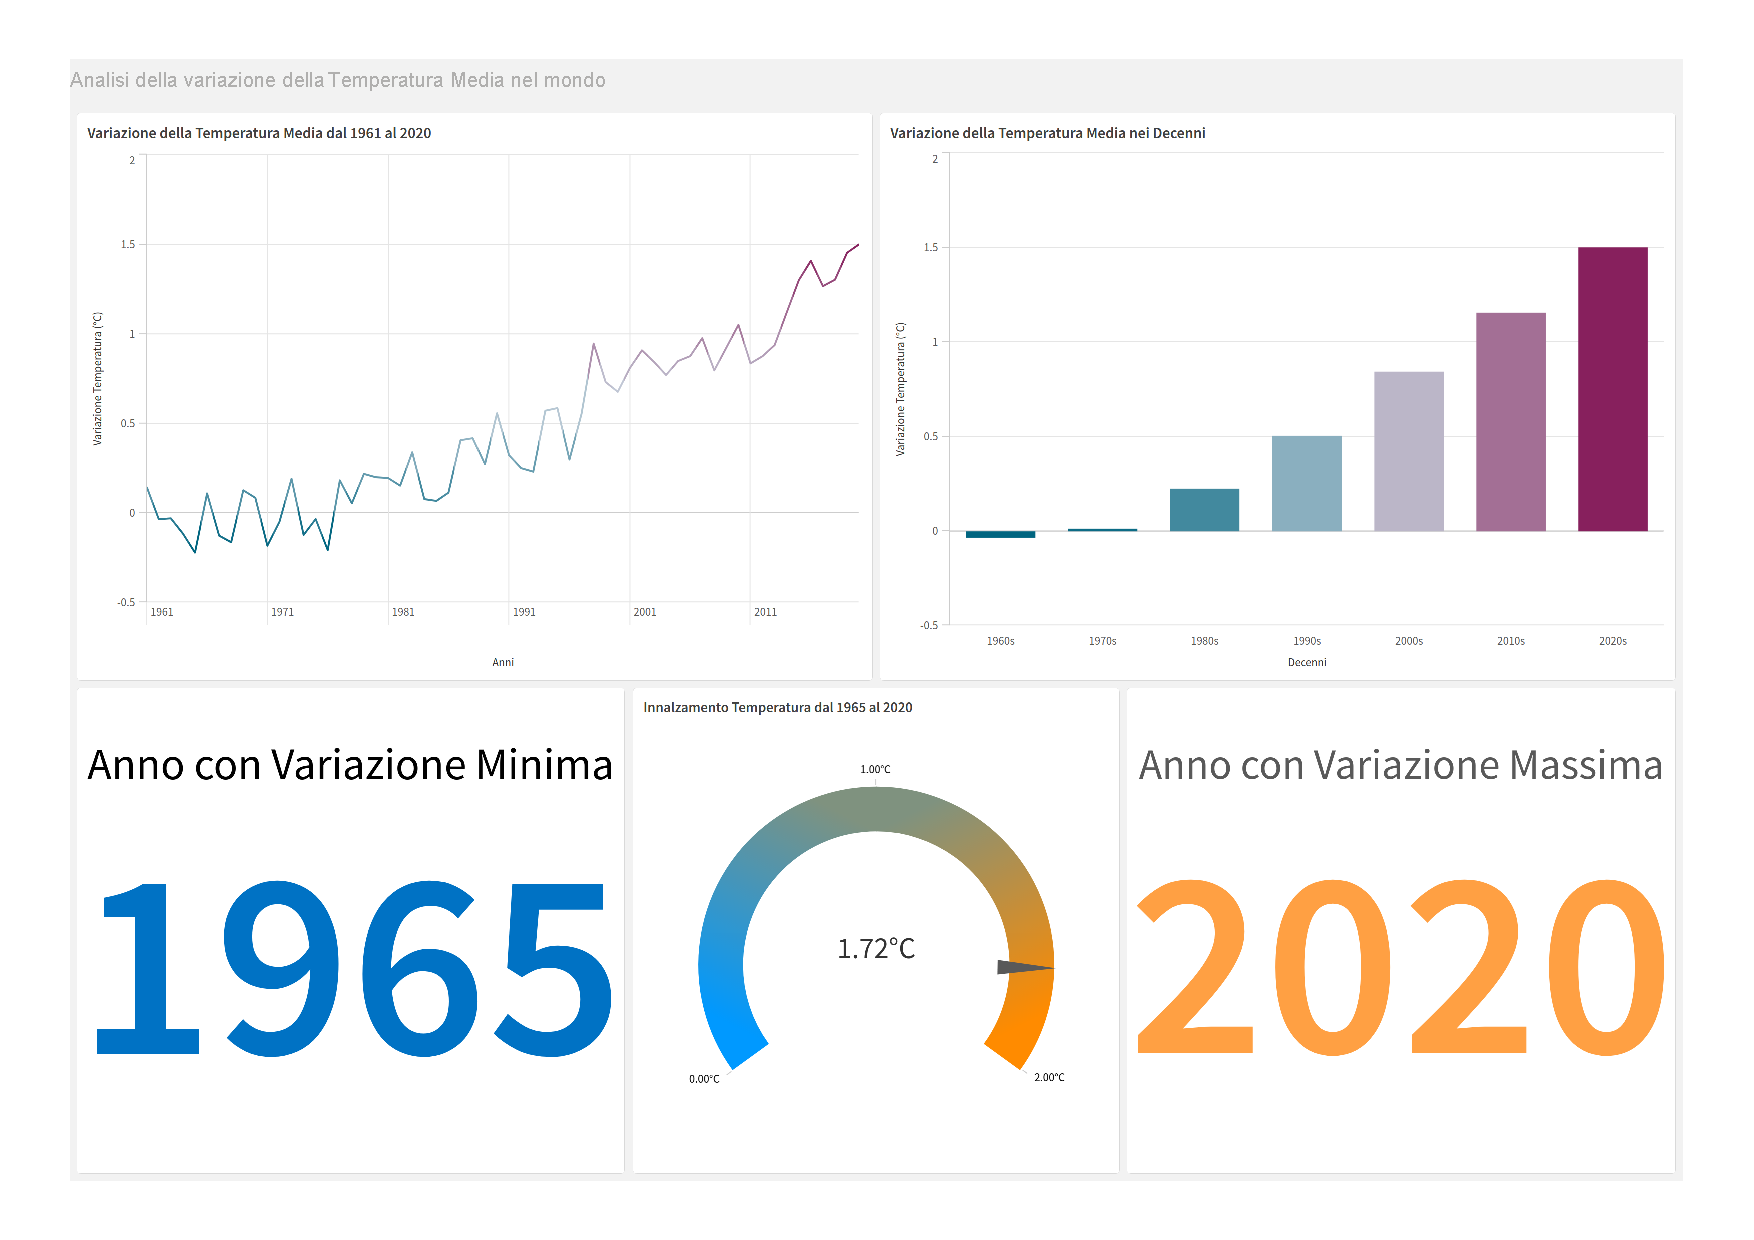
\includegraphics[width=0.98\linewidth]{capitolo_2/img2/1.0 Analisi della variazione della Temperatura Media nel mondo.pdf}
    \caption{Analisi della variazione della Temperatura Media (Visione Temporale)}
    \label{fig:dashboard_world}
\end{figure}

\subsubsection{Struttura Dashboard}
%spiegazione della struttura e dei grafici presenti
La struttura della Dashboard si articola attraverso diversi grafici e KPI\footnote{\textit{Key Performance Indicators} (\textit{KPI}) rappresenta un indicatore di prestazione, utilizzato per valutare le prestazioni nel tempo in relazione a un obiettivo specifico.}, consentendo una visione chiara e semplice delle condizioni del cambiamento climatico dal 1961 fino al 2020.

Nella parte superiore della Dashboard sono presenti due grafici principali, ognuno dei quali fornisce una prospettiva distinta sull'andamento delle temperature nel periodo analizzato. A sinistra, troviamo un grafico a linee intitolato \textbf{Variazione della Temperatura Media dal 1961 al 2020}, il quale visualizza in modo chiaro e continuo l'evoluzione della temperatura media nel corso degli anni compresi nel dataset. Questo grafico consente di osservare le fluttuazioni annuali e le tendenze generali di riscaldamento o raffreddamento nel tempo.

A destra, è invece presente un istogramma denominato \textbf{Variazione della Temperatura Media nei Decenni}, che offre una panoramica sull'andamento della temperatura nel corso dei diversi decenni. Questo grafico è particolarmente utile per comprendere come l'aumento della temperatura si sia manifestato in modo differenziato nel tempo, evidenziando gli anni o i decenni in cui il cambiamento sia stato più marcato. 

Nella parte inferiore della Dashboard sono visibili due indicatori chiave di performance (KPI), rispettivamente denominati \textbf{Anno con Variazione Minima} e \textbf{Anno con Variazione Massima}. Questi KPI sono strettamente correlati all'ultimo grafico presente nella sezione, intitolato \textbf{Innalzamento della Temperatura dal 1965 al 2020}, il quale funge da misuratore per visualizzare l'evoluzione della temperatura media nel corso del periodo indicato. I due KPI evidenziano, infatti, gli anni che presentano la più bassa e la più alta variazione di temperatura rispetto alla media del periodo, offrendo così una visione chiara dei valori estremi in relazione all'andamento complessivo. In particolare, l'analisi del grafico permette di evidenziare l'incremento medio della temperatura registrato tra i due anni estremi individuati dai KPI, fornendo un quadro completo e preciso delle fluttuazioni climatiche nel tempo. 

\subsubsection{Obiettivo dell'analisi}
%spiegazione di tutte le analisi facendo notazioni anche economiche e 
Questa Dashboard è stata progettata per fornire un'analisi dettagliata delle variazioni di temperatura media globali nel periodo che va dal 1961 al 2020. Il suo obiettivo principale è offrire una visione chiara e articolata dell'andamento delle temperature nel corso di sei decadi, mettendo in evidenza le tendenze di riscaldamento e raffreddamento che hanno caratterizzato il periodo analizzato. Attraverso una serie di grafici interattivi, tra cui un grafico a linee che illustra la variazione annuale della temperatura e un istogramma che evidenzia l'andamento decennale, la Dashboard consente agli utenti di comprendere facilmente l'intensità e la distribuzione delle variazioni termiche.

In particolare, l'analisi dei KPI, come l'indicazione dell'anno con la variazione minima e massima di temperatura, permette di identificare i periodi di maggiore e minore riscaldamento, rendendo possibile una valutazione dettagliata dei fenomeni di cambiamento climatico. 

Ad esempio, il grafico a linee intitolato \textbf{Variazione della Temperatura Media dal 1961 al 2020} mostra un chiaro trend di riscaldamento globale, con un'accelerazione significativa degli aumenti di temperatura negli ultimi decenni. Si osserva che, mentre nei primi anni del periodo considerato (1960-1980) le fluttuazioni annuali erano relativamente contenute, dal 1990 in poi la curva mostra un'impennata costante, particolarmente evidente dopo il 2000. Questo indica che, non solo la temperatura media globale è aumentata nel corso del tempo, ma l'intensità di tale aumento è notevolmente aumentata negli ultimi venti anni, segnalando un fenomeno di riscaldamento accelerato. L'istogramma \textbf{Variazione della Temperatura Media nei Decenni}, d'altra parte, offre una panoramica sull'andamento delle temperature suddiviso per decenni. Esaminando i dati decennali, si osserva che la variazione della temperatura media nei decenni 1981-1990 e 1991-2000 è stata piuttosto moderata, ma dal decennio 2001-2010 in poi, l'andamento mostra incrementi sempre più marcati. Ad esempio, il decennio 2011-2020 evidenzia l'aumento di temperatura più significativo di tutti, con un incremento che supera in modo consistente le medie storiche. Questo potrebbe essere correlato all'intensificazione dei fenomeni legati al cambiamento climatico, come ondate di calore, modifiche nei pattern meteorologici e scioglimento dei ghiacciai.

La Dashboard, grazie alla sua interattività e alla visualizzazione chiara dei dati, si rivela uno strumento estremamente utile per ricercatori, decisori politici e professionisti del settore ambientale. Essa fornisce loro le informazioni necessarie per analizzare il cambiamento climatico, pianificare politiche ambientali informate e monitorare l'efficacia delle azioni intraprese in risposta ai cambiamenti climatici. 

Infatti, questa Dashboard può essere adattata con il fine di fornire uno strumento utile all'analisi dell'andamento delle variazioni di temperatura media in specifiche aree geografiche. Ad esempio, come illustrato nella Figura \ref{fig:dashboard_italia}, è stato realizzato un adattamento dei grafici per analizzare i dati relativi all'Italia. 

\begin{figure}[h!]
    \centering
    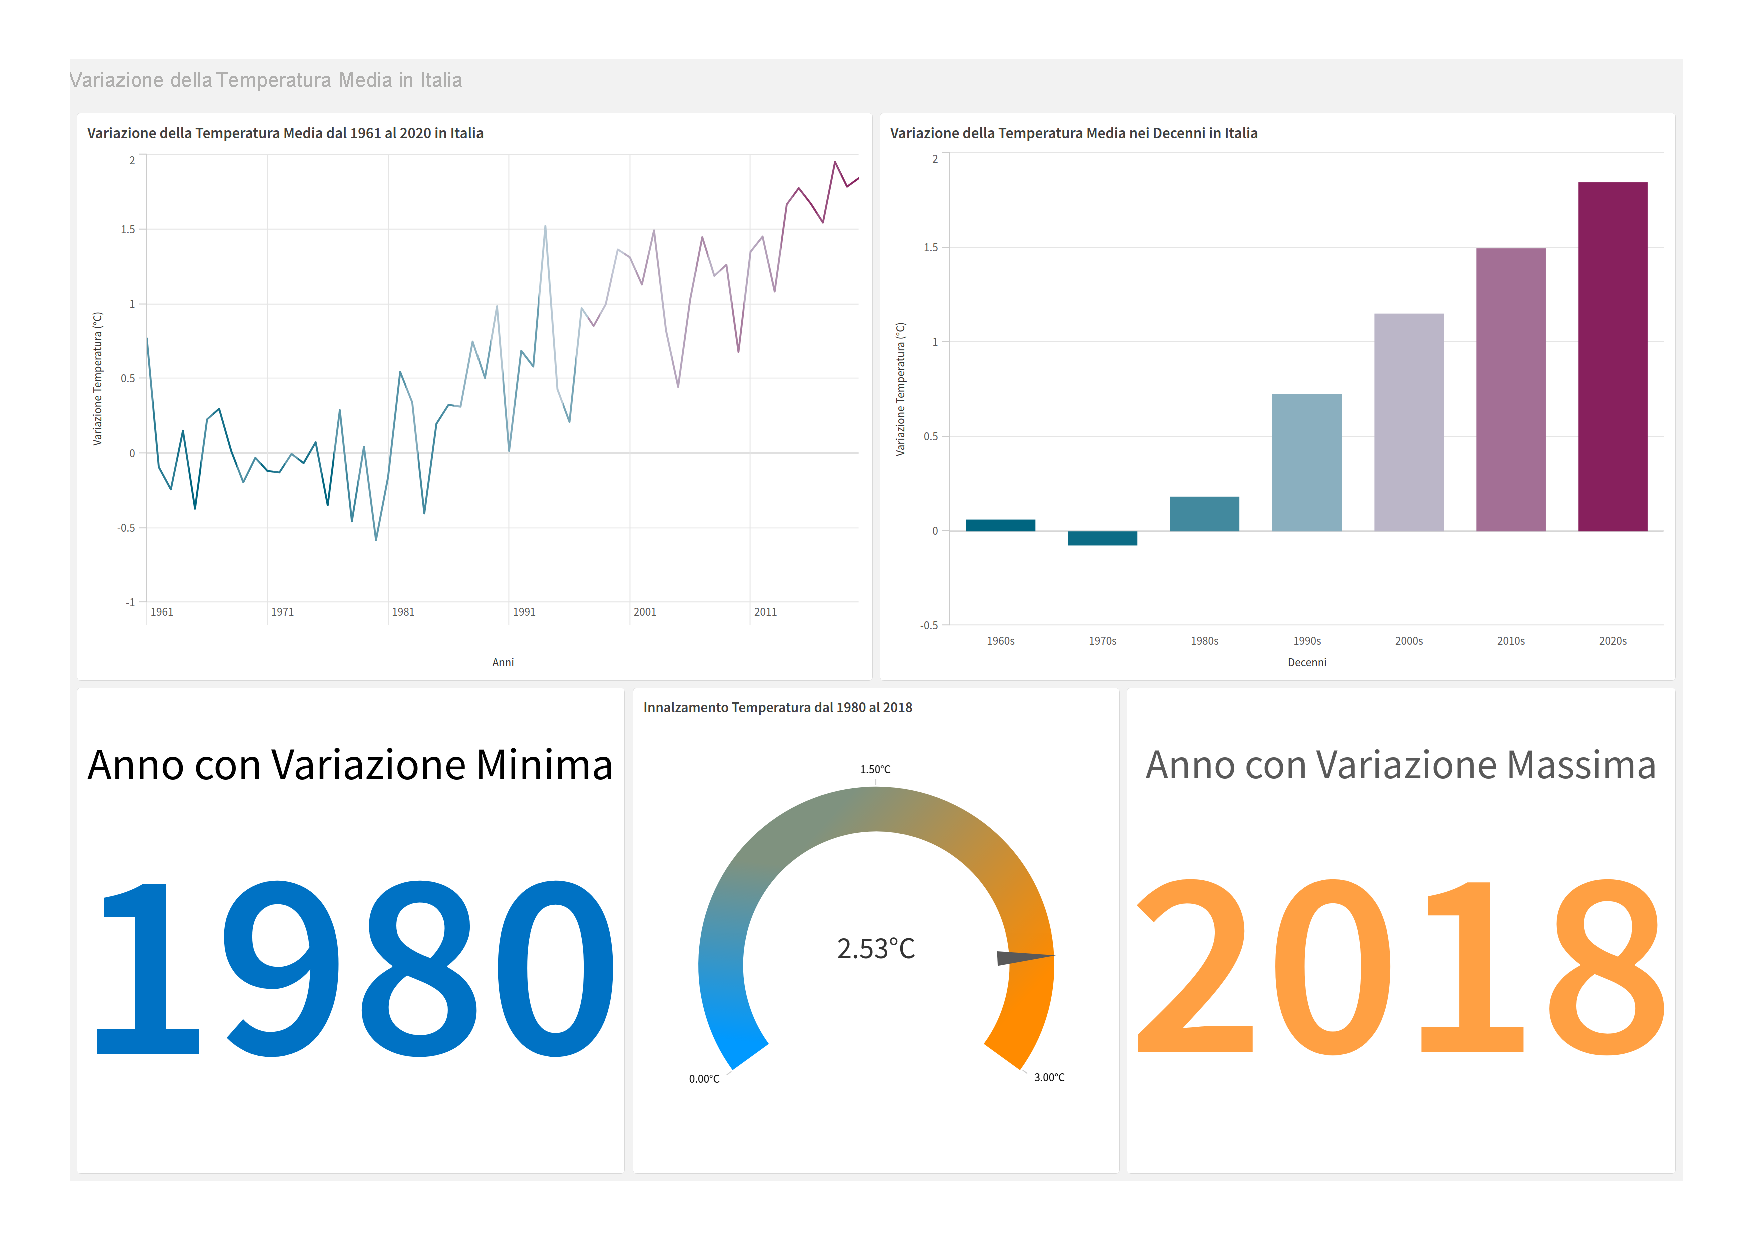
\includegraphics[width=0.98\linewidth]{capitolo_2/img2/1.3 Variazione temperatura media Italia.pdf}
    \caption {Variazione temperatura media Italia}
    \label{fig:dashboard_italia}
\end{figure}

Grazie a questa personalizzazione, è possibile monitorare in modo preciso e dettagliato le fluttuazioni termiche a livello nazionale, consentendo una valutazione più approfondita dei trend climatici nel contesto italiano. In questo modo è possibile confrontare le variazioni delle temperature medie con quelle internazionali, facilitando 
l'individuazione di eventuali anomalie o tendenze significative. Ad esempio, è possibile osservare come la variazione media della temperatura, rappresentata nel grafico \textbf{Innalzamento della Temperatura dal 1980 al 2020}, evidenzi le fluttuazioni termiche tra due anni che presentano i valori estremi, ovvero quelli con i picchi massimi e minimi di temperatura. Il dato riportato, \texttt{2.53°C}, risulta essere significativamente superiore alla media globale. In effetti, l'innalzamento delle temperature appare più marcato in Italia rispetto alla tendenza osservata negli altri paesi inclusi nell'analisi. Ciò suggerisce che l'Italia stia sperimentando un riscaldamento più rapido rispetto alla media internazionale, indicando potenziali anomalie climatiche locali.

\subsection{Analisi della Variazione della Temperatura Media nel Mondo (Visione Geografica)}

La Dashboard, illustrata in Figura \ref{fig:2.0}, è stata realizzata utilizzando esclusivamente il dataset \textbf{FAOSTAT Temperature Change}. Analogamente alla Dashboard presentata nella Sezione \ref{Sezione_dash_1}, questo studio si concentra sull'analisi delle variazioni della temperatura media a livello globale. L'unica differenza consiste nell'adozione di una visualizzazione geografica, che permette di osservare l'andamento delle temperature su base territoriale, anziché temporale. Questo approccio offre una panoramica più dettagliata delle fluttuazioni termiche nelle diverse regioni del mondo, facilitando il confronto tra aree geografiche e l'individuazione di tendenze climatiche specifiche.

\begin{figure}[h!]
    \centering
    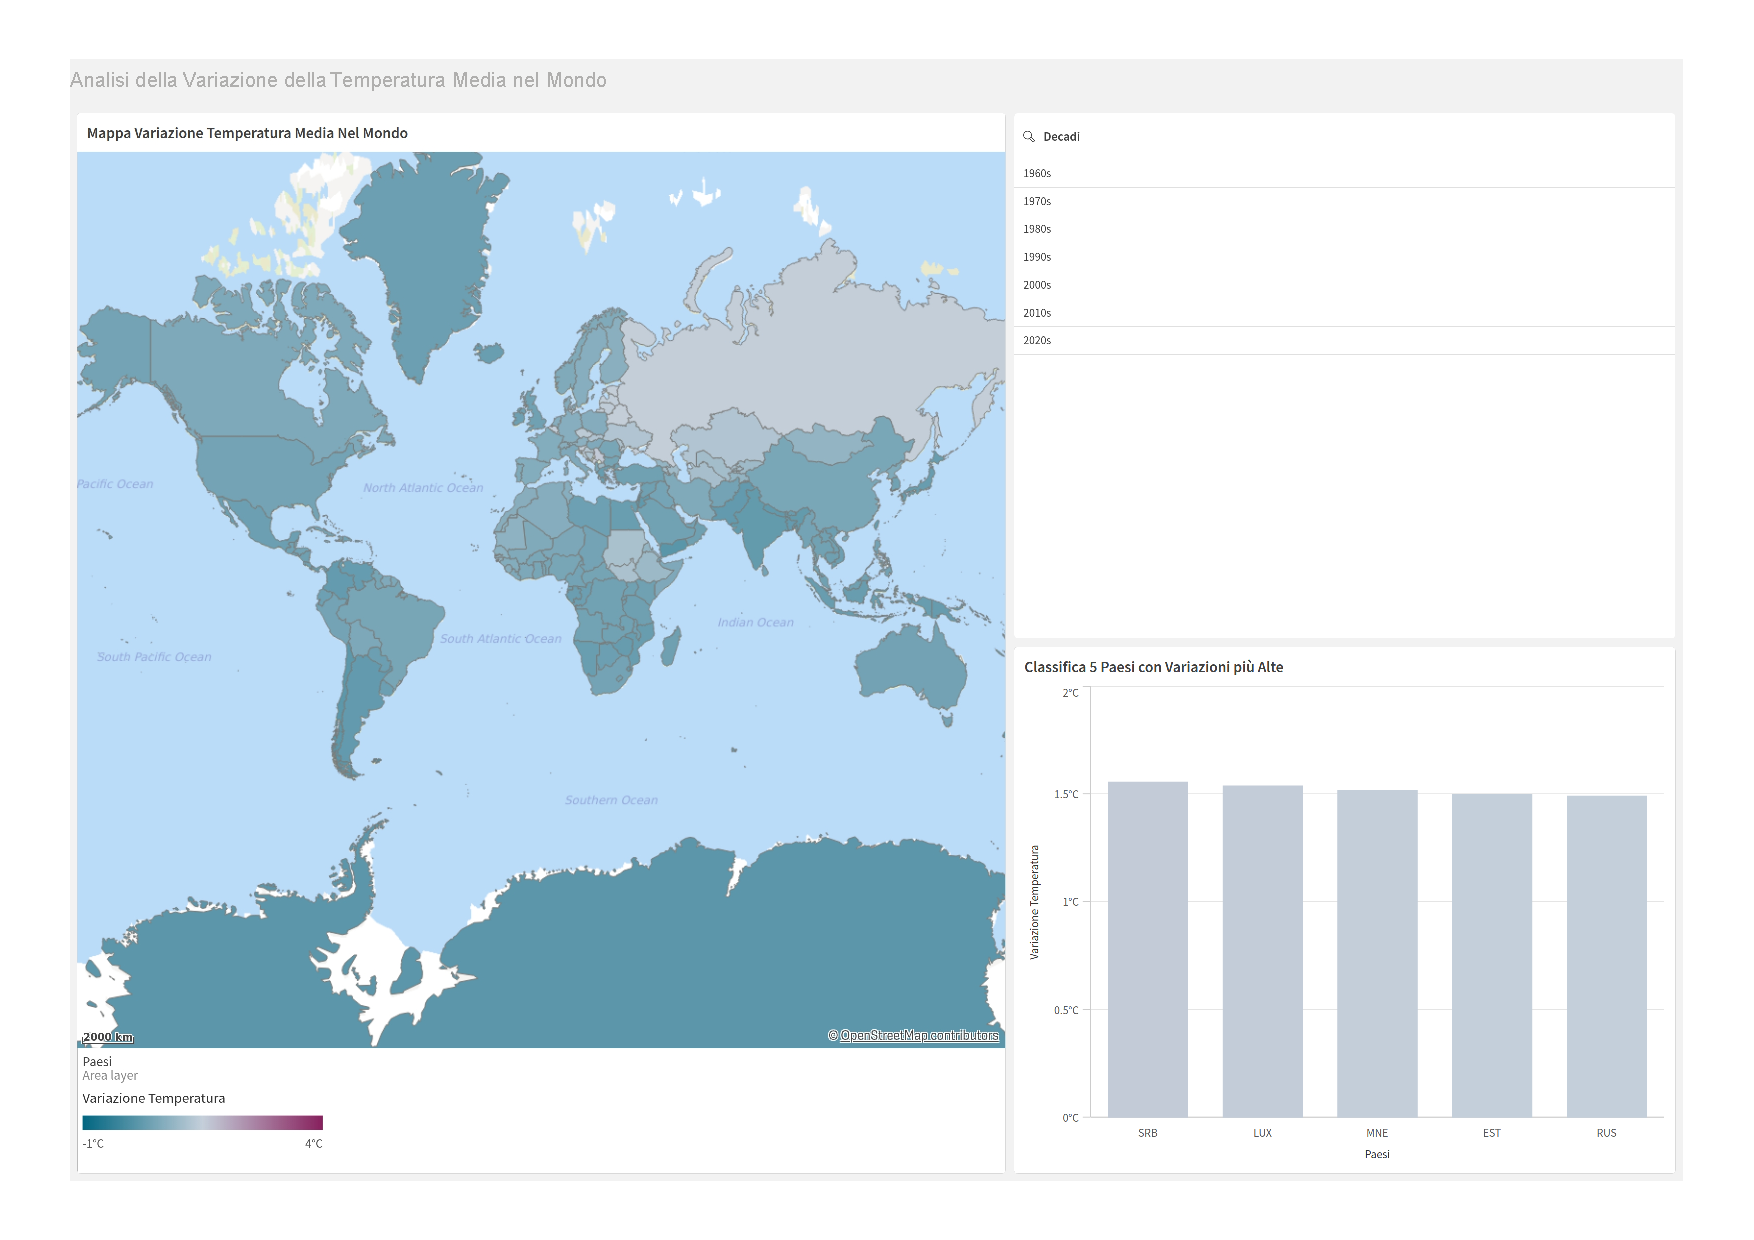
\includegraphics[width=0.98\linewidth]{capitolo_2/img2/2.0 Analisi della Variazione della Temperatura Media nel Mondo.pdf}
    \caption{Analisi della variazione della Temperatura Media nel Mondo (Visione Geografica)}
    \label{fig:2.0}
\end{figure}

\subsubsection{Struttura Dashboard}
La struttura della Dashboard è articolata in diverse sezioni, ognuna delle quali fornisce una rappresentazione grafica dell'andamento delle variazioni della temperatura media a livello globale nel periodo compreso tra il 1961 e il 2020.

Sulla sinistra della Dashboard è presente una visualizzazione geografica, denominata \textbf{Mappa della Variazione della Temperatura Media nel Mondo}, nella quale gli stati inclusi nell'analisi sono colorati in base alla variazione termica registrata. Questa mappa permette di osservare chiaramente le differenze geografiche nelle fluttuazioni di temperatura, evidenziando le aree con i cambiamenti più significativi.

Sulla destra della Dashboard, invece, è visibile un grafico denominato \textbf{Classifica dei 5 Paesi con le Variazioni più Alte}, che permette di identificare i cinque Paesi che hanno registrato la variazione più elevata della temperatura, sia in senso positivo che negativo, rispetto alla media globale. Inoltre, grazie all'implementazione di un filtro, è possibile selezionare la decade di interesse, consentendo così di eseguire analisi più mirate e dettagliate su specifici periodi temporali.

\subsubsection{Obiettivo dell'Analisi}
La principale finalità di questa Dashboard è fornire uno strumento interattivo e intuitivo per l'analisi delle variazioni della temperatura media globale nel periodo compreso tra il 1961 e il 2020. L'obiettivo è consentire agli utenti di esplorare in dettaglio l'andamento delle temperature nel tempo, sia a livello globale che per specifici paesi e regioni. La Dashboard permette di visualizzare in modo chiaro e immediato come la temperatura media sia cambiata in tutto il mondo, con particolare attenzione alle tendenze geografiche e temporali.

Una delle caratteristiche distintive della Dashboard è la capacità di offrire una visualizzazione geografica delle variazioni di temperatura media. Utilizzando la \textbf{Mappa della Variazione della Temperatura Media nel Mondo}, gli utenti possono esaminare i cambiamenti delle temperature a livello di singoli Stati. Ad esempio, è possibile osservare come alcune regioni, come il Circolo Polare Artico, abbiano registrato aumenti significativi della temperatura, mentre altre aree, come certe zone dell'Africa, abbiano mostrato variazioni più contenute. Questa rappresentazione geografica evidenzia le disparità nei cambiamenti climatici, facilitando l'identificazione delle aree più vulnerabili agli effetti del riscaldamento globale.

Inoltre, grazie al filtro temporale, gli utenti hanno la possibilità di selezionare periodi specifici di interesse per analizzare in dettaglio le decadi di cambiamento climatico. Ad esempio, selezionando la decade \texttt{1960s} (come illustrato in Figura \ref{fig:2.1}), si può osservare come le variazioni di temperatura fossero relativamente più uniformi e contenute rispetto a quelle registrate nelle decadi successive, come le \texttt{2000s-2010s-2020s}, in cui emerge un trend di crescita più marcato. Infatti, analizzando la mappa, si nota come i colori tendano a diventare progressivamente più violacei, indicando un aumento positivo della variazione di temperatura nel corso di questi ultimi decenni.

\begin{figure}[h!]
    \centering
    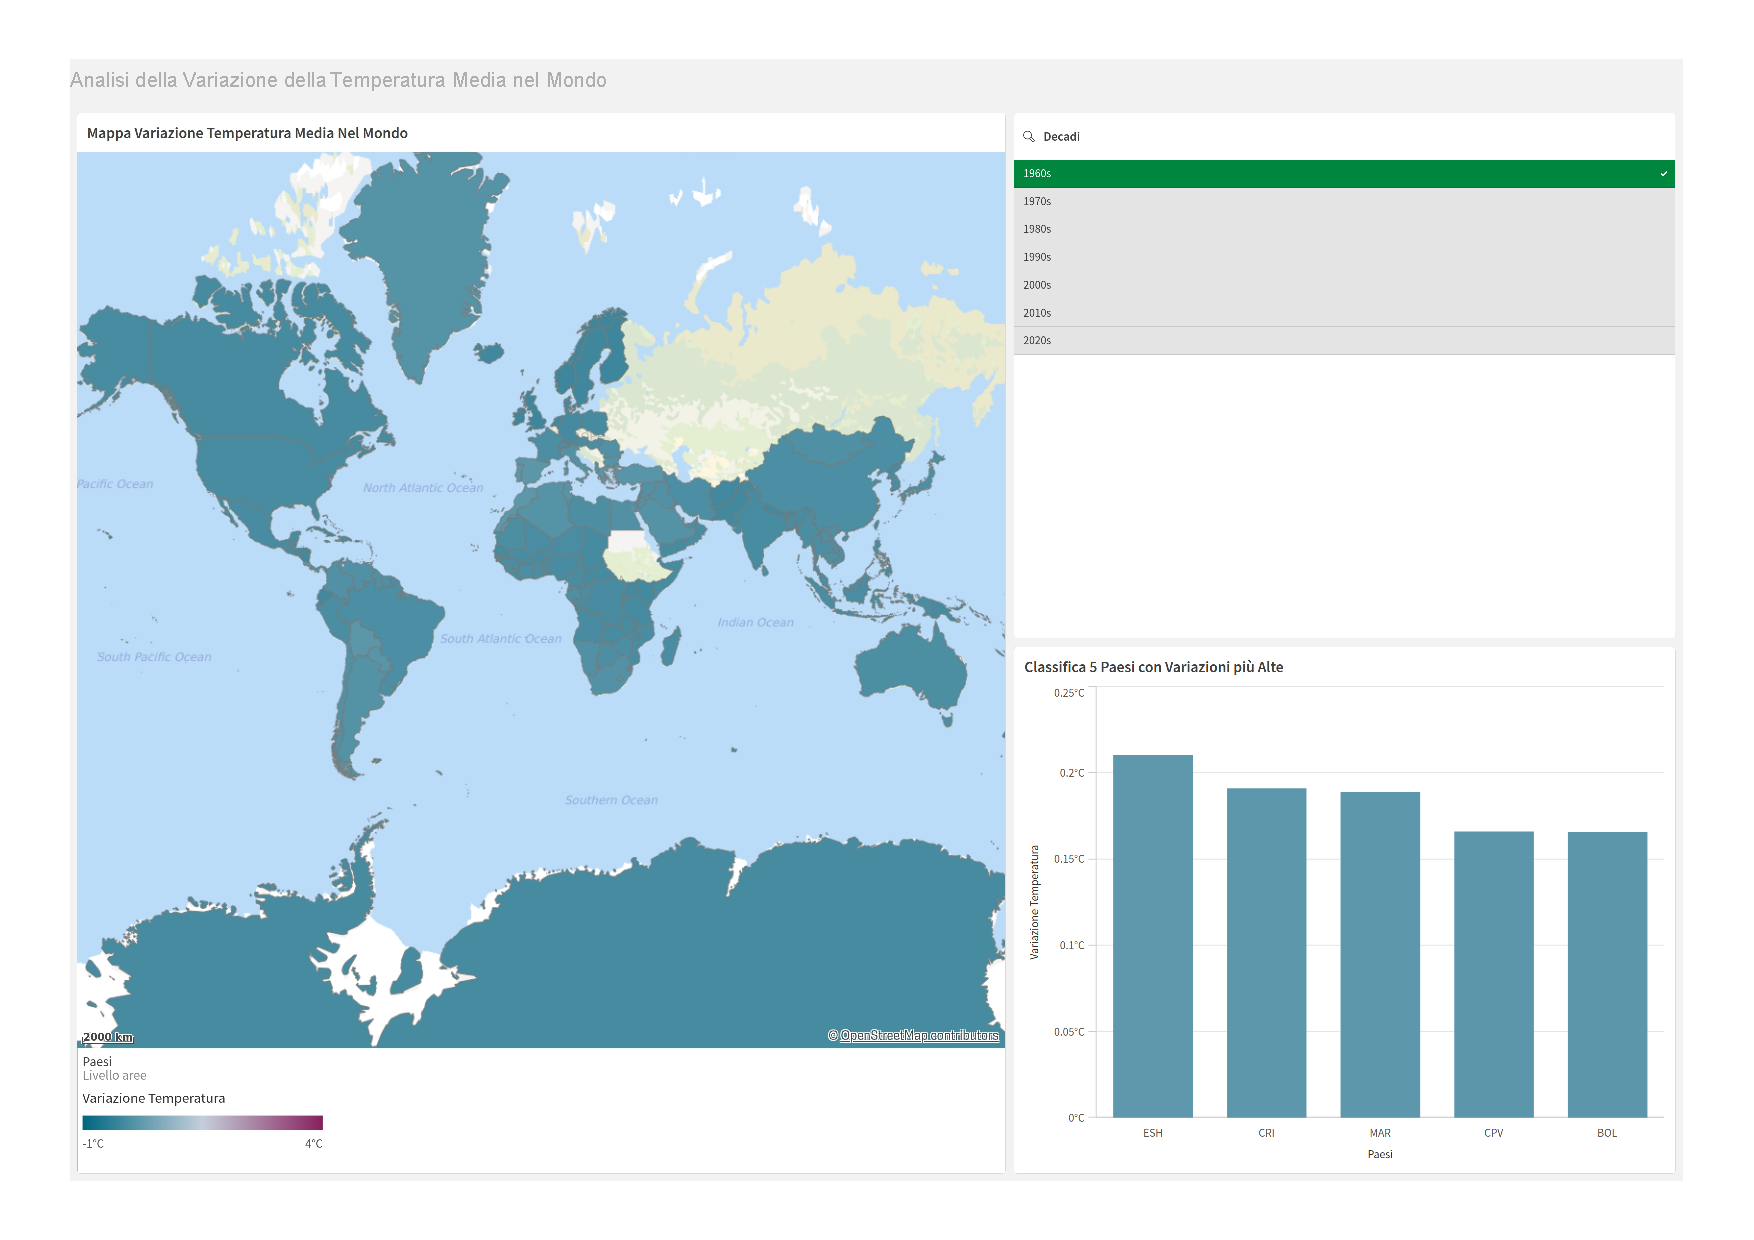
\includegraphics[width=0.98\linewidth]{capitolo_2/img2/2.1 Variazione temperatura media Mondo (1960).pdf}
    \caption{Analisi della variazione della Temperatura Media nel Mondo (1960)}
    \label{fig:2.1}
    \vspace{1mm}
    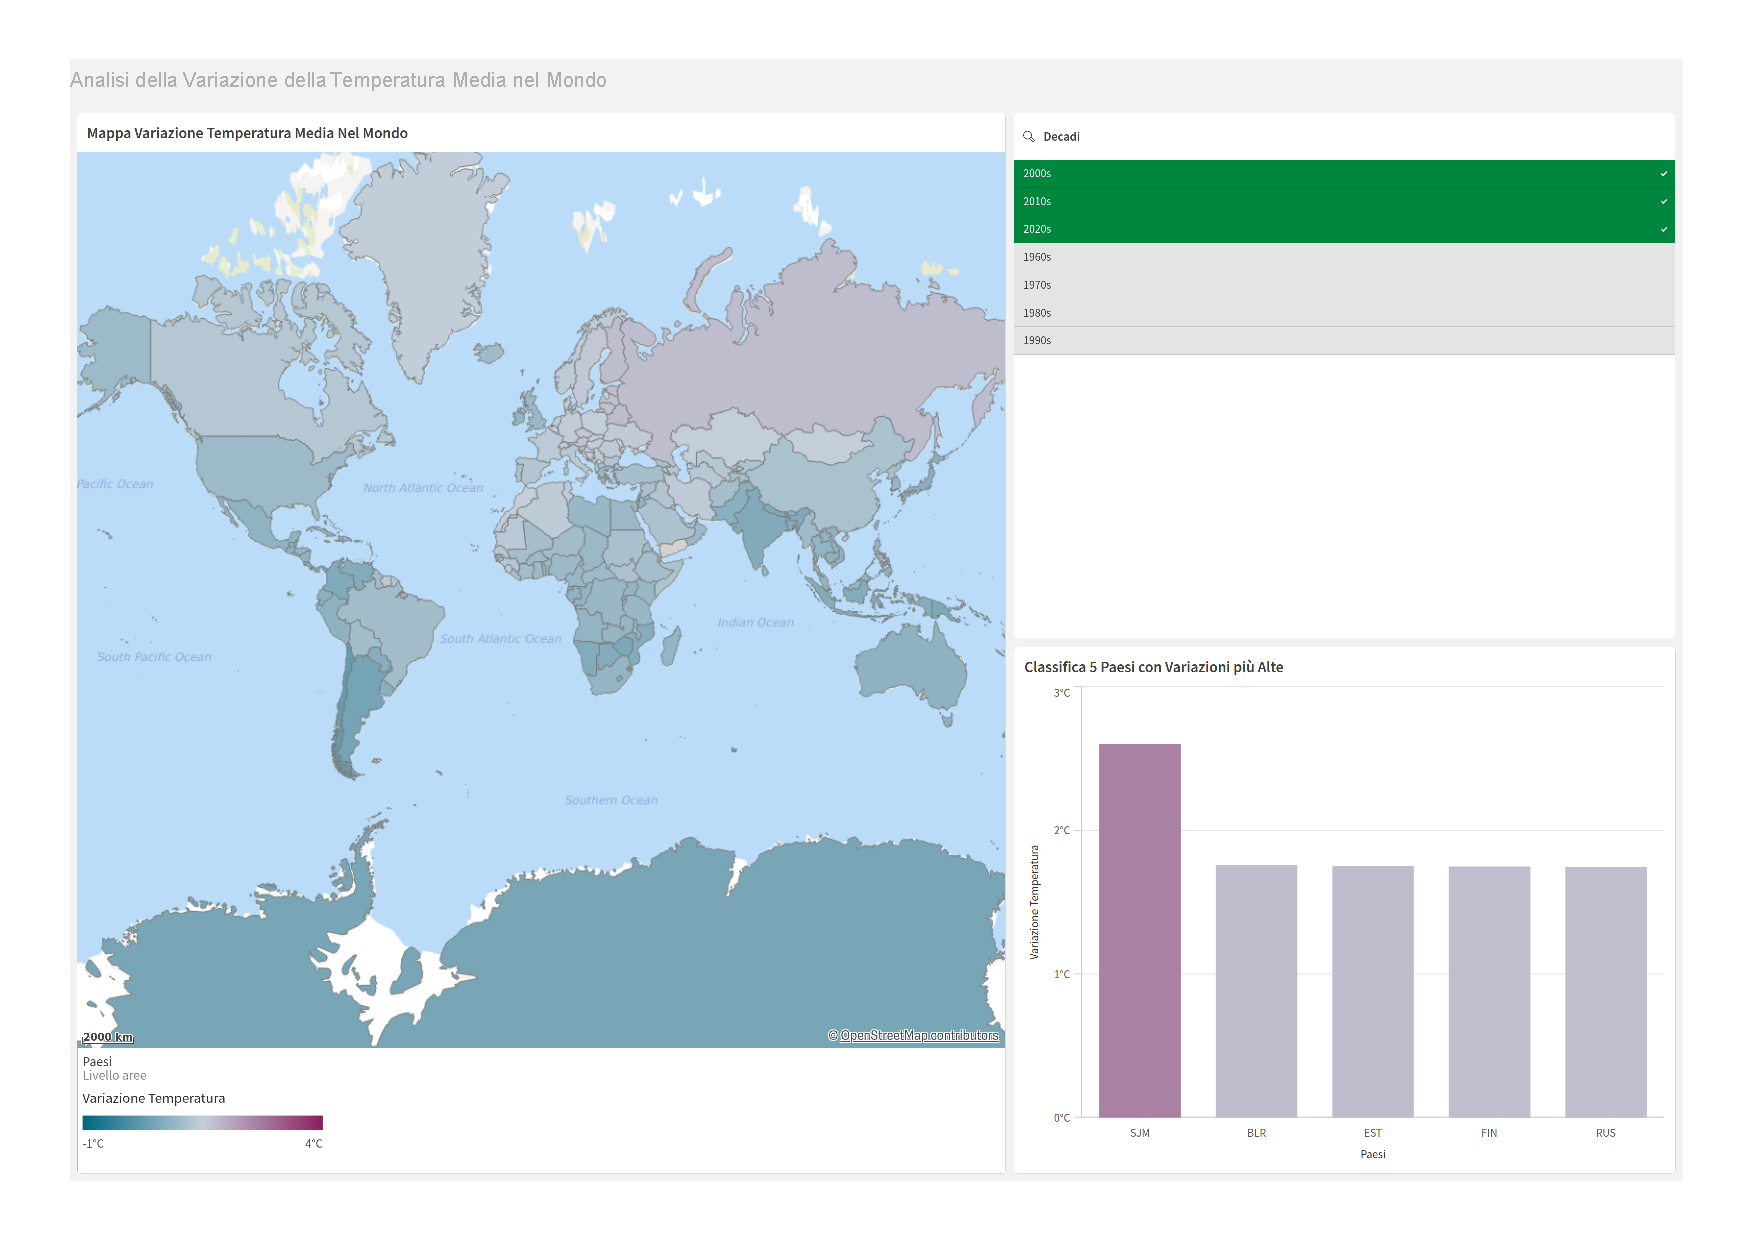
\includegraphics[width=0.98\linewidth]{capitolo_2/img2/2.2 Variazione temperatura media Mondo (00-10-19).pdf}
    \caption{Analisi della variazione della Temperatura Media nel Mondo (2000s-2010s-2020s)}
    \label{fig:2.2}
\end{figure}

Un altro strumento utile fornito dalla Dashboard è il grafico \textbf{Classifica dei 5 Paesi con le Variazioni più Alte}, che consente di individuare i paesi che hanno registrato i cambiamenti di temperatura più significativi, in aumento o in diminuzione, rispetto alla media globale.
Ad esempio, è possibile notare come nella decade \texttt{1960s} lo stato con la variazione più importante sia stato lo Eswatini (ESH), una nazione situata nell'Africa meridionale, con un trend che supera leggermente i \texttt{0.2°C}. Invece, nelle decadi \texttt{2000s-2010s-2020s}, il territorio primo in classifica è quello del Svalbard e Jan Mayen (SJM\footnote{Le Svalbard sono un arcipelago situato nell'Oceano Artico, mentre Jan Mayen è un'isola vulcanica nell'Oceano Artico, anch'essa sotto la sovranità norvegese.}). Da notare come alcuni paesi del Nord Europa abbiano subito un riscaldamento molto rapido, mentre regioni tropicali possano aver mostrato tendenze meno accentuate. Questa analisi aiuta a comprendere come differenti aree del mondo stiano rispondendo al cambiamento climatico, mettendo in evidenza le specificità regionali.
\begin{myoutline}
    \textbf{Nota}: Va precisato che dal 1961 al 1991 gli stati balcanici sono ancora sotto il nome di URSS. Infatti, solo dal 1991 il Soviet Supremo dichiarò l'indipendenza delle 15 repubbliche sovietiche e la dissoluzione formale dell'Unione.
\end{myoutline}

Le analisi fornite dalla Dashboard sono fondamentali per monitorare le tendenze climatiche e prevedere gli impatti su ecosistemi, agricoltura e salute. Ad esempio, l'identificazione di aumenti significativi della temperatura in regioni agricole consente di adottare misure preventive per proteggere i raccolti. Inoltre, la Dashboard è uno strumento utile per sensibilizzare il pubblico e i decisori politici, rendendo visibili le aree più colpite dal riscaldamento globale e promuovendo politiche ambientali sostenibili.

\subsection{Confronto Globale sulle Variazioni della Temperatura Media}
La Dashboard, come mostrato in Figura \ref{fig:3.0}, presenta una struttura visivamente simile a quella della versione precedente, ma con l'aggiunta di funzionalità che permettono un'analisi più dettagliata e mirata. La principale differenza risiede nella capacità di consentire una visualizzazione e un approfondimento delle variazioni di temperatura media attraverso un filtro che permette di selezionare specifici anni e stati. Questa caratteristica consente agli utenti di esaminare in modo più preciso e contestualizzato i cambiamenti climatici, offrendo una panoramica dettagliata delle fluttuazioni termiche su base annuale e geografica. Come per le precenti, per la sua reaizzazione è stato impiegato il dataset \textbf{FAOSTAT Temperature Change}.

\begin{figure}[h!]
    \centering
    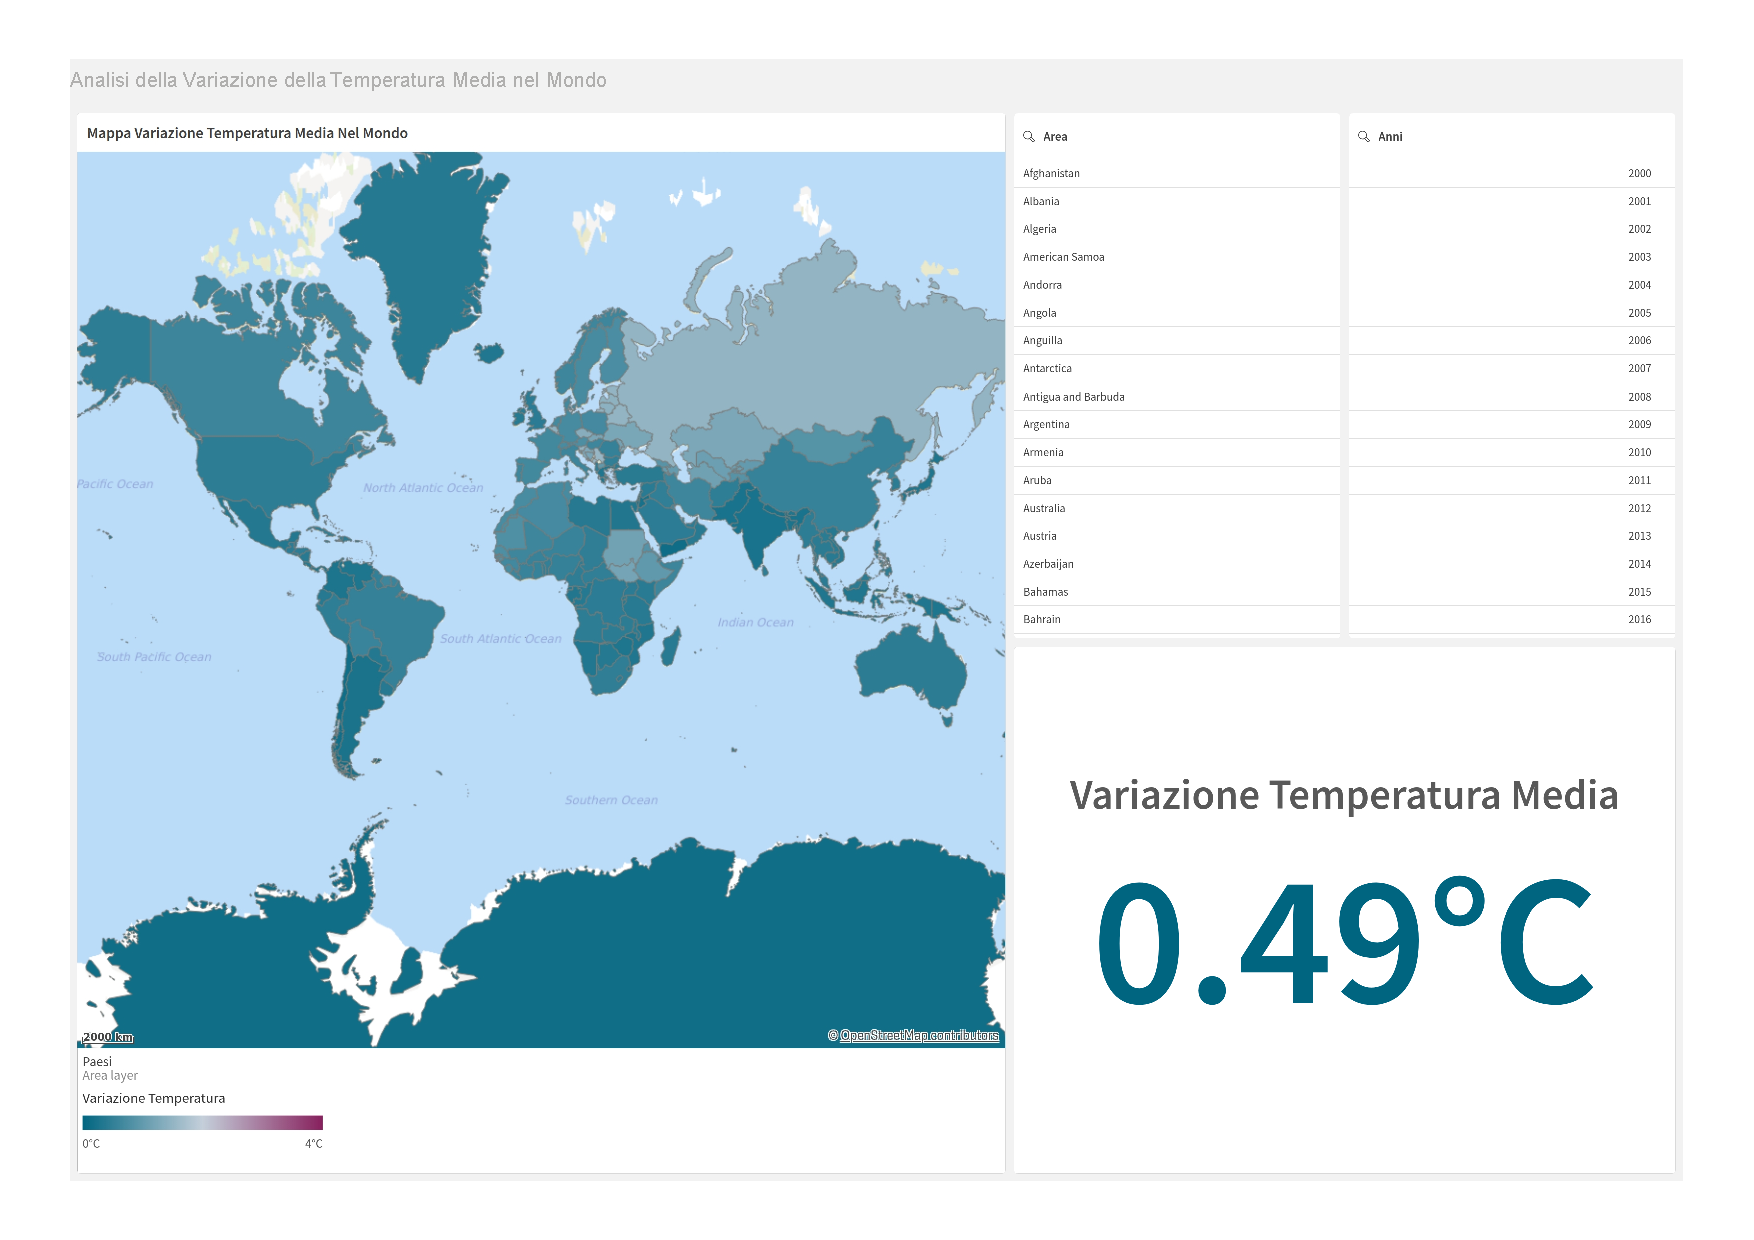
\includegraphics[width=0.98\linewidth]{capitolo_2/img2/3.0 Mappamondo2.pdf}
    \caption{Confronto Globale sulle Variazioni della Temperatura Media}
    \label{fig:3.0}
\end{figure}
\subsubsection{Struttura Dashboard}
La struttura della Dashboard è organizzata in modo da facilitare un'analisi dettagliata delle variazioni termiche. A sinistra, è visibile una visualizzazione geografica denominata \textbf{Mappa della Variazione della Temperatura Media nel Mondo}, dove gli Stati inclusi nell'analisi sono colorati in base alla variazione termica registrata. Questa mappa permette di osservare in modo chiaro le differenze nelle fluttuazioni delle temperature tra le diverse regioni del mondo. A destra, invece, sono presenti due filtri: uno consente la selezione dei singoli Stati, mentre l'altro permette di scegliere gli anni di interesse, compresi tra il 2000 e il 2020. 

\begin{myoutline}
    \textbf{Nota}: La scelta di limitare l'analisi agli anni dal 2000 al 2020 è motivata dalle considerazioni già esposte. Questi anni, infatti, mostrano una variazione termica significativamente maggiore rispetto ai periodi precedenti. Inoltre, l'analisi di questa finestra temporale risulta essere propedeutica per una successiva integrazione con il secondo dataset.
\end{myoutline}

Inoltre, è presente un KPI denominato \textbf{Variazione Temperatura Media}, che fornisce un'indicazione chiara della variazione di temperatura media per lo stato selezionato nel periodo di tempo definito. 

\subsubsection{Obiettivo dell'Analisi}
Questa Dashboard è progettata per fornire uno strumento interattivo e dettagliato per l'analisi delle variazioni della temperatura media globale nel periodo compreso tra il 2000 e il 2020. L'obiettivo principale della Dashboard è quello di permettere agli utenti di esplorare e analizzare l'andamento delle temperature in modo approfondito, consentendo di selezionare specifici Stati e anni per osservare in dettaglio le fluttuazioni termiche.
Ad esempio, come si può notare in Figura \ref{2000}, sono mostrati alcuni risultati ottenuti filtrando le Dashboard in base all'anno, in questo caso il 2000, e agli Stati. In particolare la scelta è ricaduta sull'Italia, la Cina, gli USA e l'India. 

\begin{myoutline}
    \textbf{Nota}: La scelta di analizzare la situazione di Italia, USA, Cina e India è motivata dalla loro rilevanza sia a livello geografico che economico e demografico. Inoltre, l'Italia è stata soggetto di analisi anche della Dashboard in Figura \ref{fig:dashboard_italia}.
\end{myoutline}

\begin{figure}[h!]
  \centering
  \begin{tabular}{cc}  % Crea due colonne
    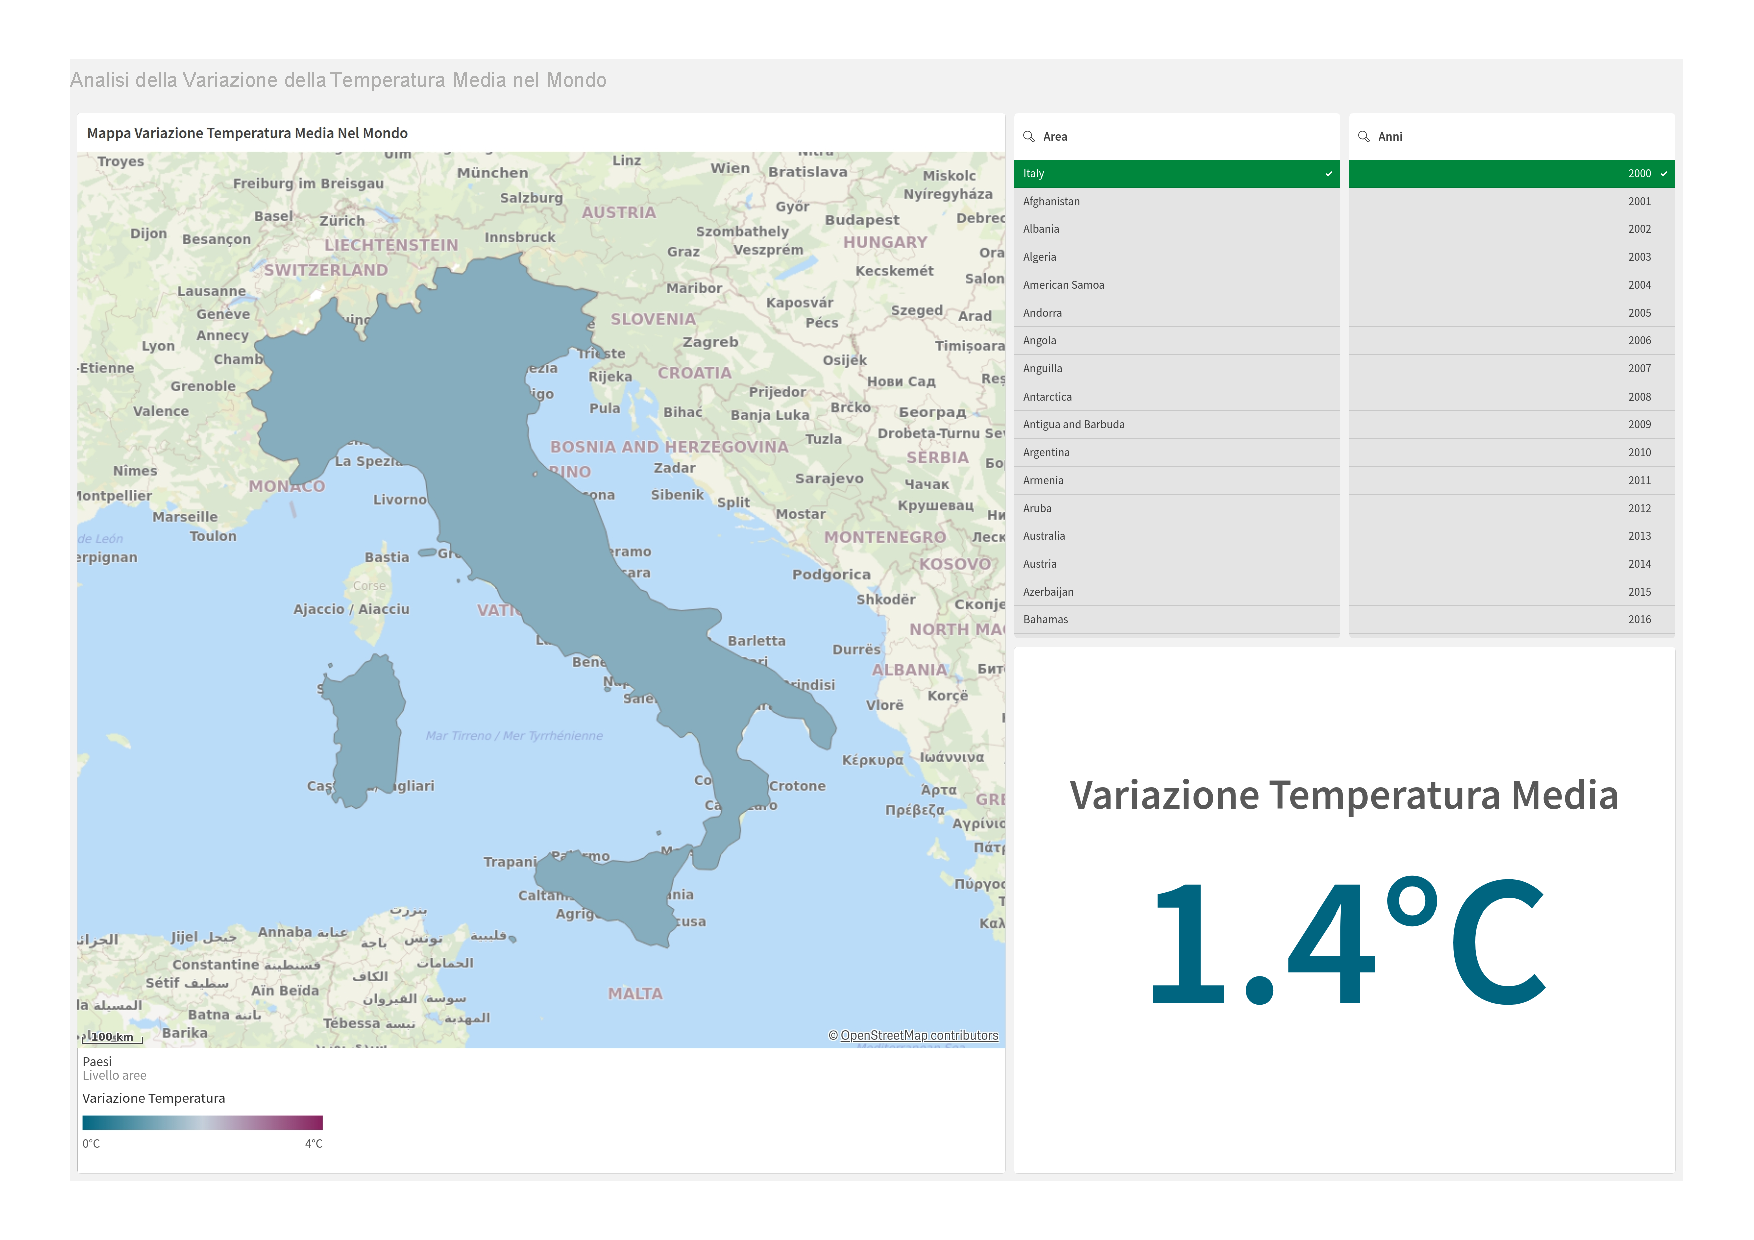
\includegraphics[width=0.45\textwidth]{capitolo_2/img2/3.1 Italia (2000).pdf} & 
    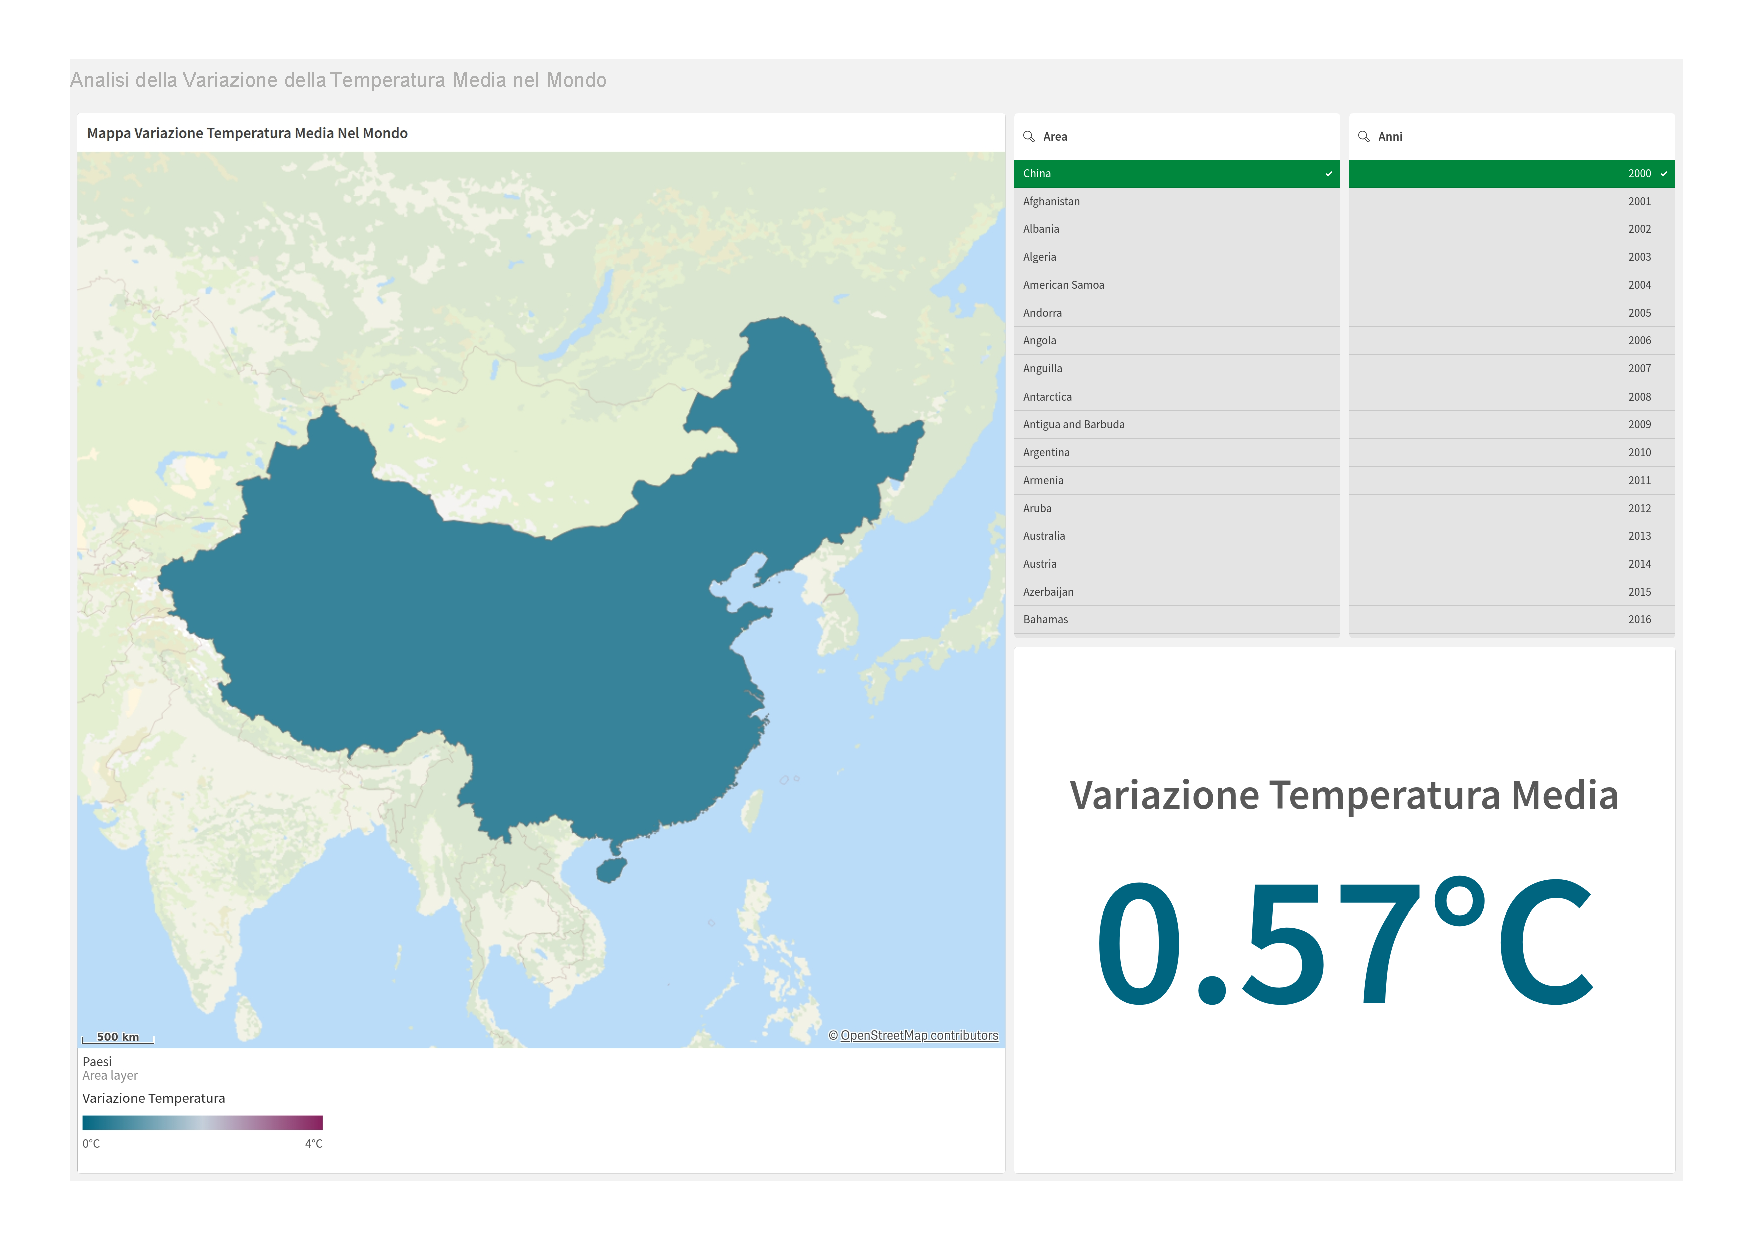
\includegraphics[width=0.45\textwidth]{capitolo_2/img2/3.3 Cina (2000).pdf} \\  % Prima riga
    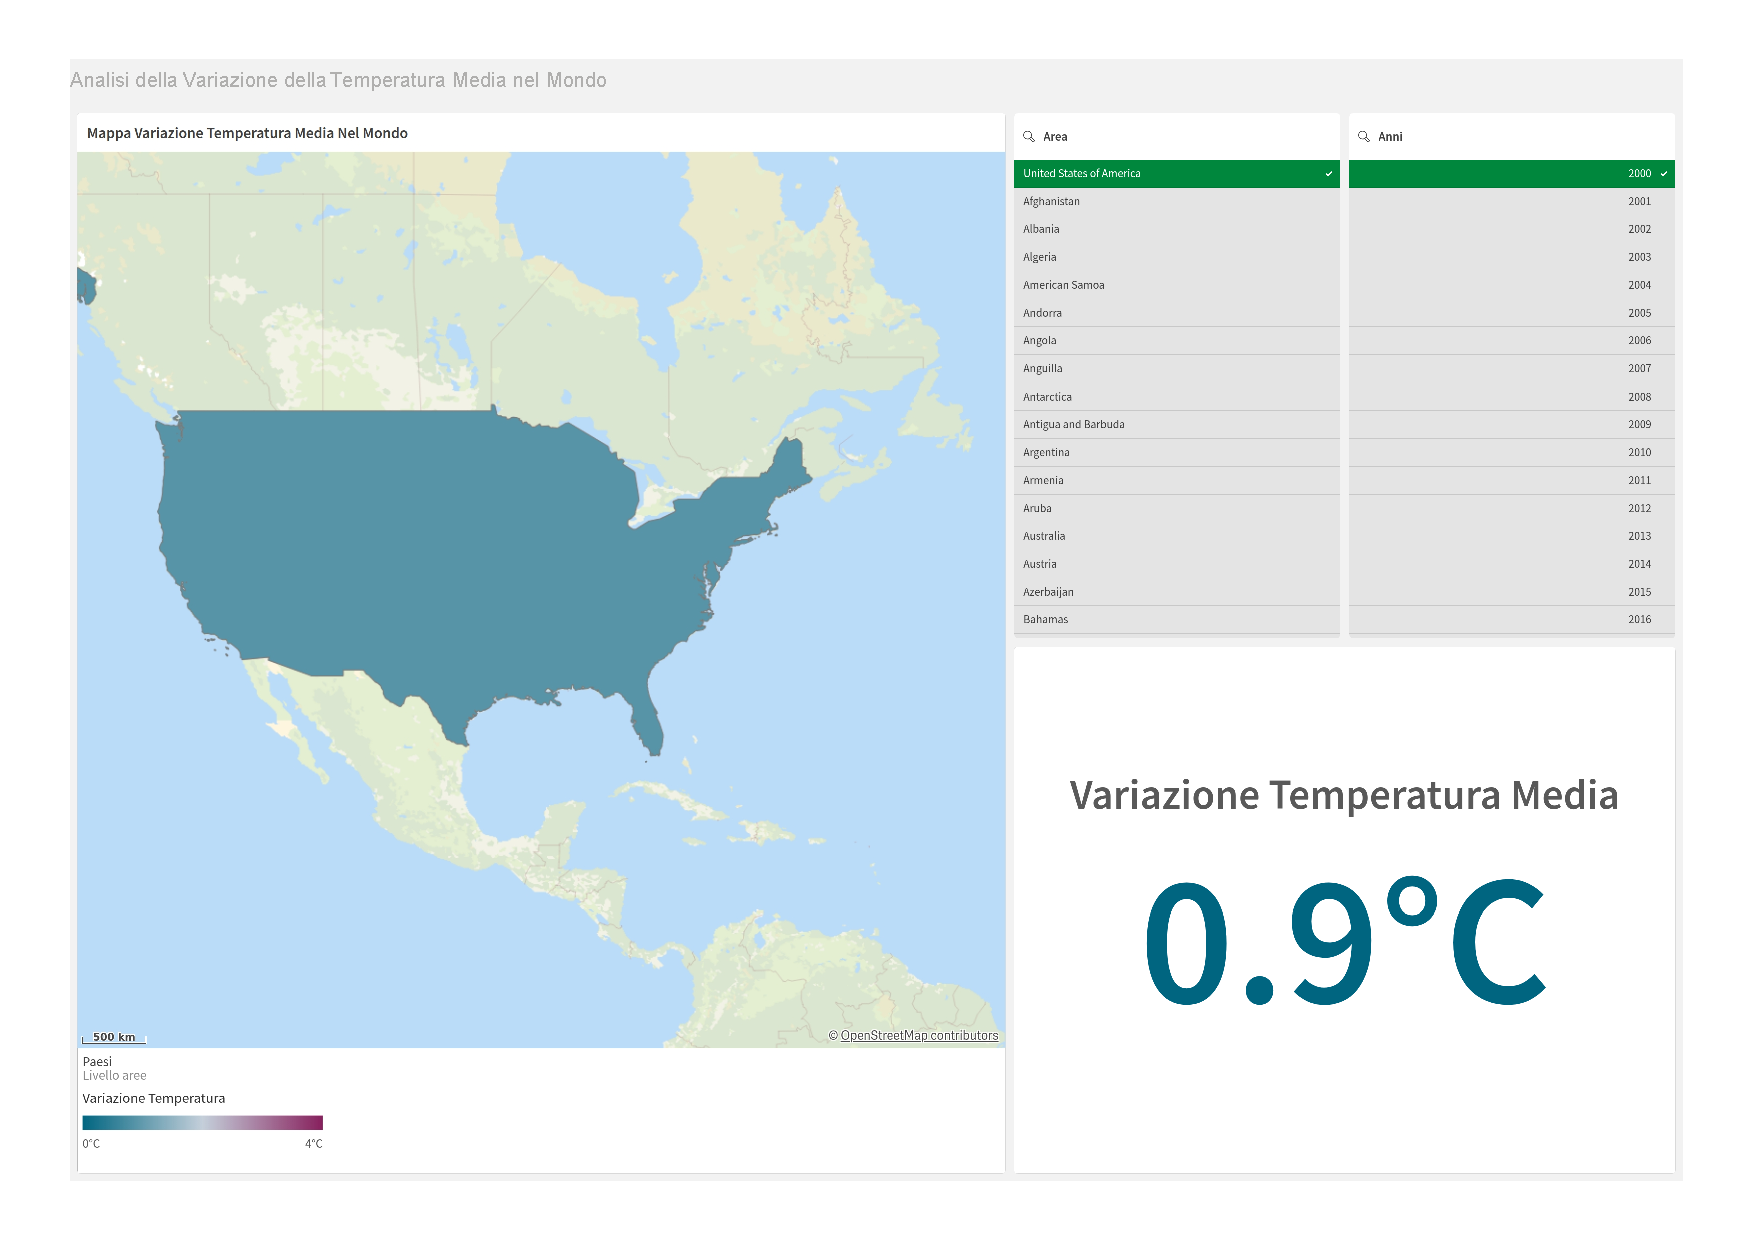
\includegraphics[width=0.45\textwidth]{capitolo_2/img2/3.5 USA (2000).pdf} & 
    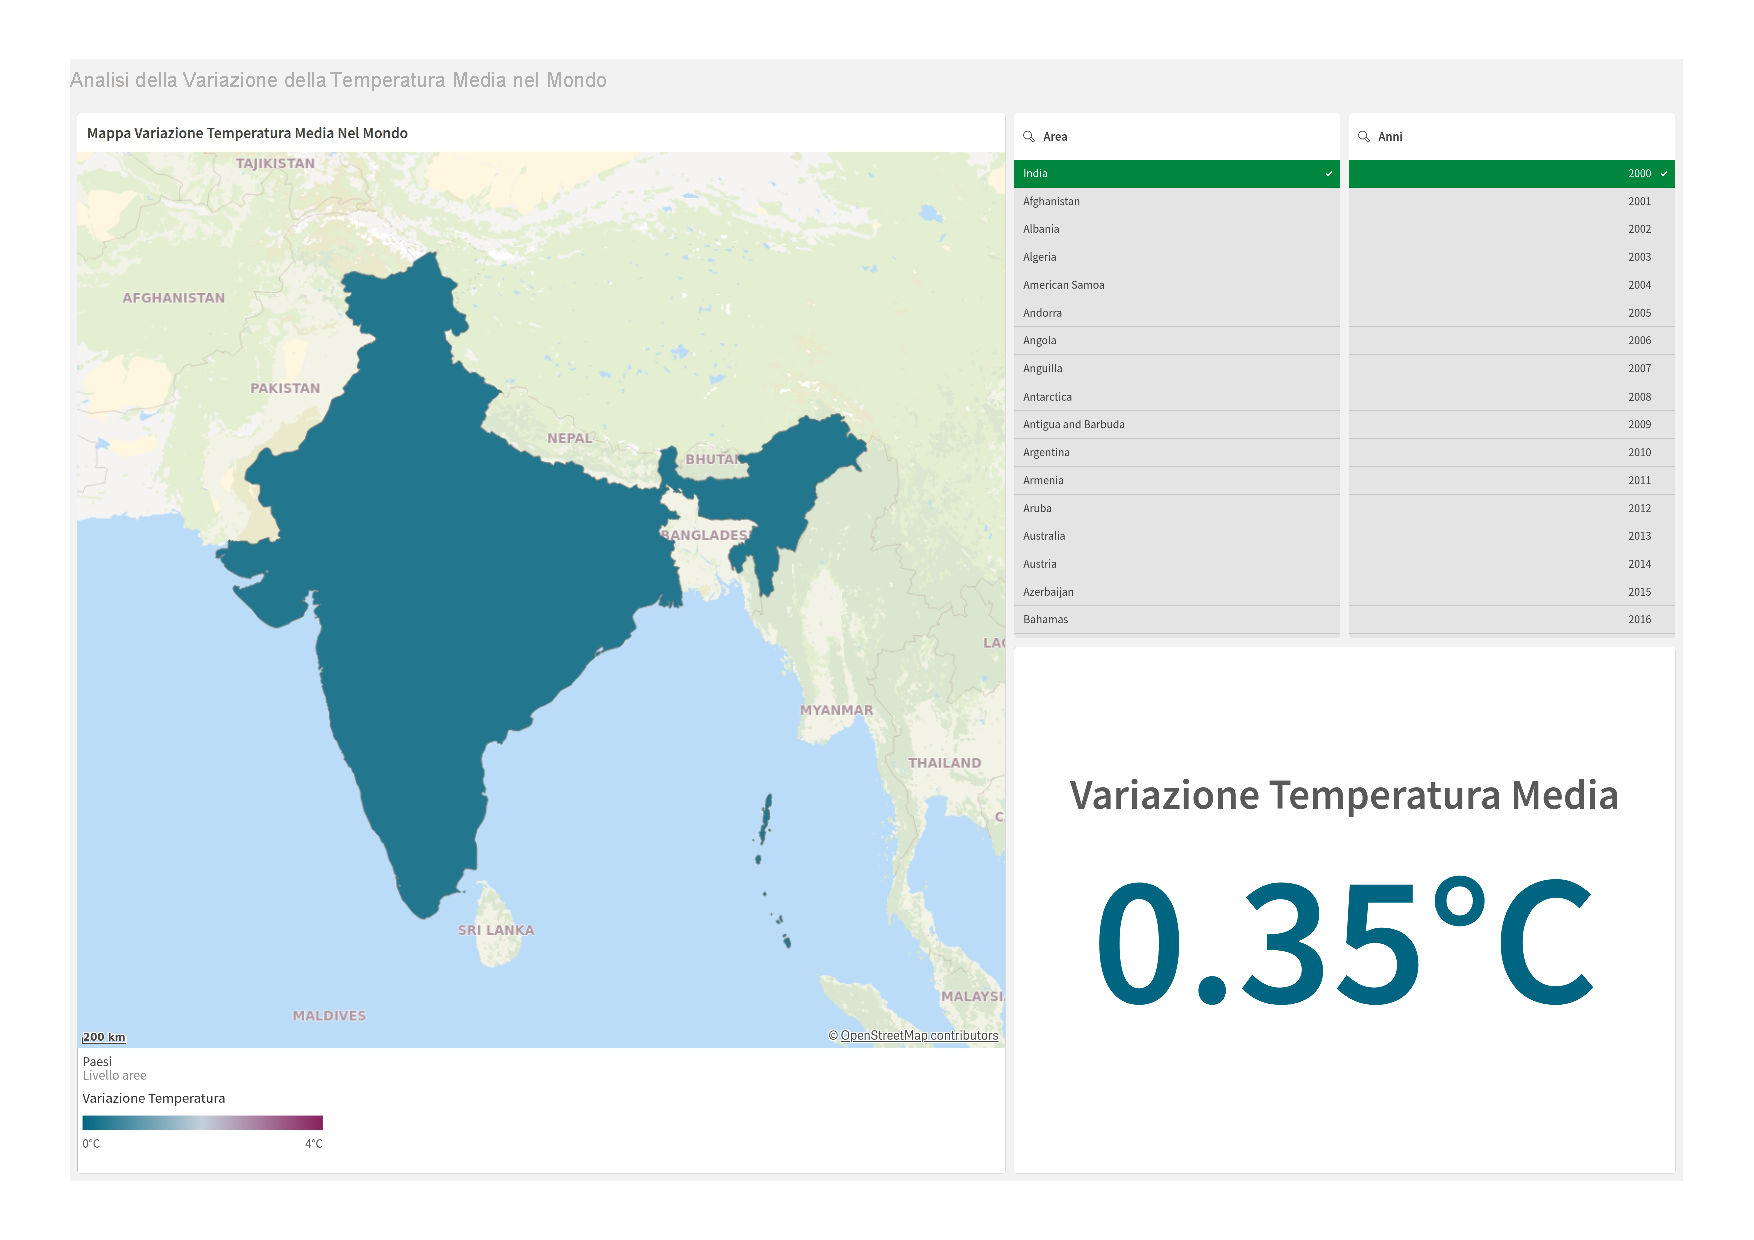
\includegraphics[width=0.45\textwidth]{capitolo_2/img2/3.7 India (2000).pdf} \\  % Seconda riga
  \end{tabular}
  \caption{Confronto sulle Variazioni della Temperatura Media in Italia, Cina, USA e India nel 2000}
  \label{2000}
\end{figure}

Come si può osservare, l'Italia, pur avendo una superficie geografica e una popolazione nettamente inferiori rispetto ad altri Stati, mostra una variazione di temperatura media significativamente più elevata, pari a \texttt{1.4°C}. Al contrario, stati come la Cina, pur avendo dimensioni geografiche e demografiche molto più ampie, registrano una variazione termica inferiore. Riprendendo le analisi presentate in Figura \ref{fig:dashboard_italia}, è evidente come l'Italia abbia subito un incremento della temperatura molto più pronunciato rispetto alla media globale, suggerendo che il paese stia affrontando sfide climatiche particolarmente rilevanti in relazione ad altre regioni del mondo. Invece, altri paesi come l'India, presentano una variazione addirittura al di sotto della media calcolata, pari al \texttt{0.49°C}.

In Figura \ref{2019}, sono illustrate le analisi relative al 2019, basate sugli stessi Stati presi in considerazione in precedenza. Come si può osservare, ogni Stato ha registrato un incremento significativo della variazione della temperatura in un periodo di tempo relativamente breve. Questo evidenzia come, anche in lassi di tempo ridotti, i cambiamenti climatici stiano accelerando in modo evidente, con un impatto tangibile su molteplici regioni del mondo.

\begin{figure}[h!]
  \centering
  \begin{tabular}{cc}  % Crea due colonne
    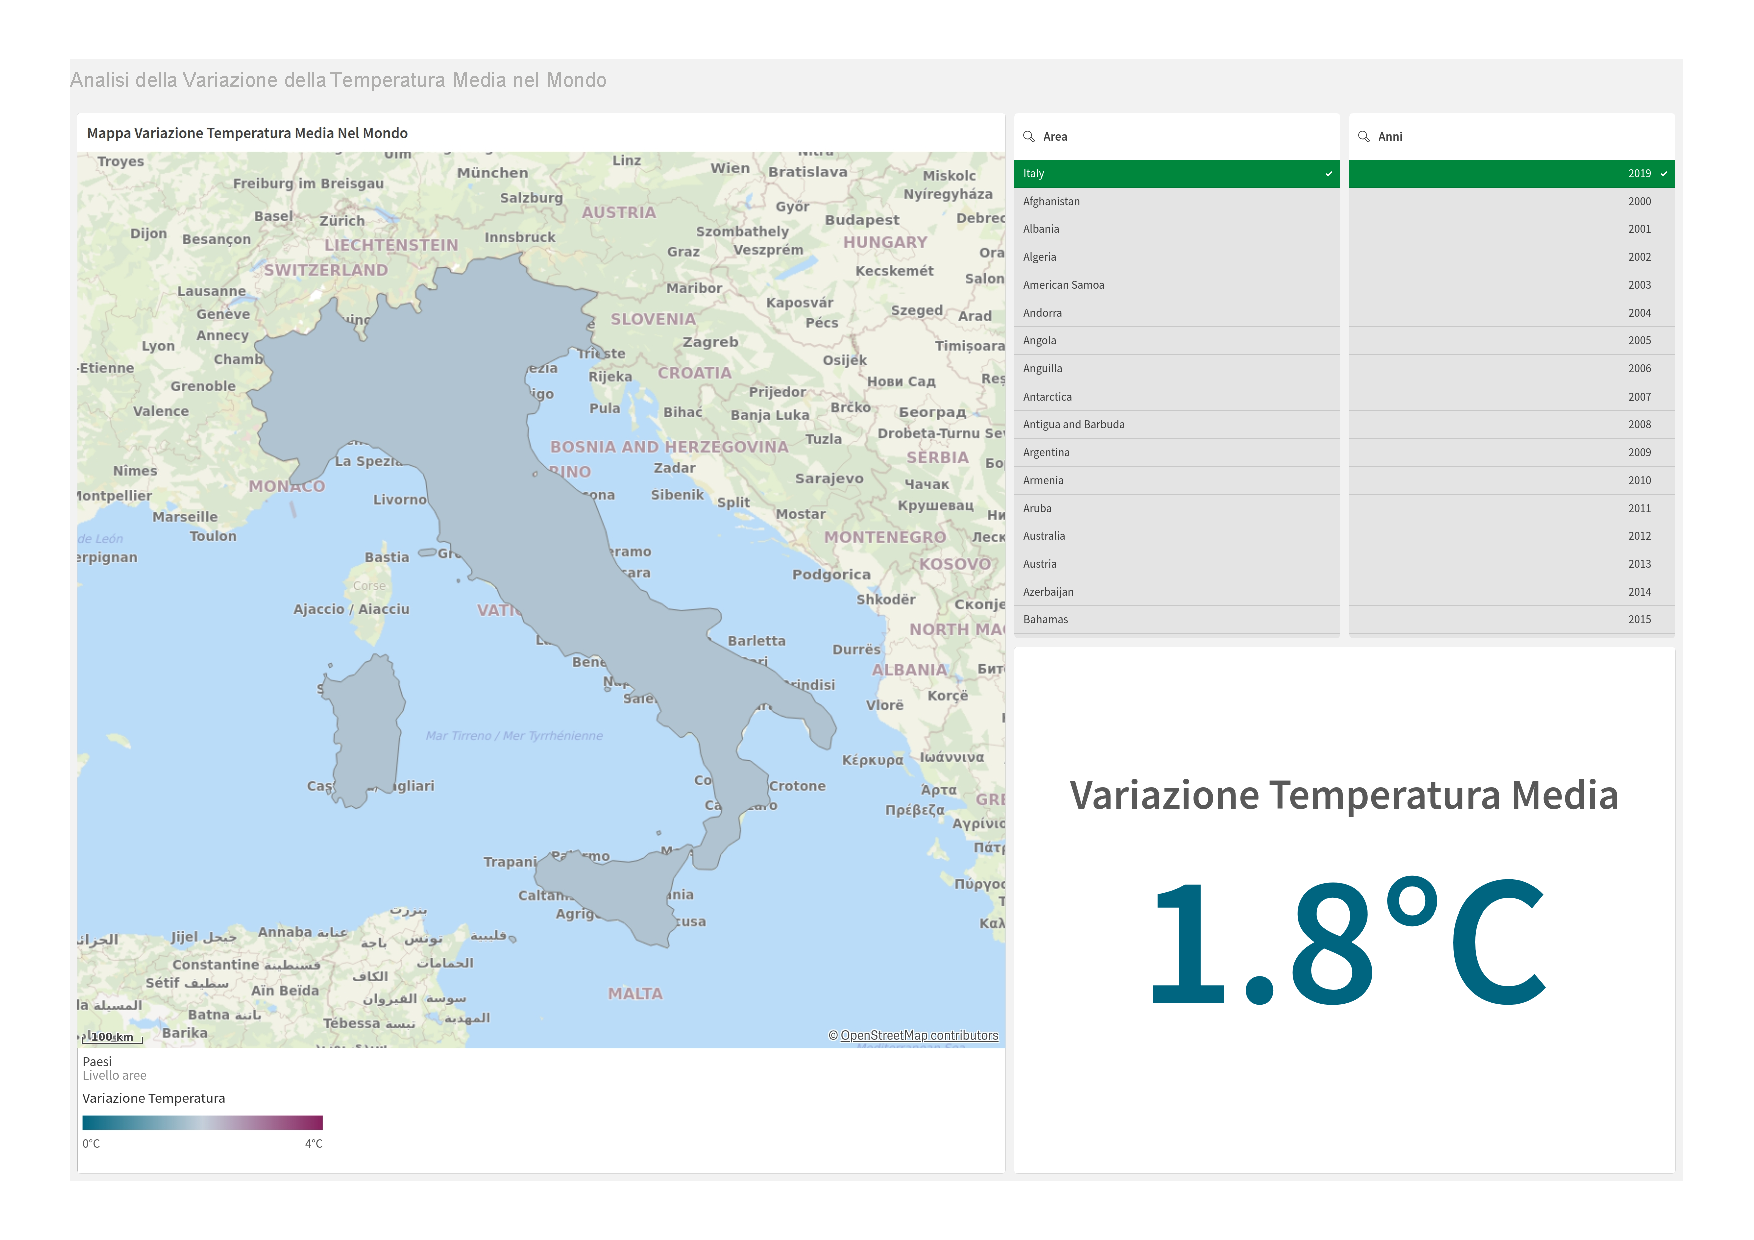
\includegraphics[width=0.45\textwidth]{capitolo_2/img2/3.2 Italia (2019).pdf} & 
    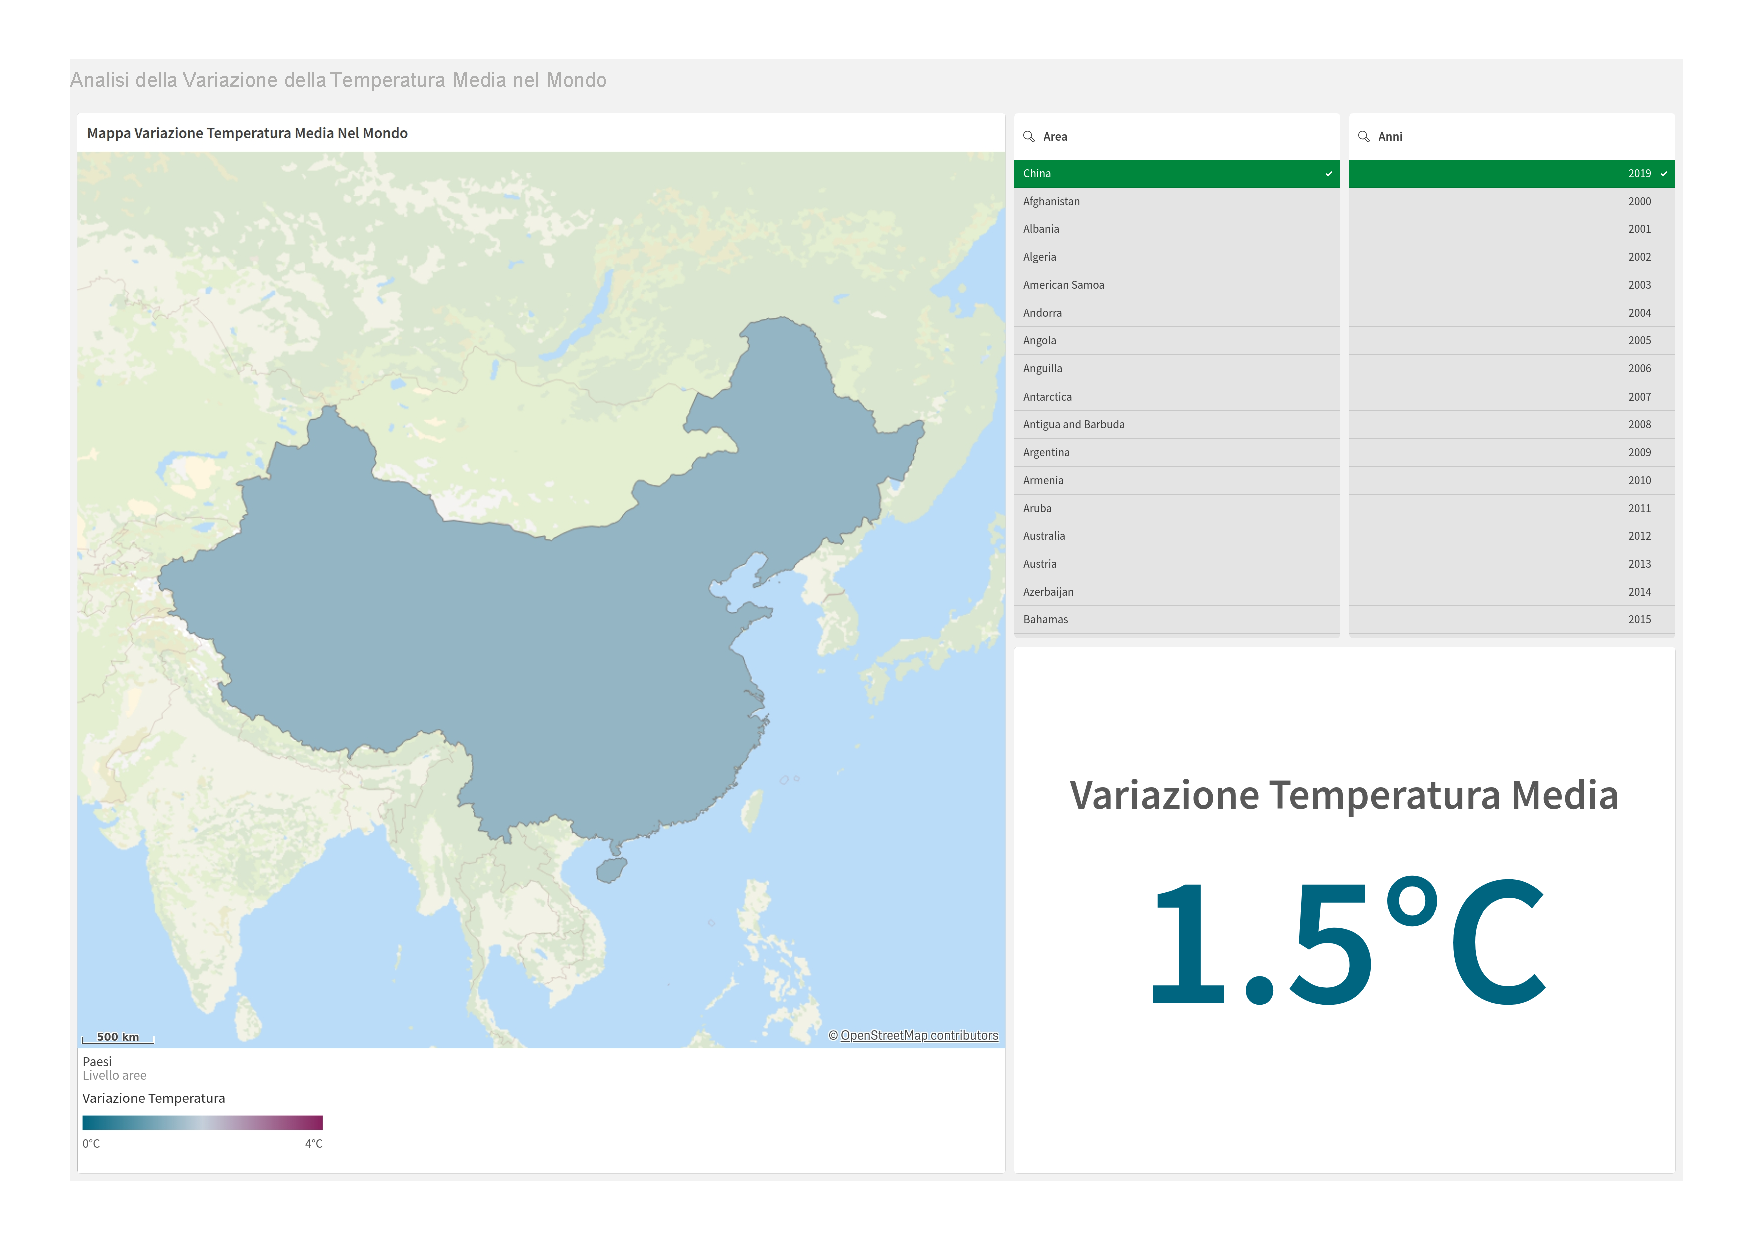
\includegraphics[width=0.45\textwidth]{capitolo_2/img2/3.4 Cina (2019).pdf} \\  % Prima riga
    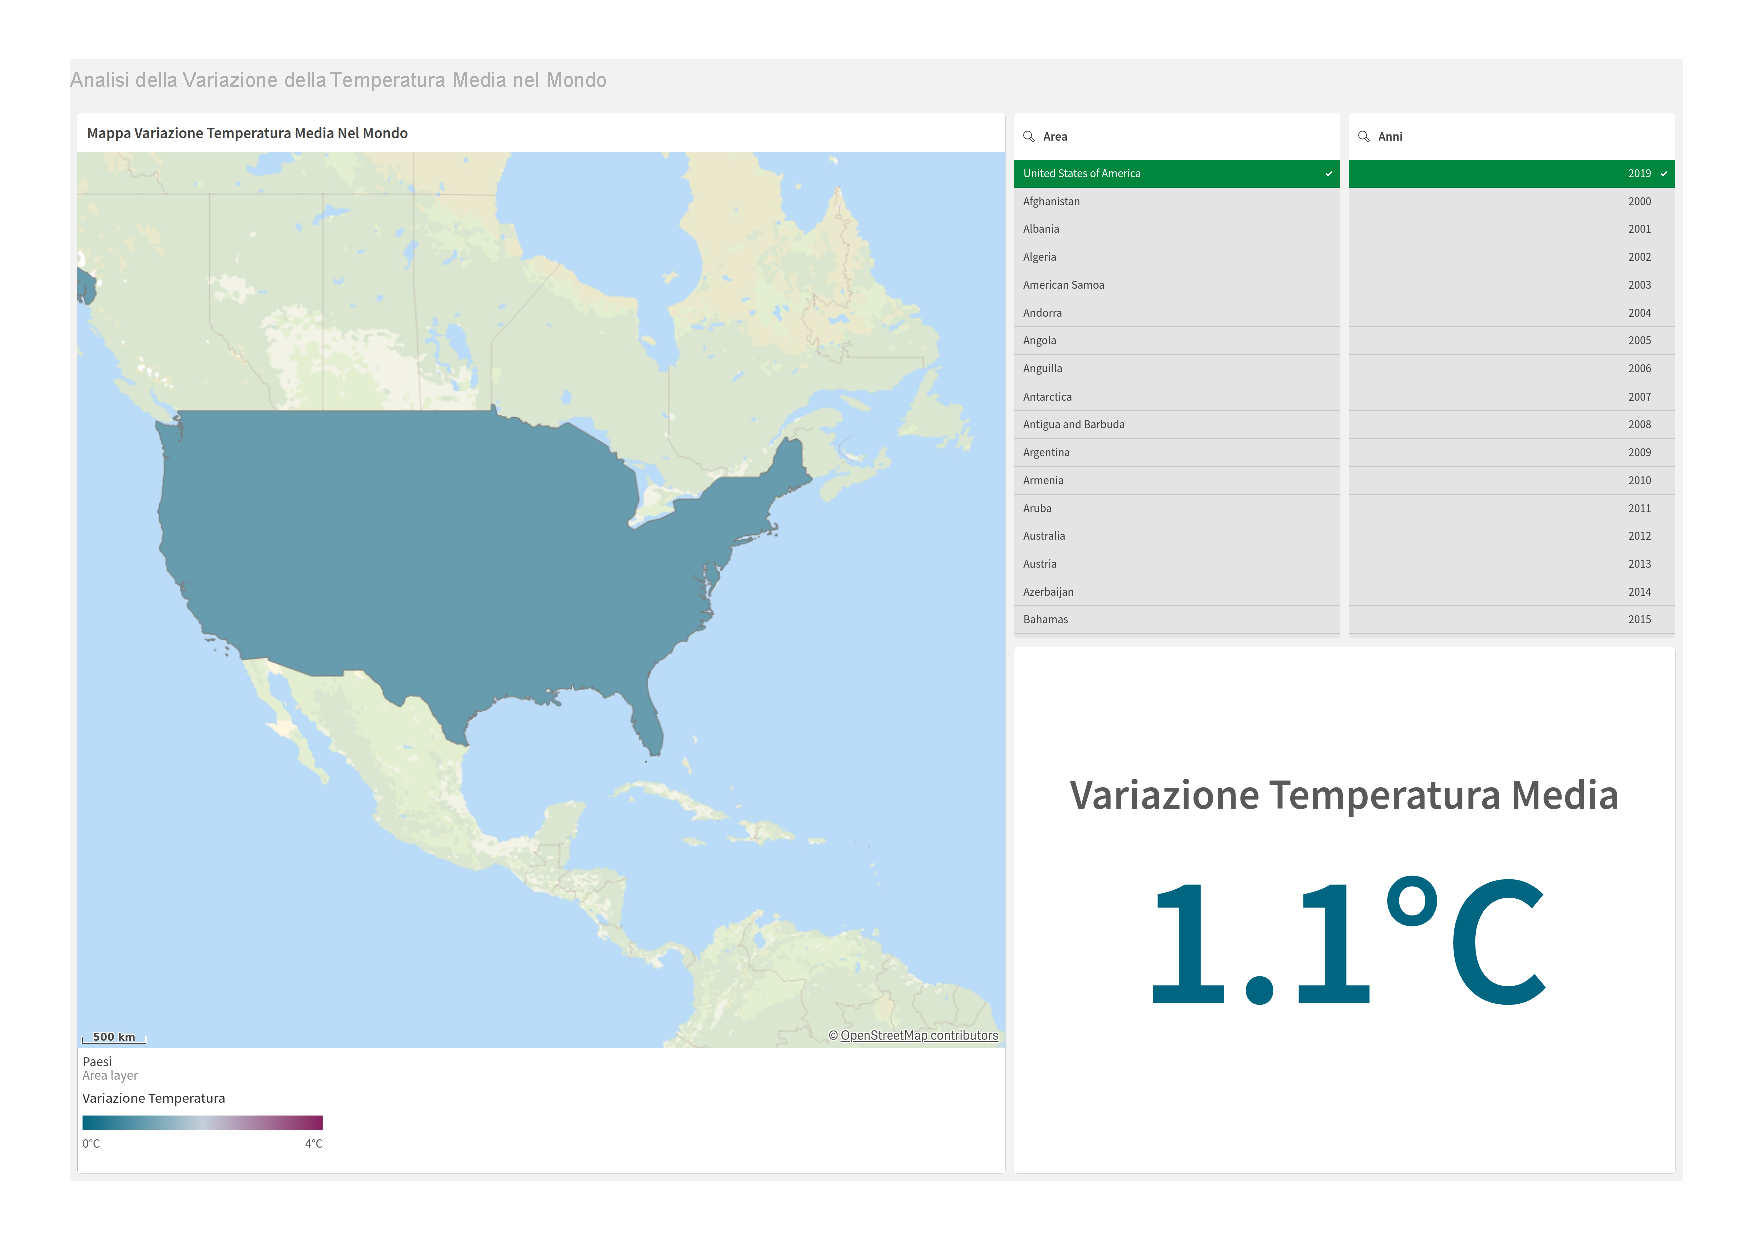
\includegraphics[width=0.45\textwidth]{capitolo_2/img2/3.6 USA (2019).pdf} & 
    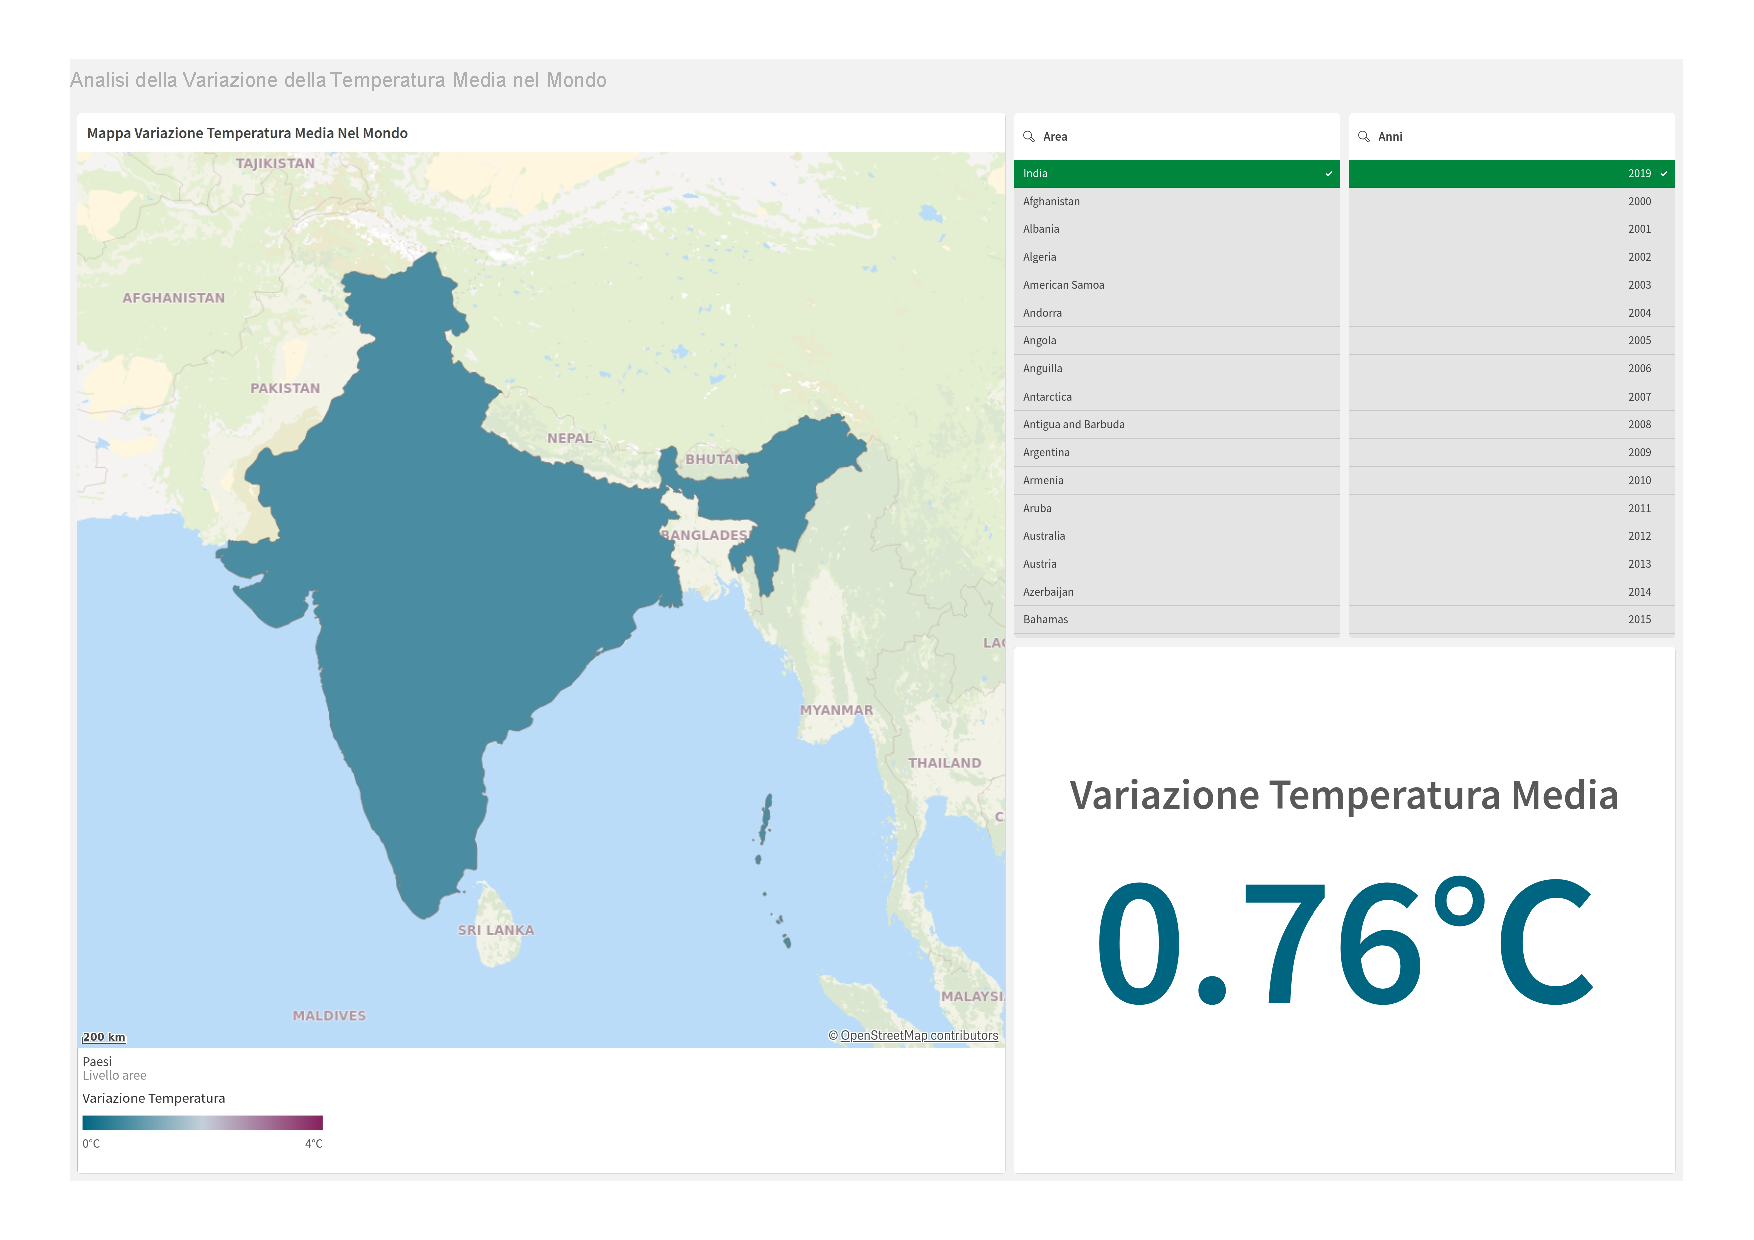
\includegraphics[width=0.45\textwidth]{capitolo_2/img2/3.8 India (2019).pdf} \\  % Seconda riga
  \end{tabular}
  \caption{Analisi della Variazione della Temperatura Media in Italia, Cina, USA e India nel 2019}
  \label{2019}
\end{figure}


%4.0
\subsection{Tendenze Climatiche e CO\textsubscript{2}}
\label{Sezione_4}
La Dashboard, come mostrato in Figura \ref{fig:4.0}, fornisce una rappresentazione chiara e interattiva dell'andamento delle emissioni globali di CO\textsubscript{2} e delle variazioni della temperatura media dal 2000 al 2019. Attraverso un insieme di visualizzazioni grafiche e indicatori chiave, è possibile esplorare i dati e analizzare come i principali Paesi contribuiscano alle emissioni globali e quale correlazione esista tra l'aumento delle emissioni e il cambiamento climatico. Per la costruzione della Dashboard è stato utilizzato il dataset \textbf{FAOSTAT Temperature Change}, integrato al secondo dataset chiamato \textbf{Global Data on Sustainable Energy (2000-2020)}.

L'analisi si concentra principalmente sull'andamento delle emissioni nei singoli anni e sul confronto tra le diverse nazioni, evidenziando le economie più responsabili delle emissioni. Inoltre, la Dashboard permette di osservare l'incremento complessivo della temperatura globale nello stesso periodo, offrendo una visione d'insieme delle tendenze climatiche in relazione alle emissioni di gas serra.

\subsubsection{Struttura Dashboard}
La Dashboard è organizzata in modo da facilitare un'analisi dettagliata delle emissioni di CO\textsubscript{2} e delle variazioni di temperatura. Gli elementi principali sono disposti strategicamente per garantire una consultazione chiara e intuitiva.

In alto a sinistra è presente un grafico a barre (\textbf{Tendenze climatiche e CO\textsubscript{2}}), che mostra i primi 20 Paesi al mondo per emissioni di CO\textsubscript{2}, espresse in kilotoni. Questo grafico consente di identificare immediatamente le nazioni con il maggiore impatto ambientale e di confrontare i livelli di emissione tra di esse.

Nella parte inferiore della Dashboard sono presenti due KPI che forniscono informazioni sintetiche sull'andamento delle emissioni e della temperatura globale. In basso a sinistra, è riportato il \textbf{valore totale delle emissioni di CO\textsubscript{2}}, espresso in kilotoni, che rappresenta l'ammontare complessivo delle emissioni per l'anno selezionato. In basso a destra, invece, è visualizzato il valore totale della \textbf{variazione della temperatura globale}, espresso in gradi Celsius, che mostra l'incremento della temperatura.

Per permettere un'analisi dinamica e personalizzata, in alto a destra è stato integrato un filtro per la selezione dell'anno, che consente agli utenti di visualizzare i dati relativi a un anno specifico compreso tra il 2000 e il 2019. Attraverso questo strumento, è possibile osservare l'evoluzione delle emissioni e della temperatura nel tempo e identificare eventuali tendenze o cambiamenti significativi.

\begin{figure}[h!]
    \centering
    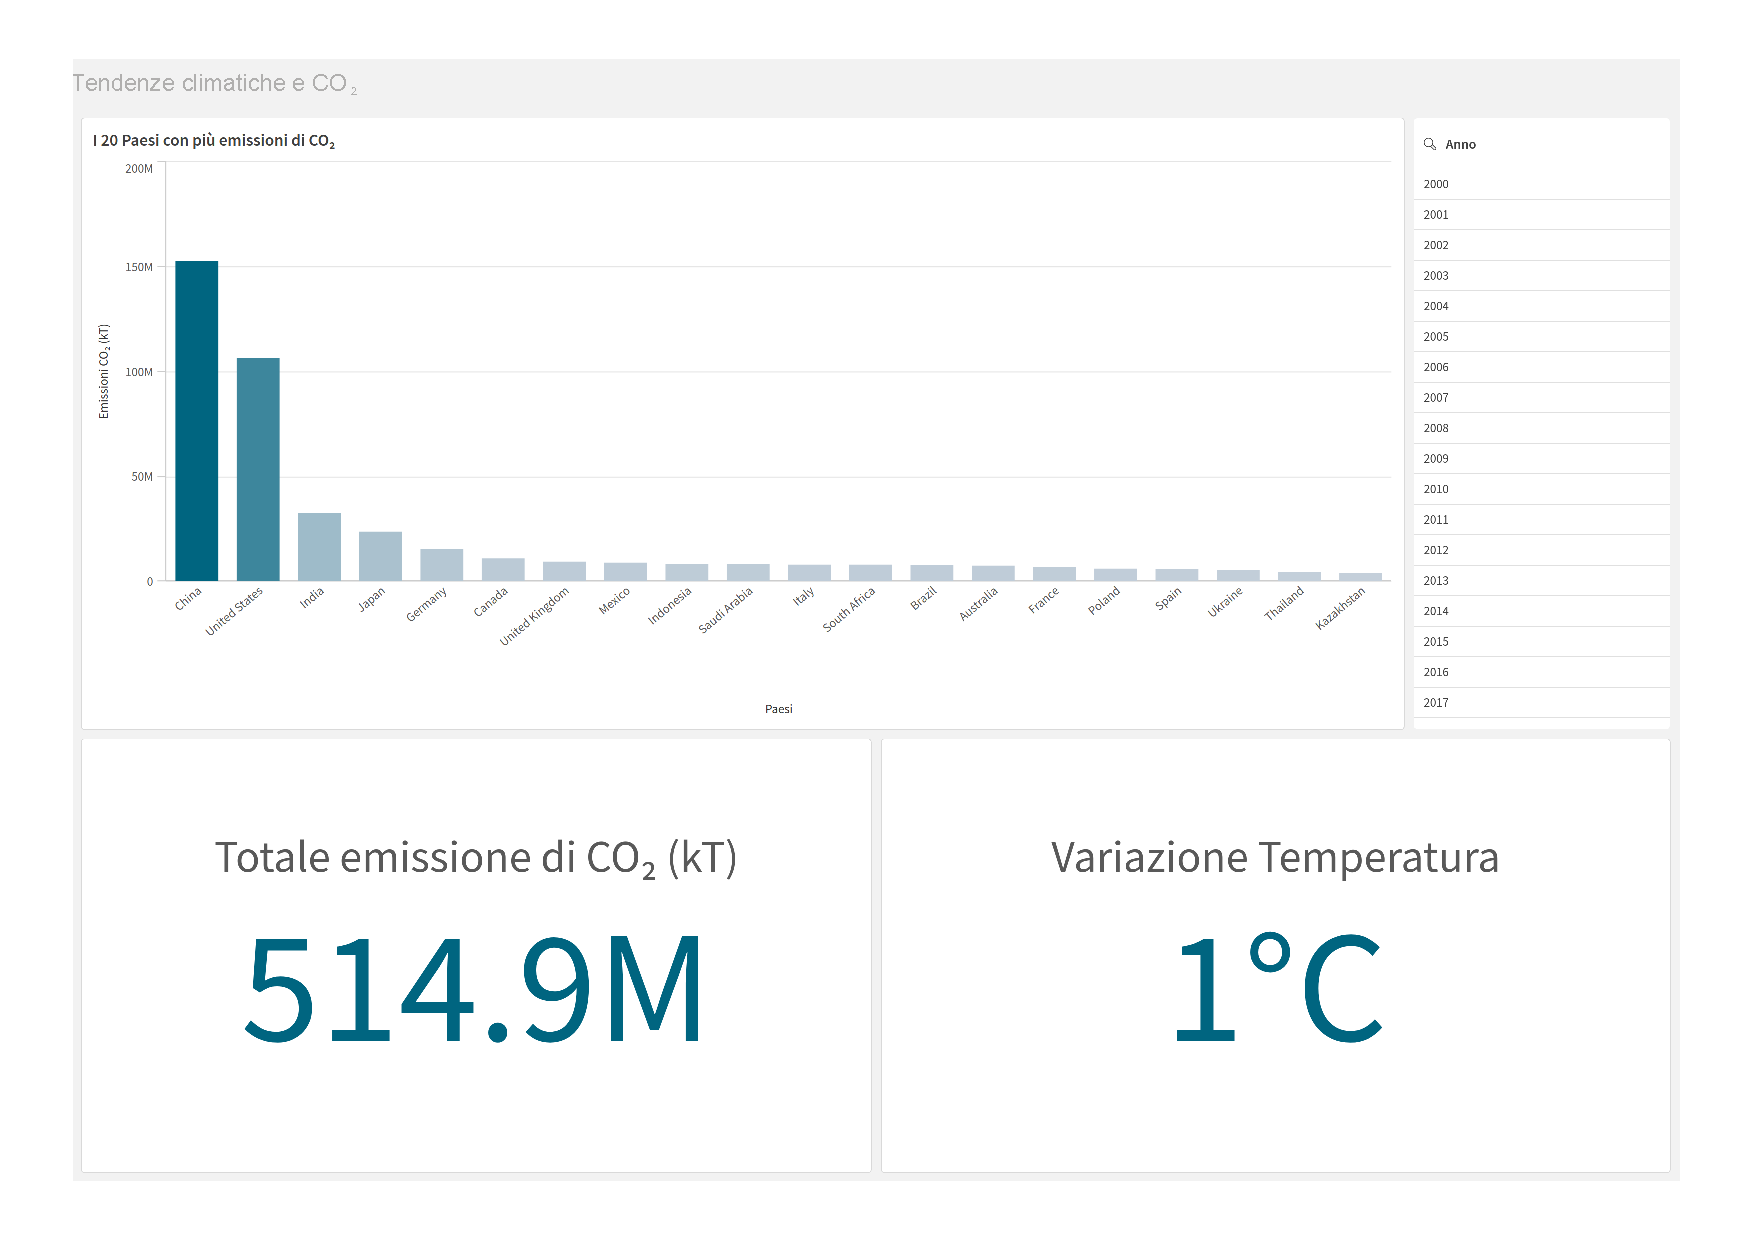
\includegraphics[width=0.98\linewidth]{capitolo_2/img2/4.0 Analisi generale tutti gli anni.pdf}
    \caption{Tendenze Climatiche e CO\textsubscript{2}, panoramica generale}
    \label{fig:4.0}
\end{figure}

\subsubsection{Obiettivo dell'Analisi}
L'obiettivo principale della Dashboard in Figura \ref{CO2} è fornire uno strumento interattivo e dettagliato per comprendere l'evoluzione delle emissioni di gas serra e il loro impatto sulle temperature globali. La possibilità di selezionare specifici anni e Paesi permette di esplorare le correlazioni tra l'incremento delle emissioni e il riscaldamento globale, facilitando l'analisi delle tendenze climatiche e delle strategie adottate dalle diverse nazioni.

\begin{myoutline}
    \textbf{Nota}: La scelta degli anni 2000-2010-2019 è motivata dalla volontà di voler esplorare l'andamento complessivo delle emissioni di CO\textsubscript{2} nell'intero periodo considerato.
\end{myoutline}

L'analisi si focalizza in particolare sull'aumento delle emissioni globali nel periodo considerato. Nel 2000, le emissioni di CO\textsubscript{2} ammontavano a 20 milioni di kilotoni, con una variazione della temperatura pari a 0.68°C. Dopo un decennio, nel 2010, le emissioni hanno raggiunto i 26.84 milioni di kilotoni e la temperatura è salita a 1.1°C, segnalando un'accelerazione del riscaldamento globale. Nel 2019, il valore è salito ulteriormente fino a 29.61 milioni di kilotoni, con una variazione della temperatura che ha toccato 1.5°C, soglia considerata critica dagli scienziati per evitare conseguenze climatiche irreversibili.

Oltre a quantificare le emissioni su scala globale, la Dashboard permette di analizzare la distribuzione delle emissioni tra i diversi Paesi. I dati evidenziano come un numero ristretto di nazioni, principalmente economie avanzate o in forte industrializzazione, sia responsabile della maggior parte delle emissioni globali. Nel 2000, gli Stati Uniti risultavano il principale emettitore mondiale, ma nel corso del decennio successivo la Cina ha rapidamente superato tutti gli altri Paesi, diventando la nazione con le emissioni più elevate. Questa tendenza è strettamente legata alla sua rapida crescita industriale e all'elevato utilizzo di combustibili fossili come fonte di energia.
L'analisi evidenzia inoltre l'effetto delle politiche di riduzione adottate da alcuni Paesi. Se da un lato le economie emergenti, come Cina e India, hanno visto un aumento significativo delle emissioni, dall'altro Paesi come quelli dell'Unione Europea e il Giappone hanno avviato una riduzione progressiva grazie a politiche climatiche più ambiziose e all'adozione di energie rinnovabili. La Dashboard permette quindi di osservare come la crescita economica e demografica influenzi l'andamento delle emissioni e di identificare eventuali segnali di inversione di tendenza in alcune regioni del mondo.
L'analisi mostra, inoltre, le disuguaglianze nella lotta al cambiamento climatico. I Paesi sviluppati, che hanno storicamente contribuito in misura maggiore alle emissioni globali, hanno una responsabilità più elevata nel guidare la transizione energetica. D'altra parte, le economie emergenti si trovano nella necessità di bilanciare crescita economica e sostenibilità ambientale, spesso senza disporre delle stesse risorse tecnologiche e finanziarie delle nazioni più avanzate.
Questi dati evidenziano la complessità della crisi climatica e la necessità di interventi mirati su scala globale. Mentre alcuni Paesi hanno iniziato un percorso di riduzione delle emissioni, la crescita di altre economie continua a spingere verso l'alto il livello globale di CO\textsubscript{2}, delineando un quadro in cui la transizione verso un modello più sostenibile si presenta ancora come una sfida aperta.

\begin{figure}[H]
  \centering
  \begin{tabular}{c}  
    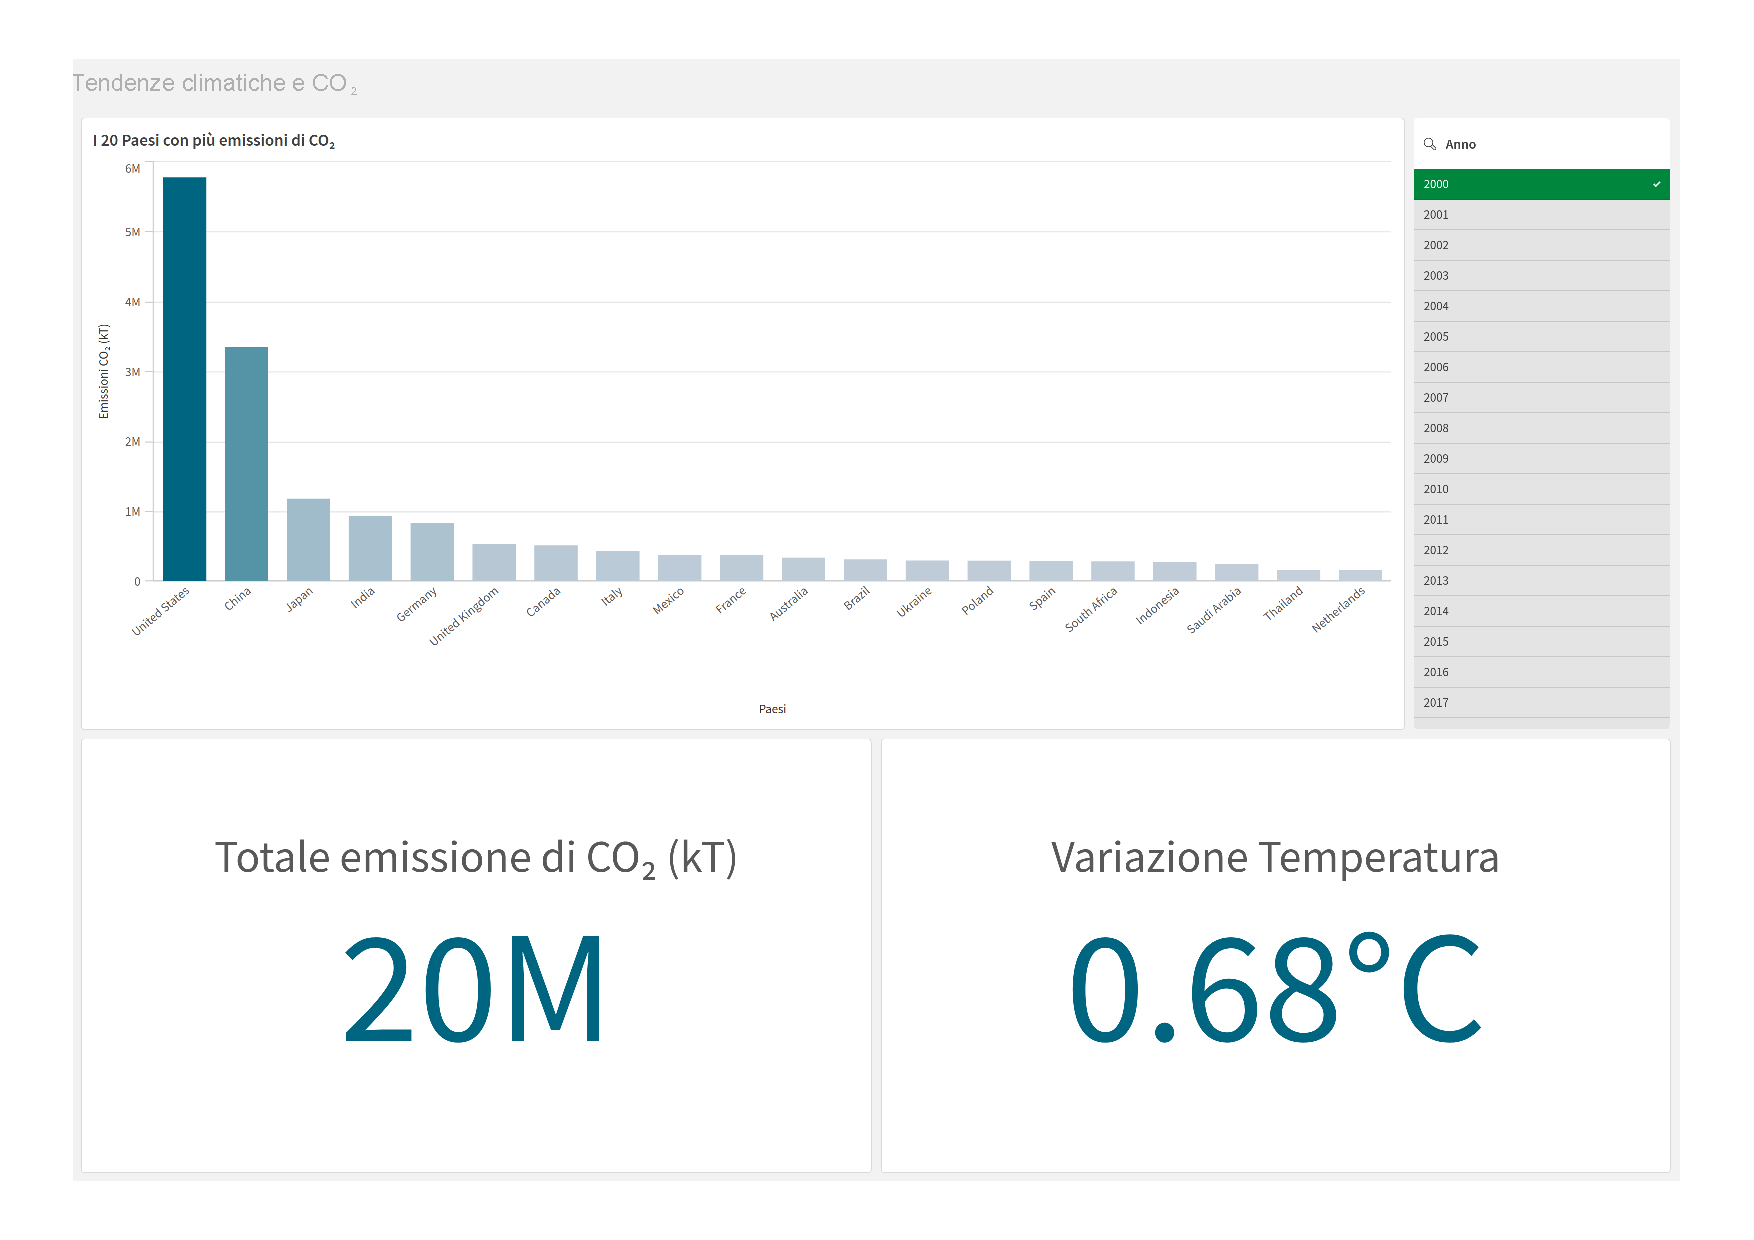
\includegraphics[width=0.7\textwidth]{capitolo_2/img2/4.1 Analisi anno 2000.pdf} \\  % Prima riga
    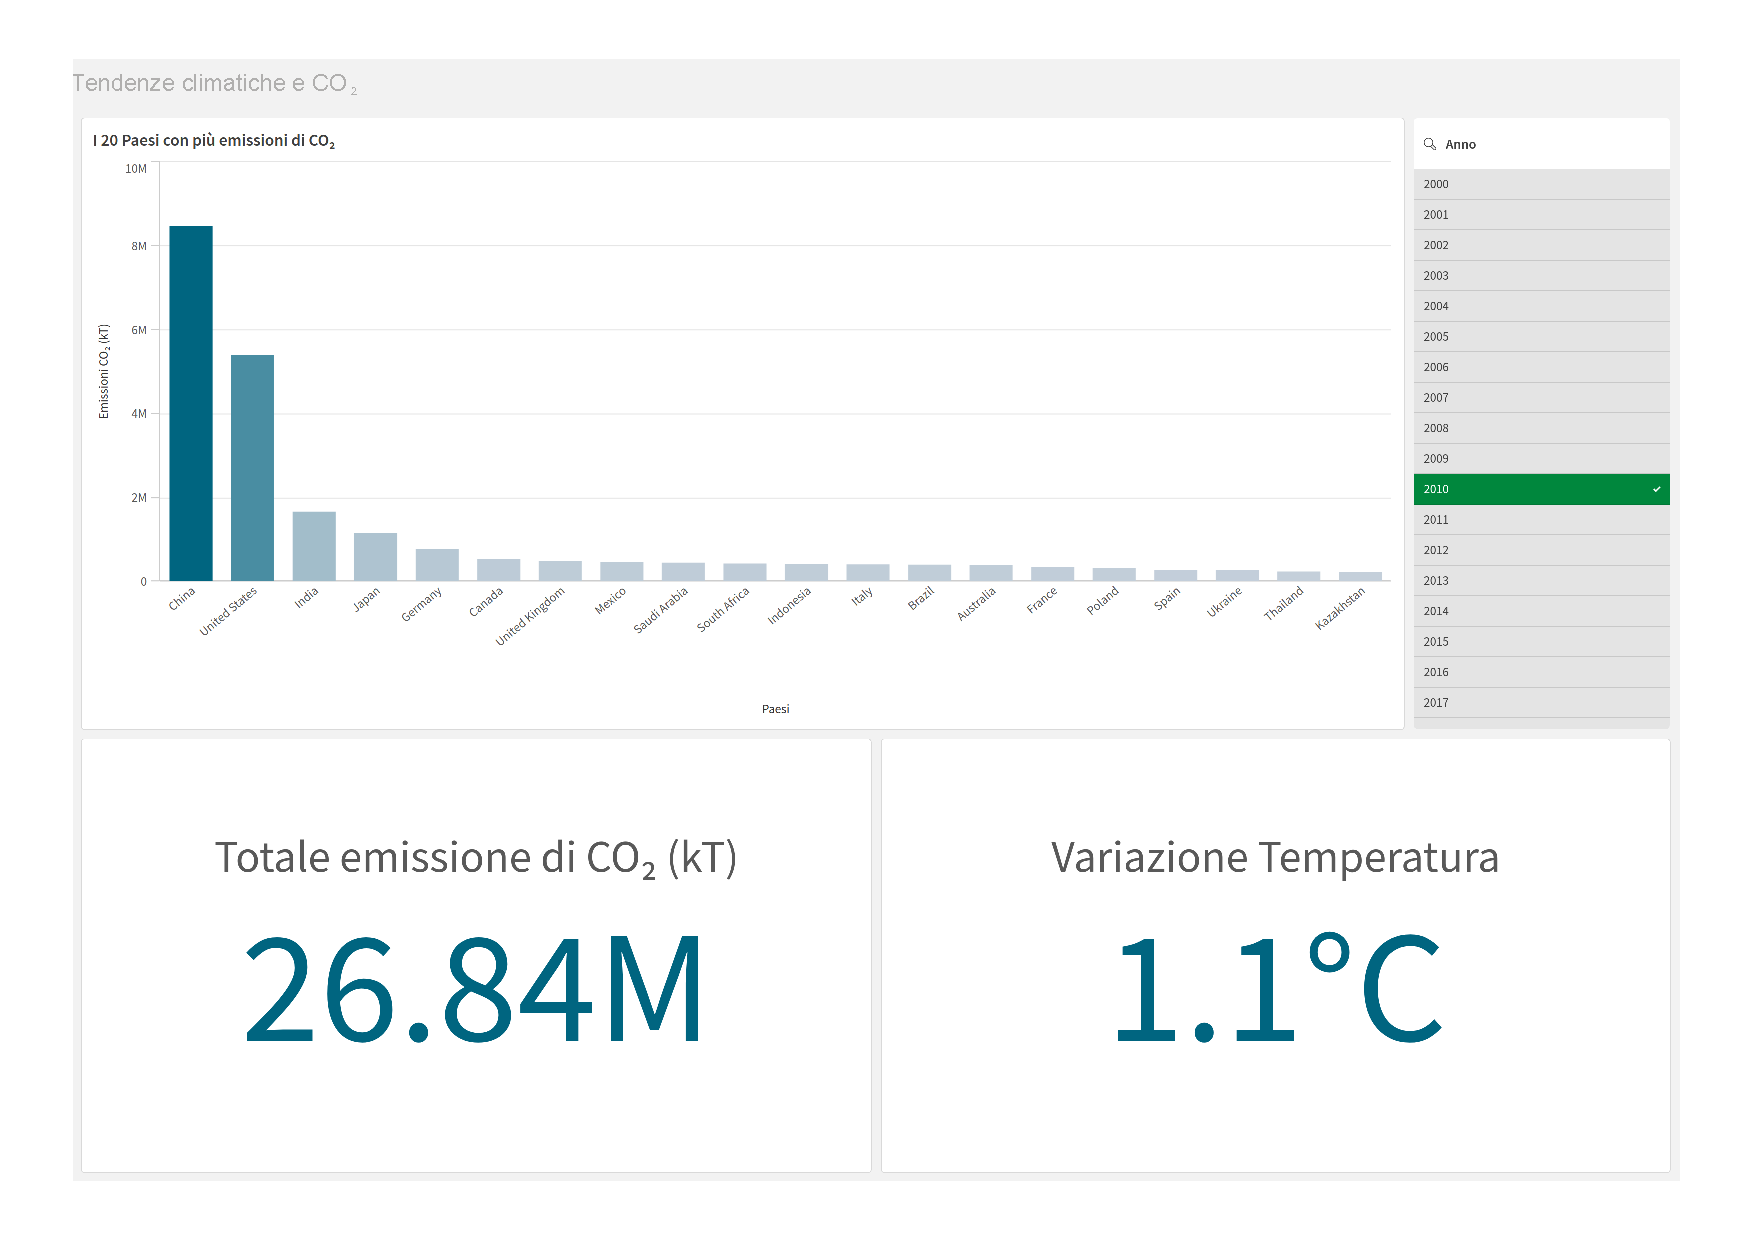
\includegraphics[width=0.7\textwidth]{capitolo_2/img2/4.2 Analisi anno 2010.pdf} \\  % Seconda riga
    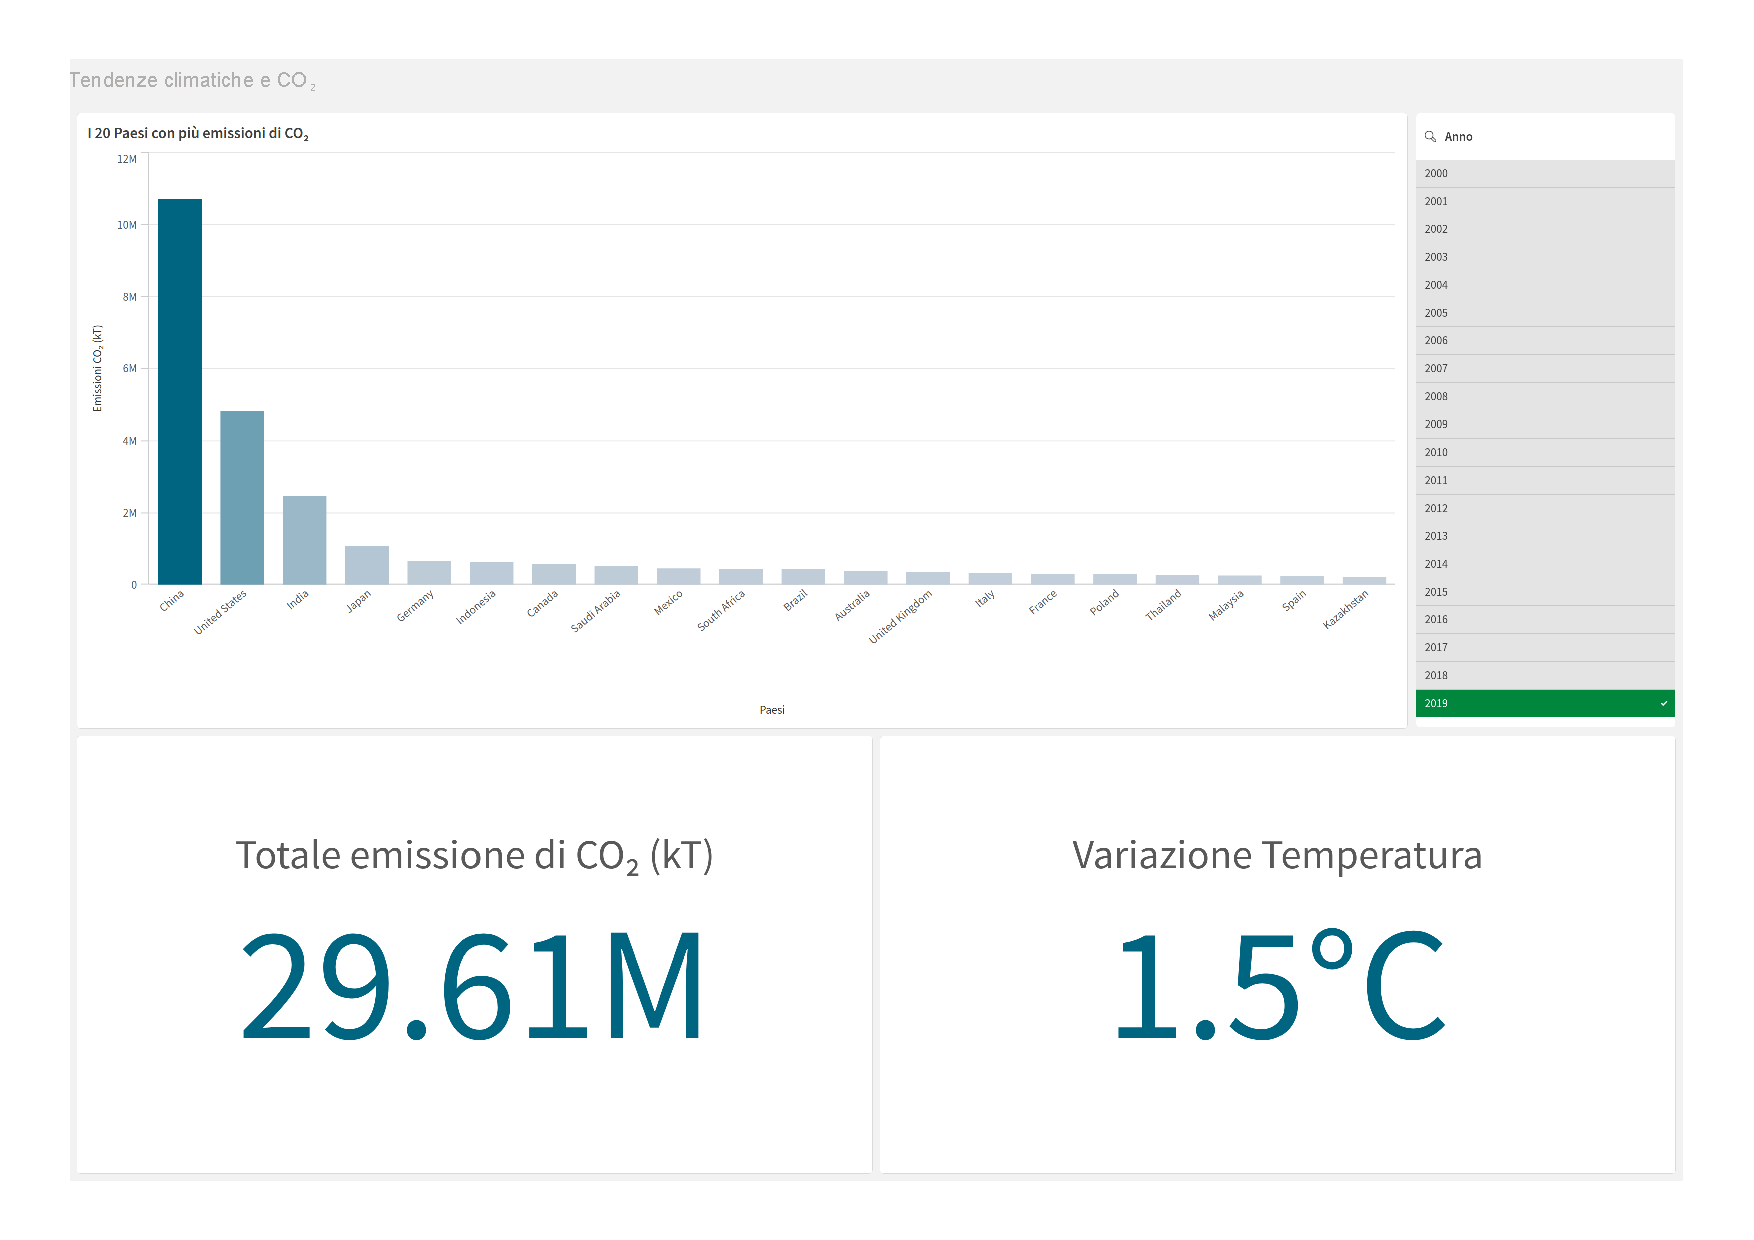
\includegraphics[width=0.7\textwidth]{capitolo_2/img2/4.3 Analisi anno 2019.pdf} \\  % Terza riga
  \end{tabular}
  \caption{Tendenze Climatiche e CO\textsubscript{2}, Anni 2000-2010-2019}
  \label{CO2}
\end{figure}

\subsection{Panorama dell'energia rinnovabile}
La Dashboard, rappresentata in Figura \ref{fig:5.0}, fornisce una panoramica dettagliata sull'impiego delle energie rinnovabili nei diversi Paesi del mondo, consentendo un'analisi approfondita delle tendenze e delle variazioni nel tempo.

Per la sua realizzazione, sono stati utilizzati e integrati due dataset: \textbf{FAOSTAT Temperature Change} e \textbf{Global Data on Sustainable Energy (2000-2020)}.  L’integrazione di queste fonti consente di delineare un quadro esaustivo dell’interazione tra il cambiamento climatico e lo sviluppo delle energie sostenibili, offrendo strumenti analitici utili per supportare decisioni strategiche e la definizione di politiche energetiche a livello internazionale.

\begin{figure}[H]
    \centering
    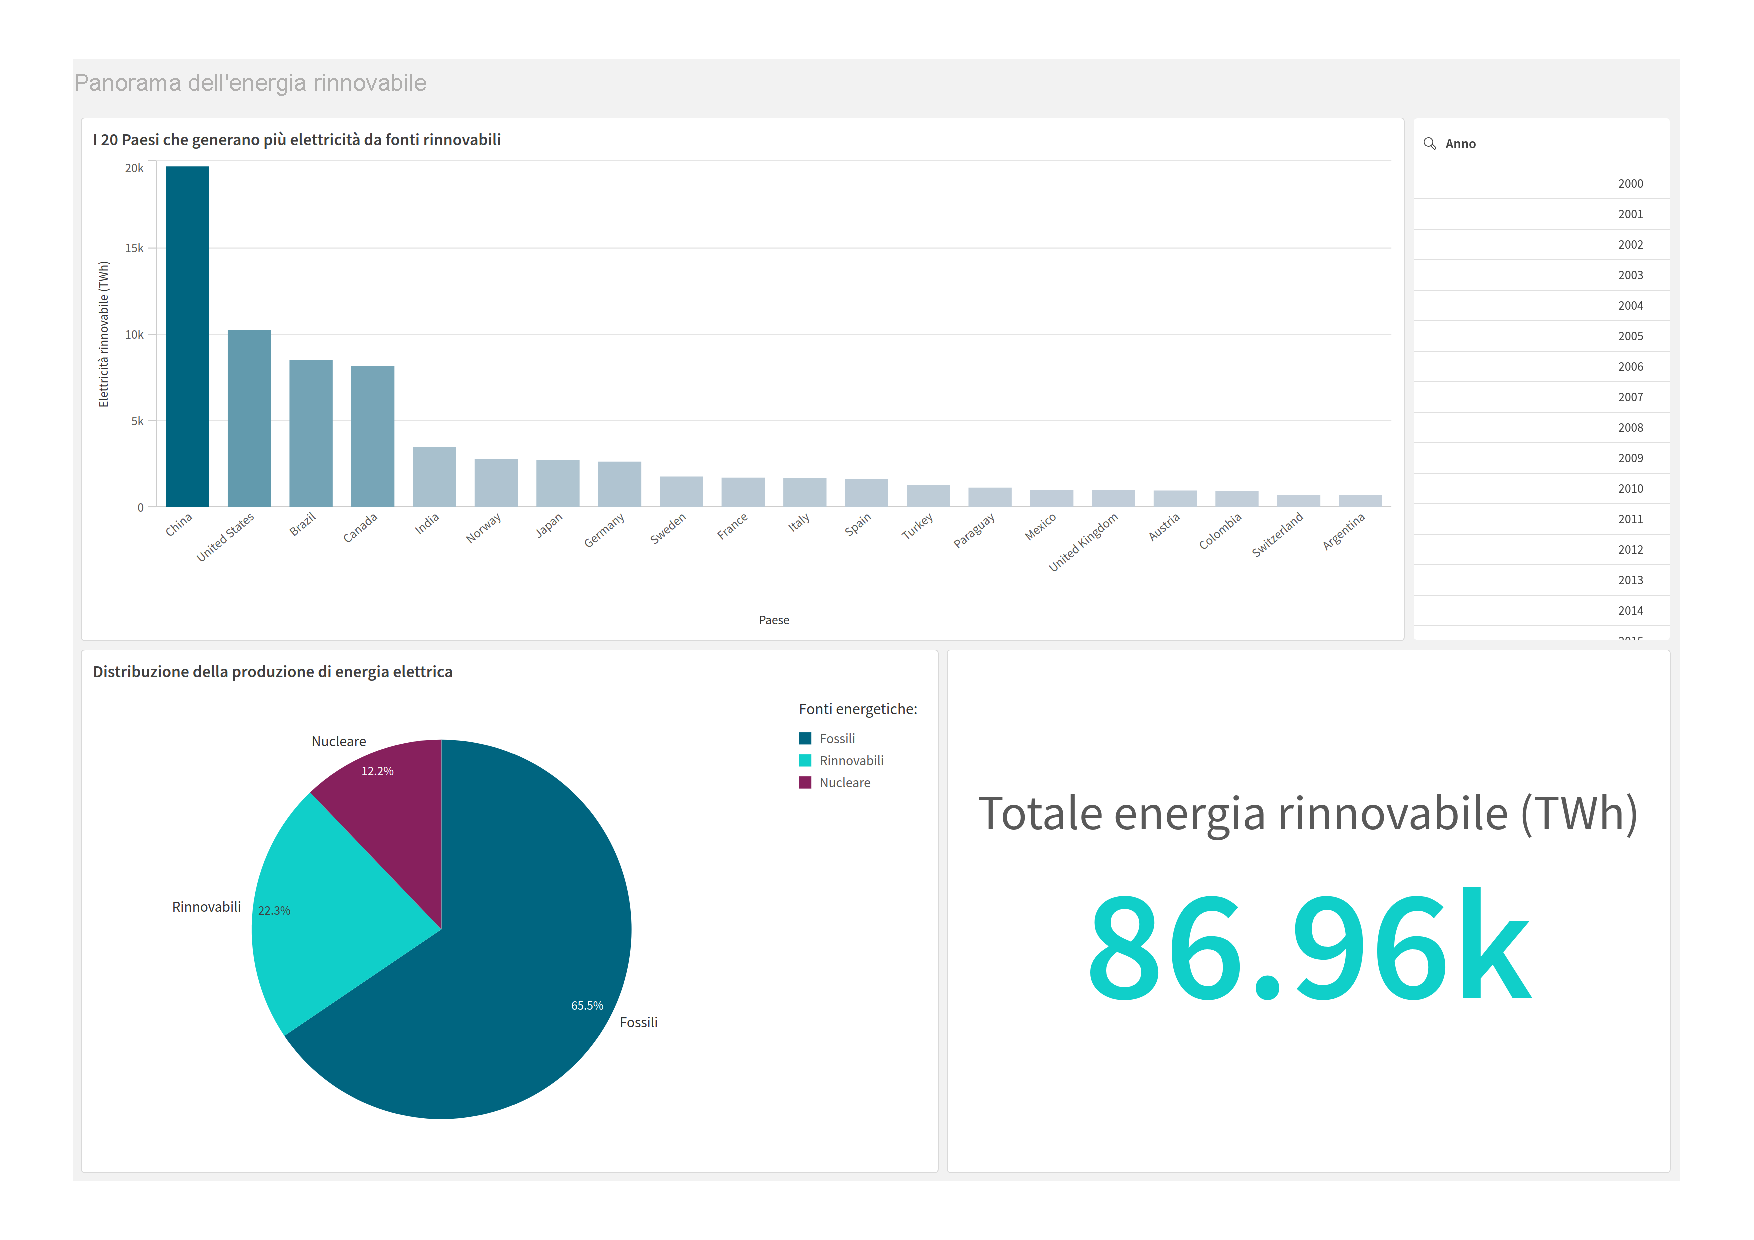
\includegraphics[width=0.98\linewidth]{capitolo_2/img2/5.0 Analisi generale tutti gli anni.pdf}
    \caption{Panorama dell'energia rinnovabile}
    \label{fig:5.0}
\end{figure}

\subsubsection{Struttura Dashboard}
La struttura della Dashboard è organizzata in diverse sezioni, ciascuna delle quali fornisce informazioni dettagliate sull'impiego delle energie rinnovabili a livello globale attraverso rappresentazioni grafiche e indicatori chiave di performance.  

Nella parte superiore sinistra della Dashboard è presente il grafico \textbf{I 20 Paesi che generano più elettricità da fonti rinnovabili}, che classifica le nazioni in base alla quantità di energia elettrica prodotta tramite fonti rinnovabili. Questo grafico consente di identificare i Paesi leader nel settore dell'energia sostenibile, evidenziando quelli che hanno investito maggiormente nelle tecnologie rinnovabili e confrontando il loro posizionamento rispetto ad altre nazioni.  

Nella parte inferiore sinistra, si trova il diagramma a torta \textbf{Distribuzione della produzione di energia elettrica}, il quale rappresenta graficamente la ripartizione percentuale delle diverse fonti energetiche impiegate nella generazione di elettricità. Grazie a questa visualizzazione, è possibile comprendere in che misura ciascuna fonte contribuisce al panorama energetico complessivo e valutare il peso specifico delle rinnovabili rispetto alle fonti fossili e quelle nucleari.  

Sul lato destro della Dashboard è posizionato un KPI denominato \textbf{Totale energia rinnovabile (TWh)}, che evidenzia il quantitativo complessivo di energia rinnovabile prodotta a livello internazionale. Questo indicatore consente di monitorare l'andamento della produzione di energia sostenibile nel tempo, facilitando confronti tra diversi periodi e supportando l'analisi dell'efficacia delle politiche energetiche adottate dai vari Paesi.  

Inoltre, la Dashboard offre la possibilità di applicare filtri temporali, consentendo agli utenti di selezionare specifici intervalli di anni per analizzare l'evoluzione della produzione di energia rinnovabile in determinati periodi. Questa funzionalità permette di individuare tendenze, valutare l'impatto delle strategie adottate nel tempo e ottenere una visione più approfondita dell'evoluzione del settore energetico sostenibile su scala globale.

\subsubsection{Obiettivo dell'Analisi}
Questa Dashboard è stata progettata con l’obiettivo di offrire uno strumento interattivo e approfondito per l'analisi dell'impiego delle energie rinnovabili nei Paesi oggetto di studio, nel periodo compreso tra il 2000 e il 2019. Grazie alla sua struttura dinamica, consente agli utenti di esplorare in dettaglio l'evoluzione dell'adozione delle fonti energetiche sostenibili, fornendo un supporto visivo chiaro e intuitivo per la comprensione delle tendenze globali.  

Una delle principali funzionalità della Dashboard è la possibilità di selezionare specifici intervalli temporali, come illustrato in Figura \ref{energia}, al fine di analizzare le variazioni nell'utilizzo delle fonti rinnovabili nel corso degli anni. Questo consente di individuare pattern di crescita, momenti di accelerazione o rallentamento nello sviluppo delle energie sostenibili e di correlare tali cambiamenti con fattori economici, politici o tecnologici.  

\begin{myoutline}
    \textbf{Nota}: La scelta degli anni 2000-2010-2019 è motivata dalla volontà di voler esplorare l'andamento complessivo dell'utilizzo delle energie rinnovabili nell'intero periodo considerato.
\end{myoutline}

\begin{figure}[p]
  \centering
  \begin{tabular}{c}  
    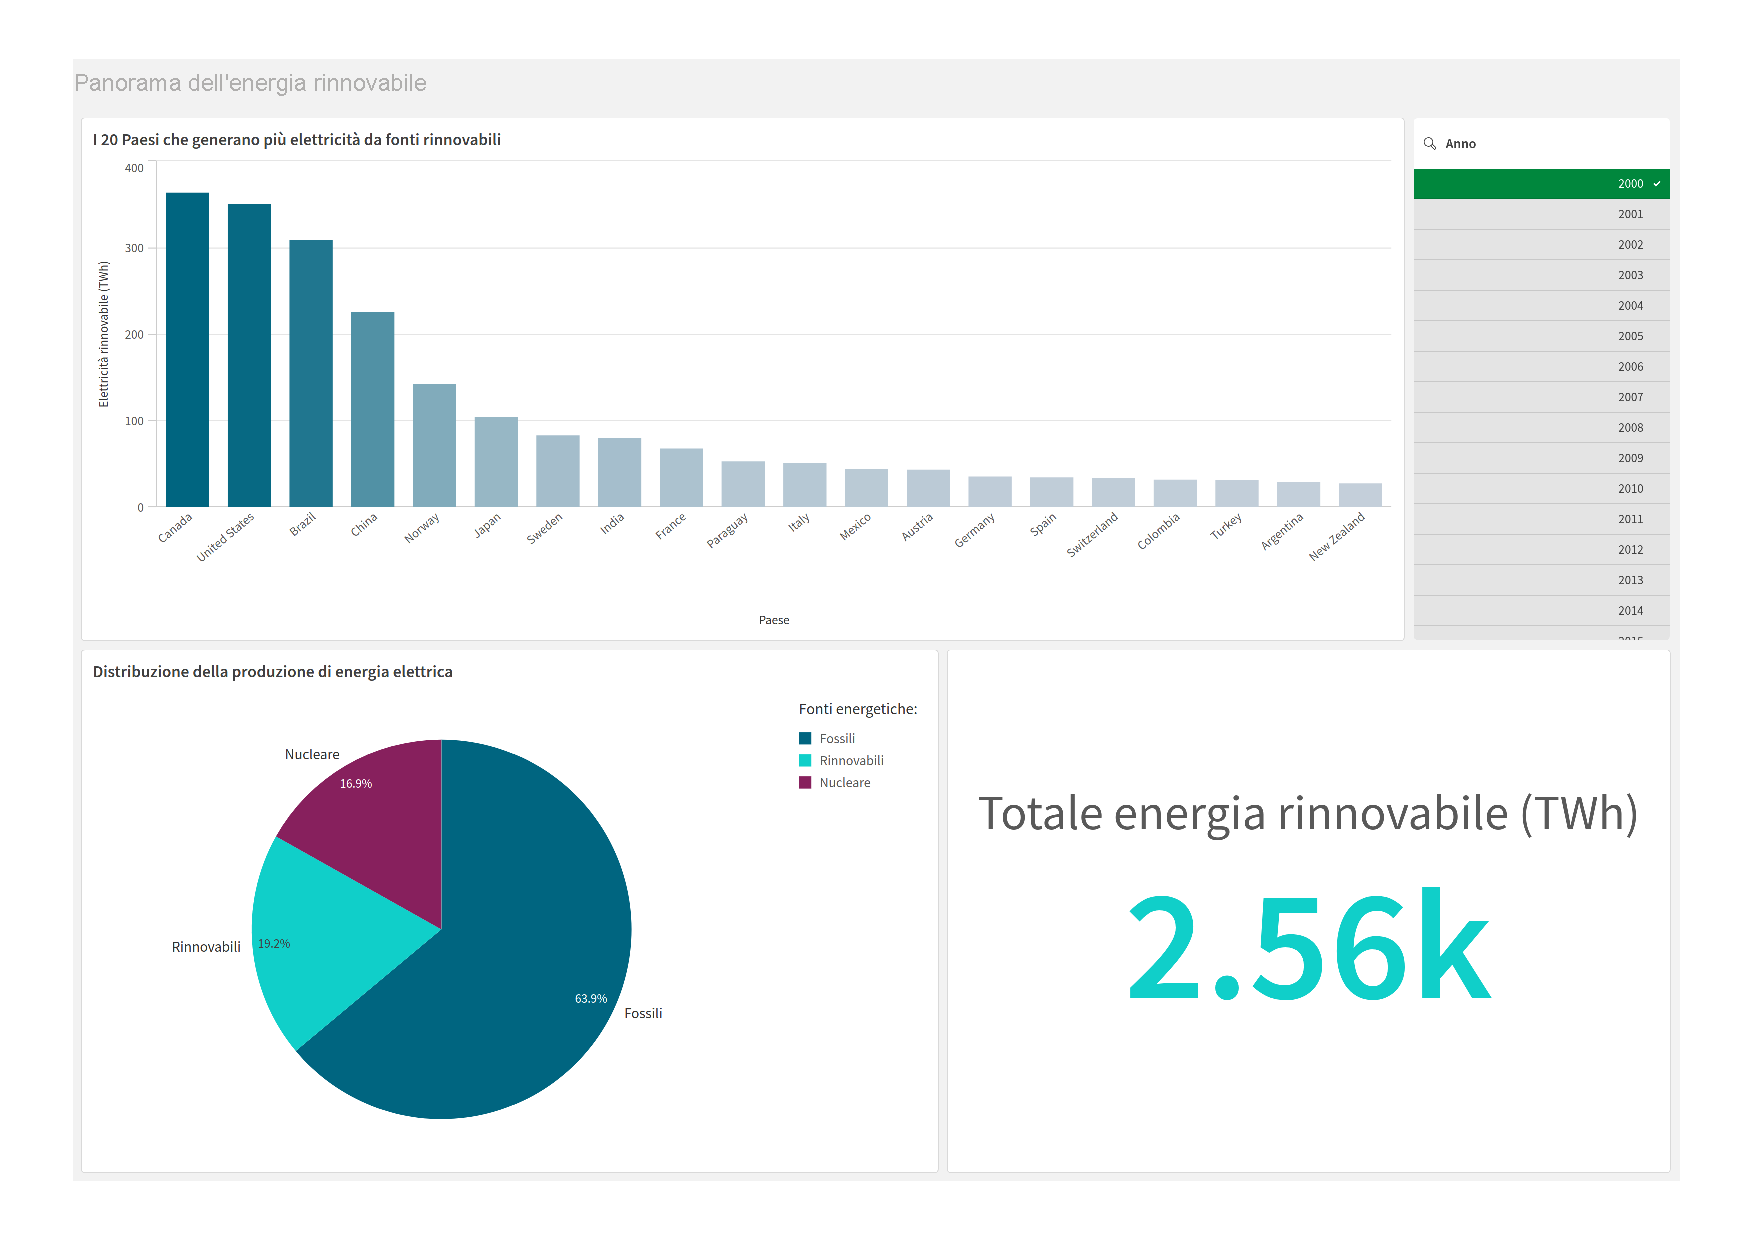
\includegraphics[width=0.7\textwidth]{capitolo_2/img2/5.1 Analisi anno 2000.pdf} \\  % Prima riga
    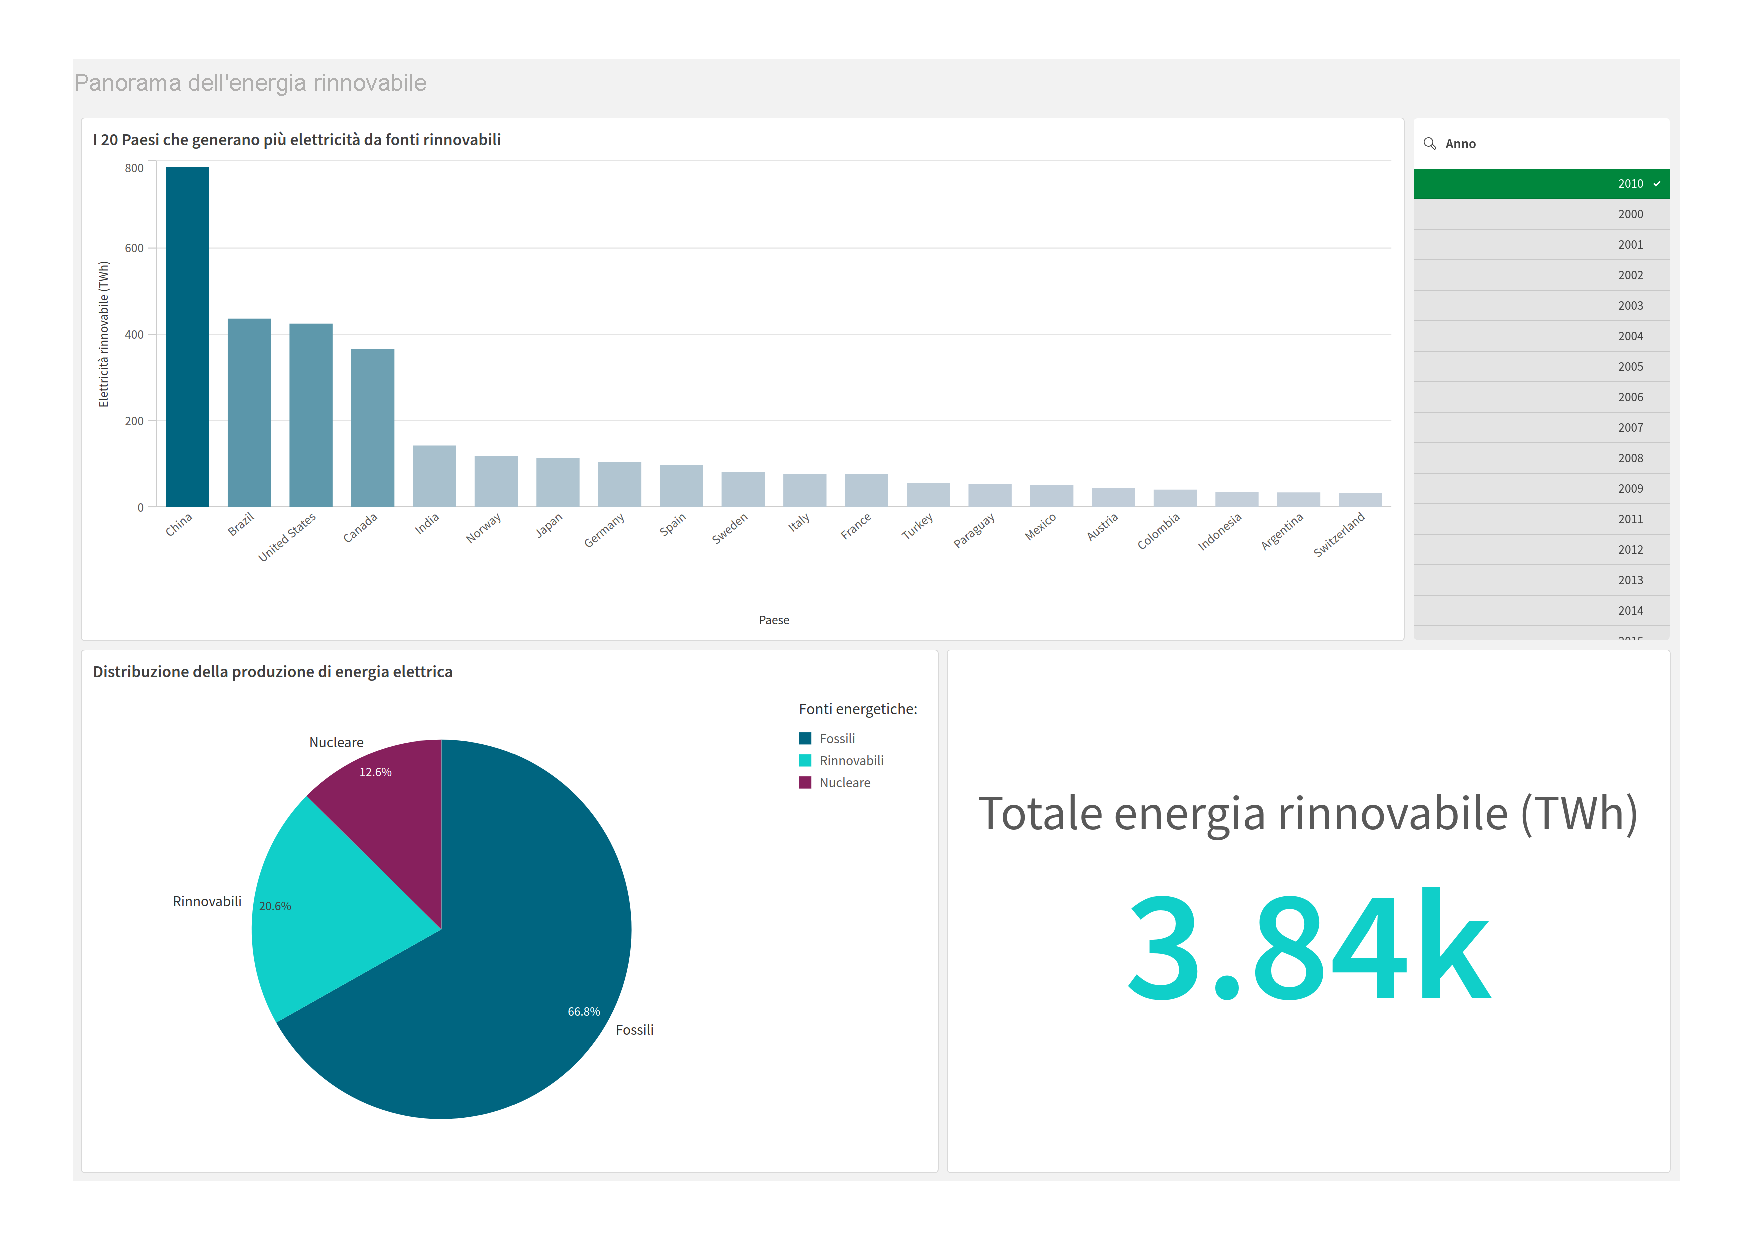
\includegraphics[width=0.7\textwidth]{capitolo_2/img2/5.2 Analisi anno 2010.pdf} \\  % Seconda riga
    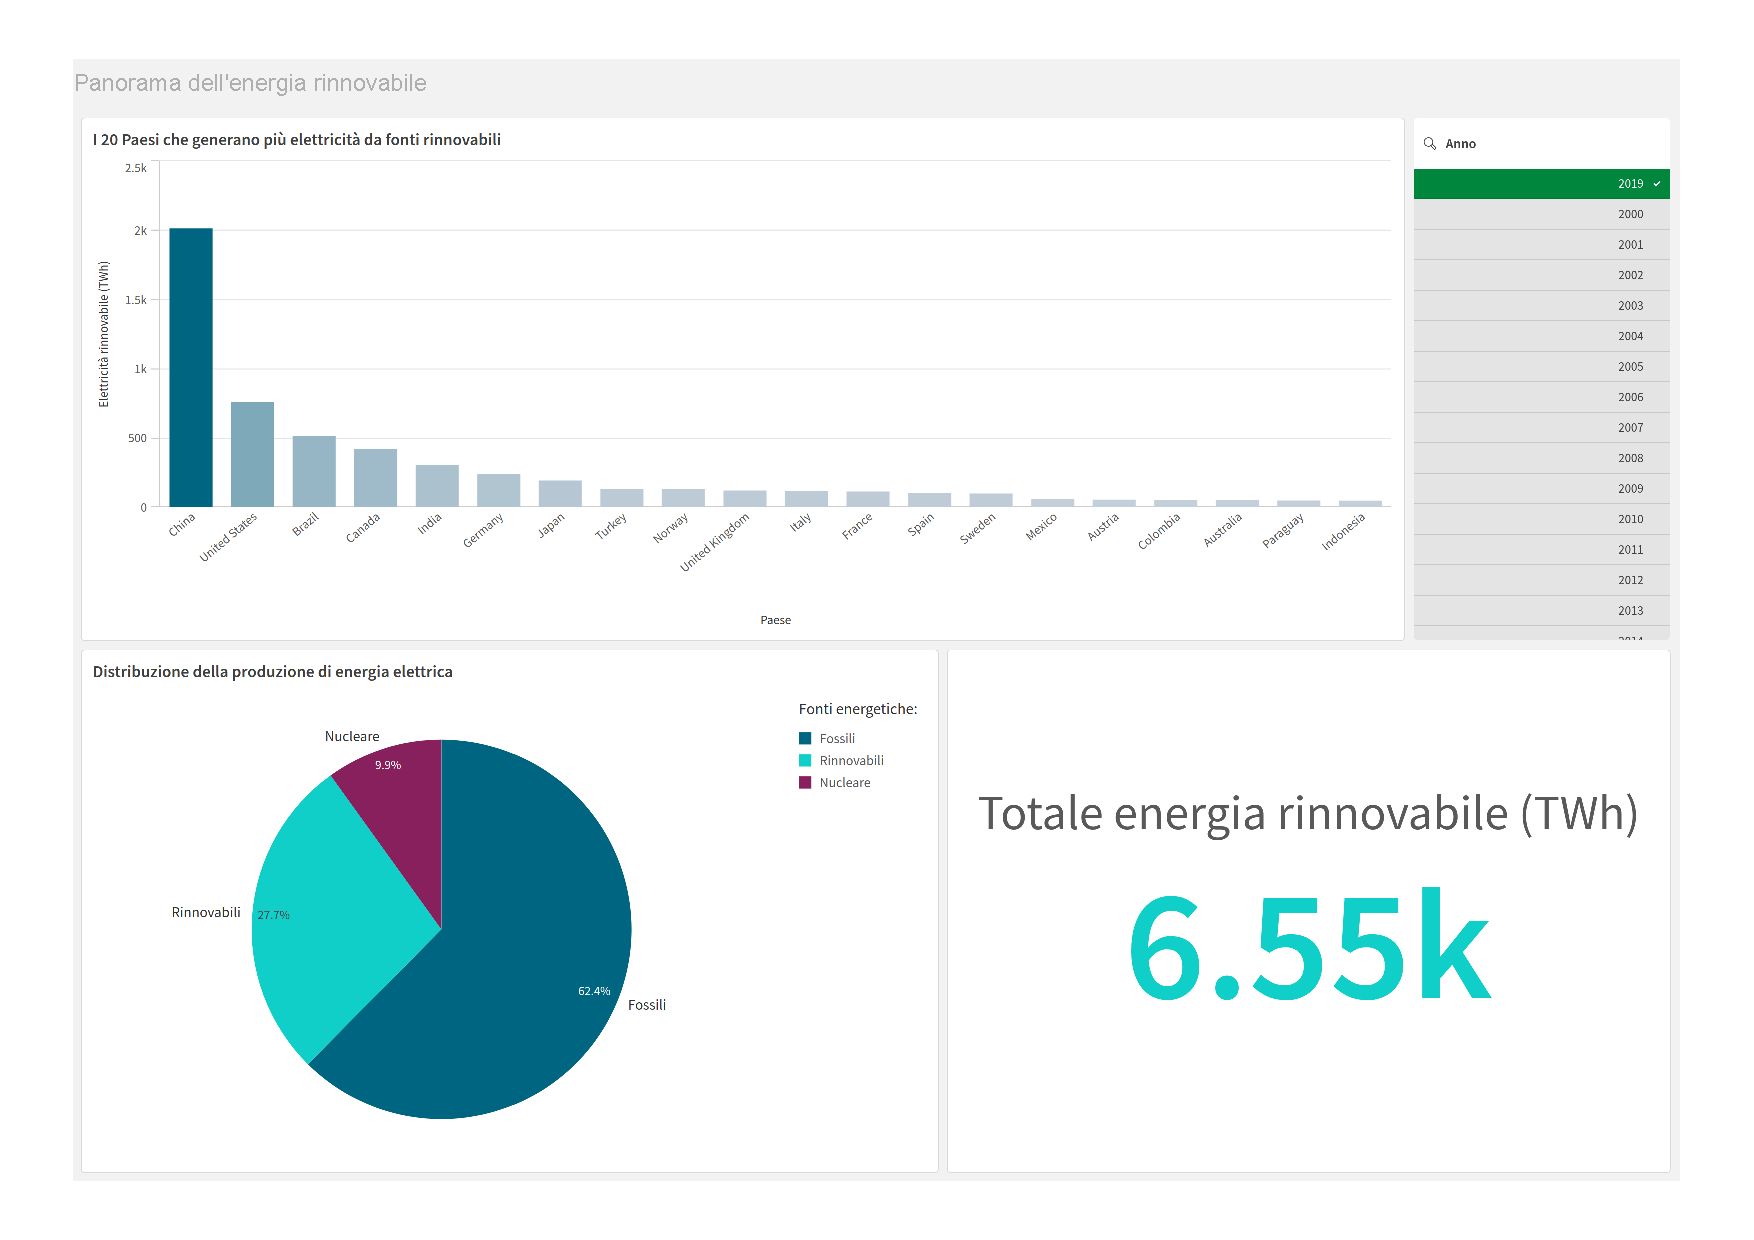
\includegraphics[width=0.7\textwidth]{capitolo_2/img2/5.3 Analisi anno 2019.pdf} \\  % Terza riga
  \end{tabular}
  \caption{Panorama dell'energia rinnovabile, Anni 2000-2010-2019}
  \label{energia}
\end{figure}

\begin{figure}[p]
    \centering
    \subfloat[\textbf{Cina 2000}]{%
        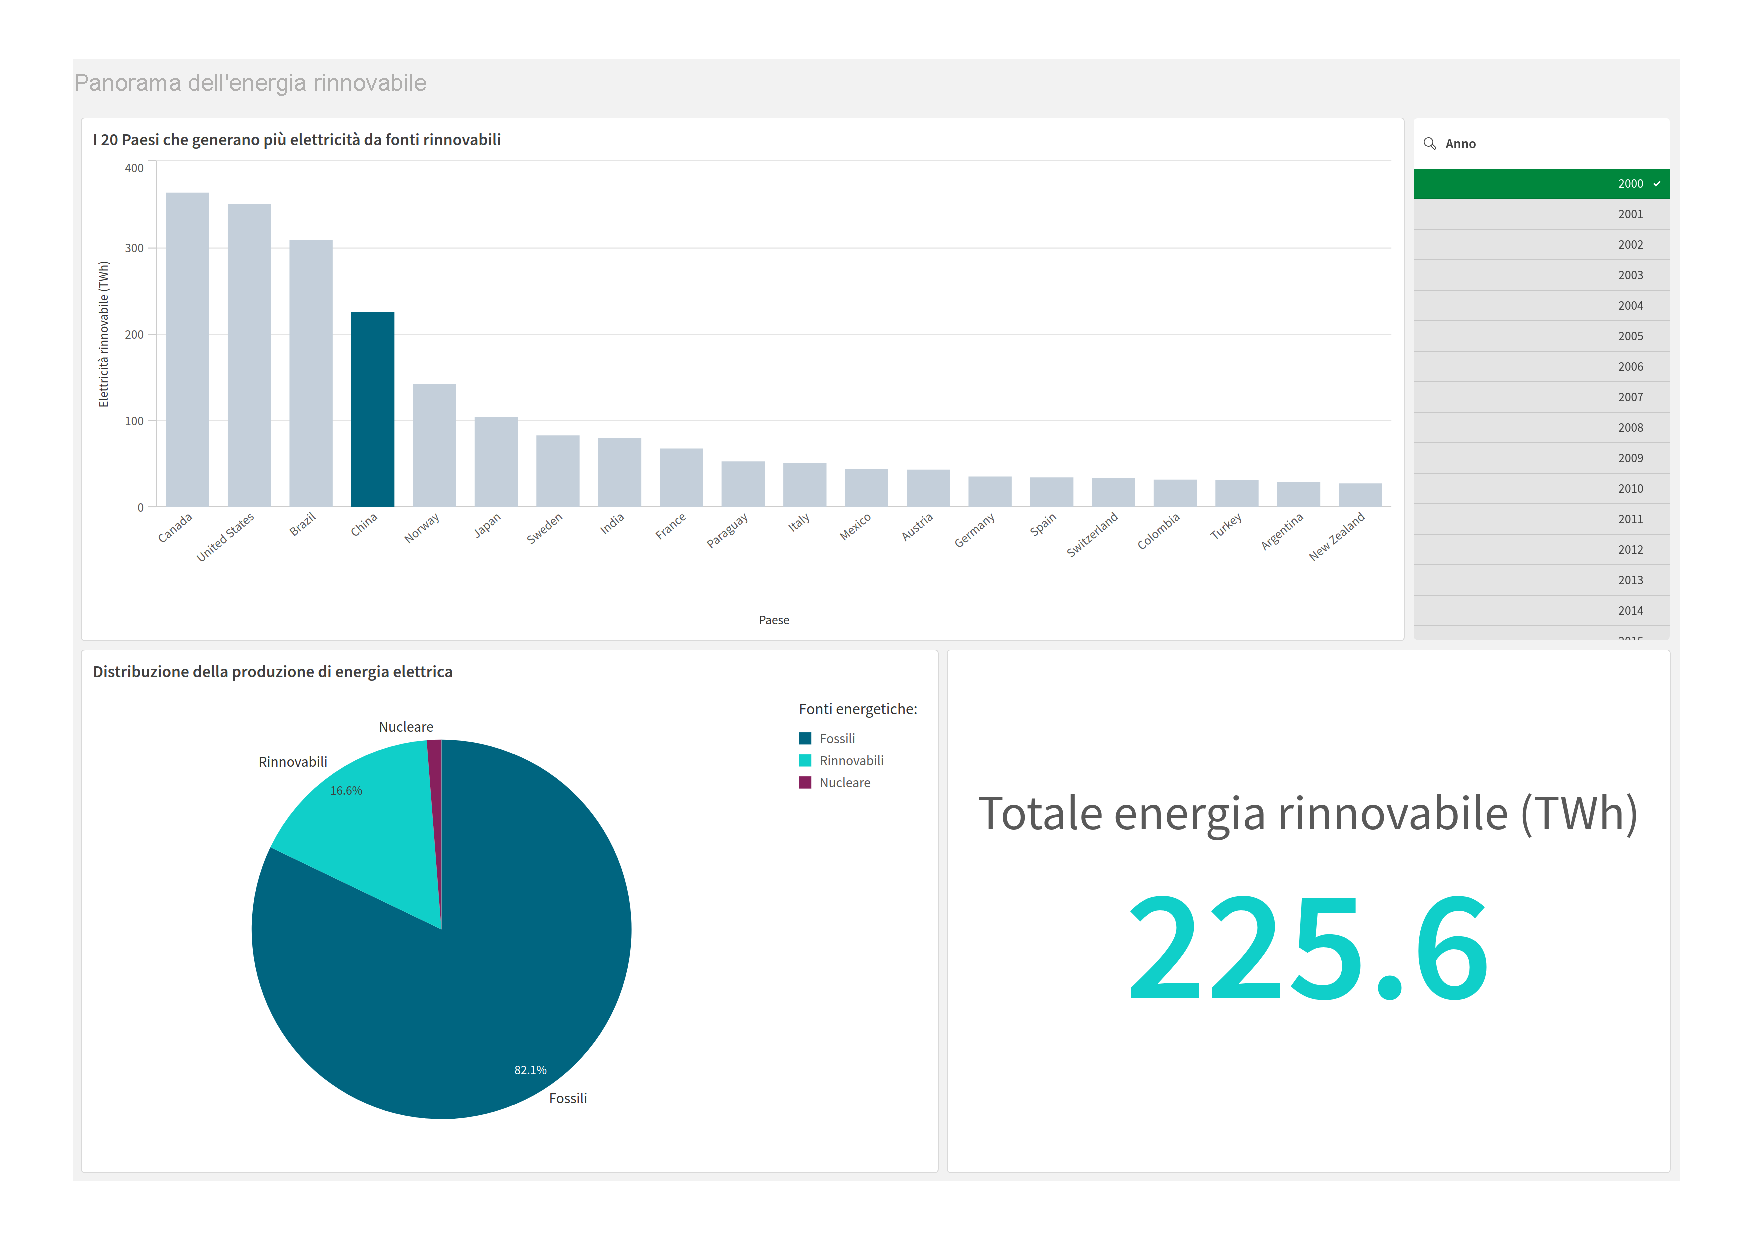
\includegraphics[width=0.50\textwidth]{capitolo_2/img2/5.4.1 Analisi Cina 2000.pdf}}
    \hfill
    \subfloat[\textbf{USA 2000}]{%
        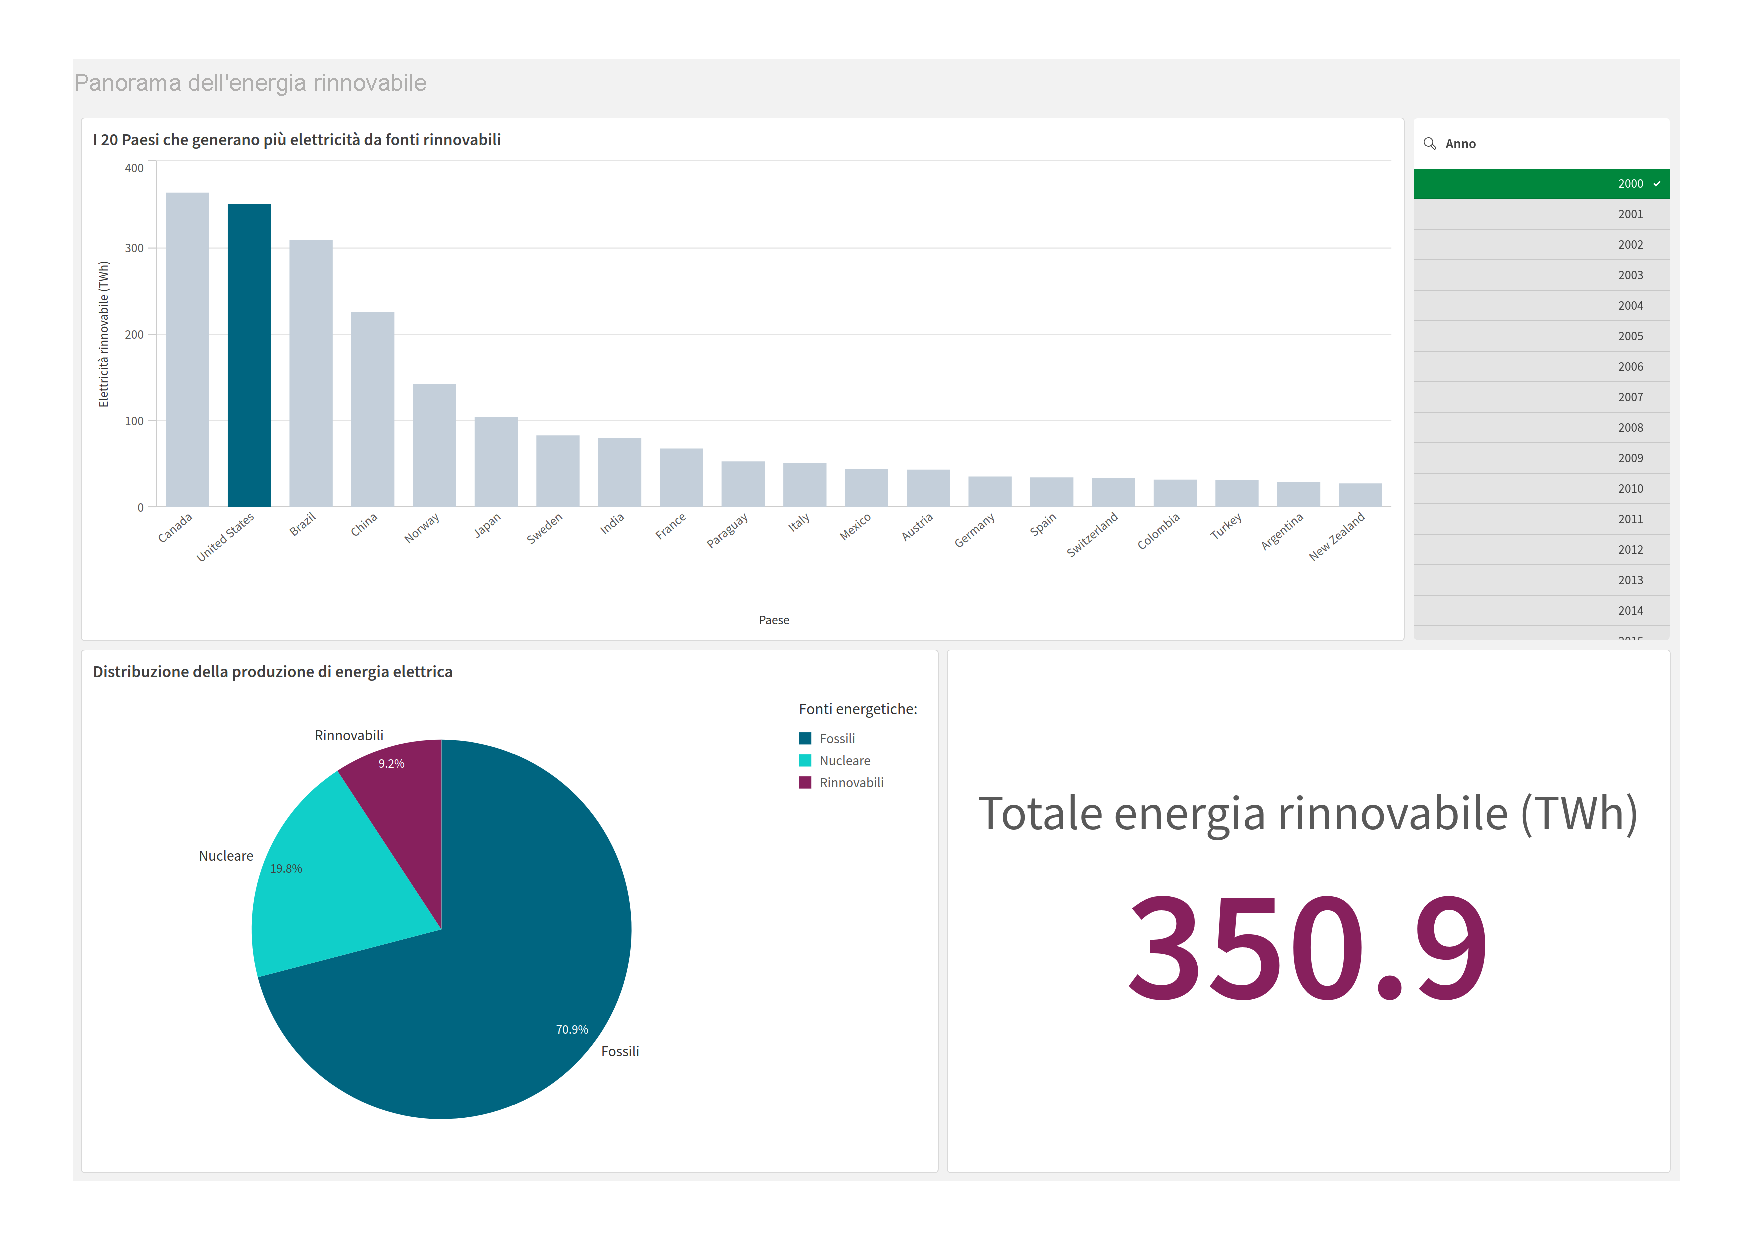
\includegraphics[width=0.50\textwidth]{capitolo_2/img2/5.5.1 Analisi USA 2000.pdf}} \\
    
    \subfloat[\textbf{Cina 2010}]{%
        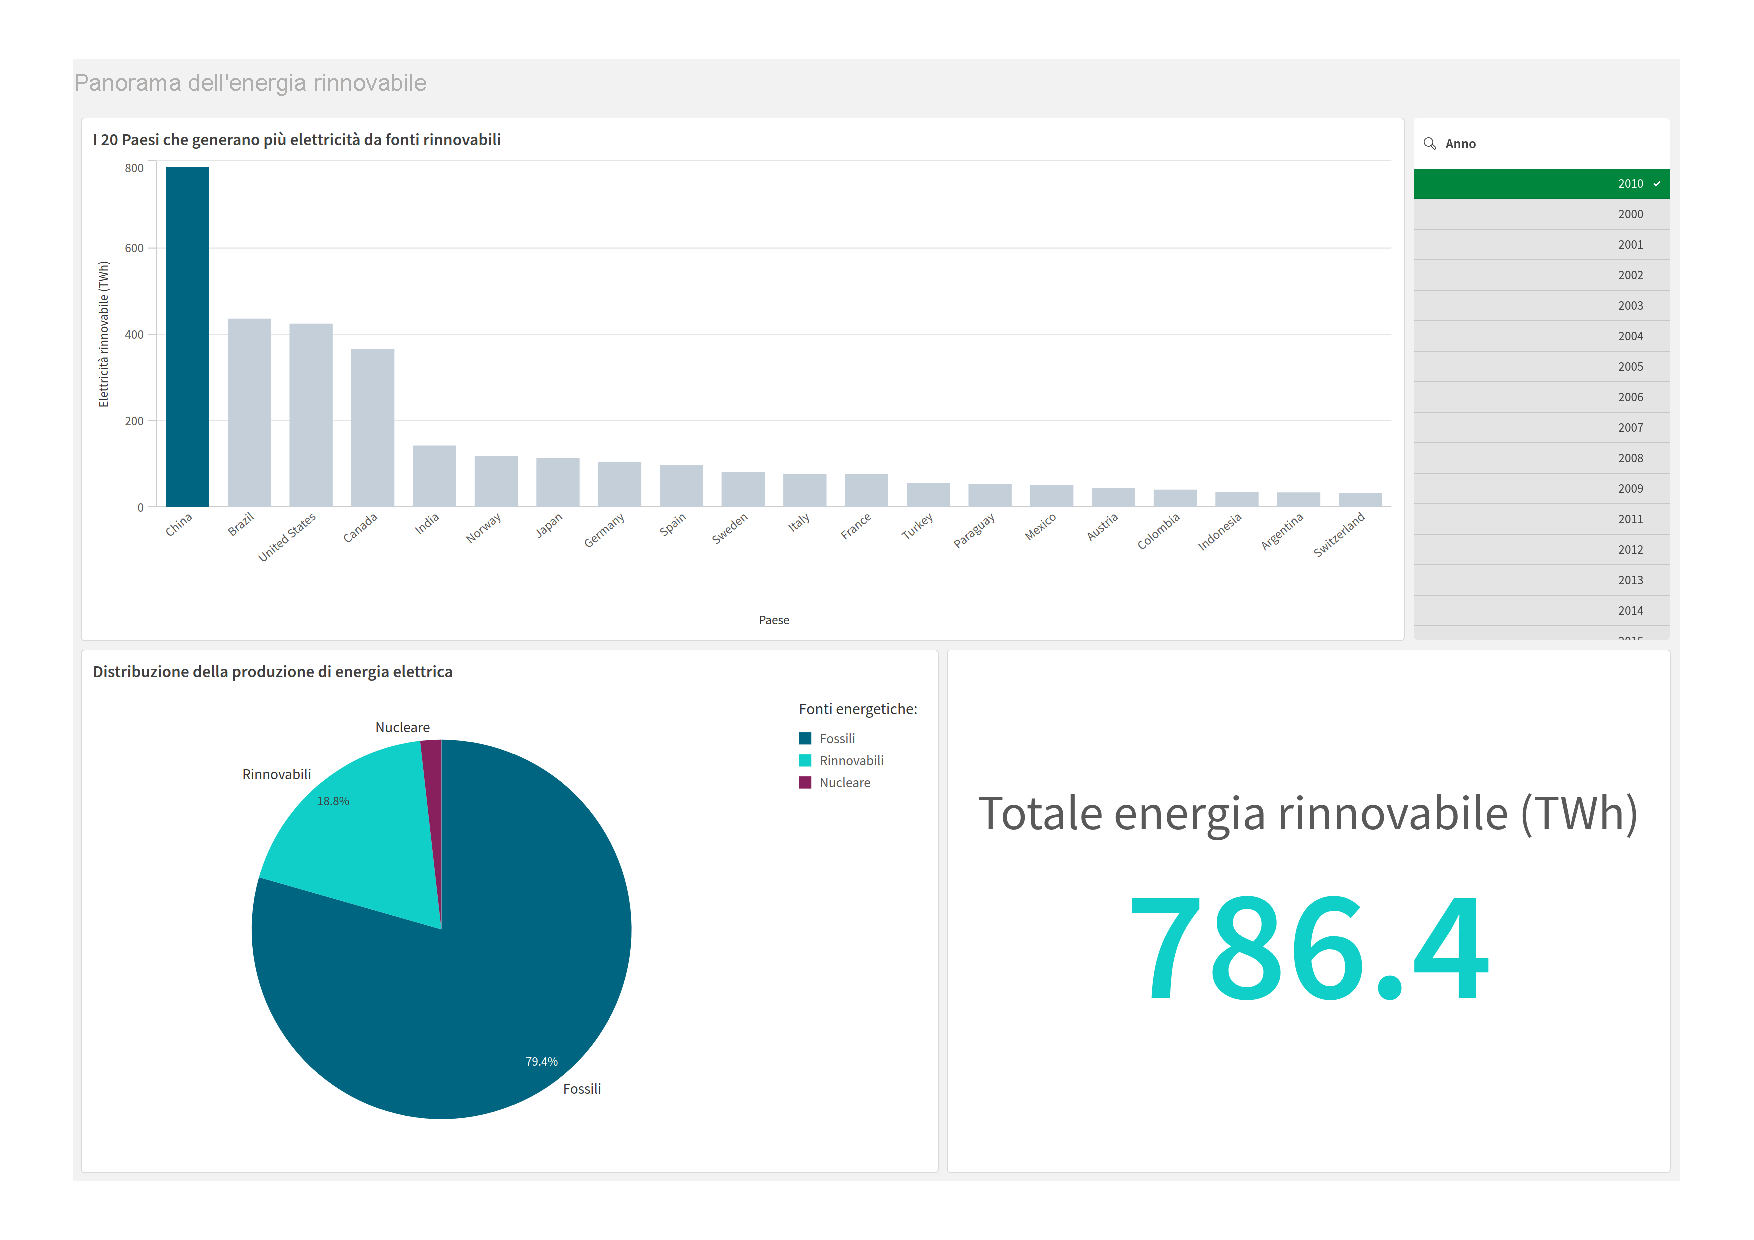
\includegraphics[width=0.50\textwidth]{capitolo_2/img2/5.4.2 Analisi Cina 2010.pdf}}
    \hfill
    \subfloat[\textbf{USA 2010}]{%
        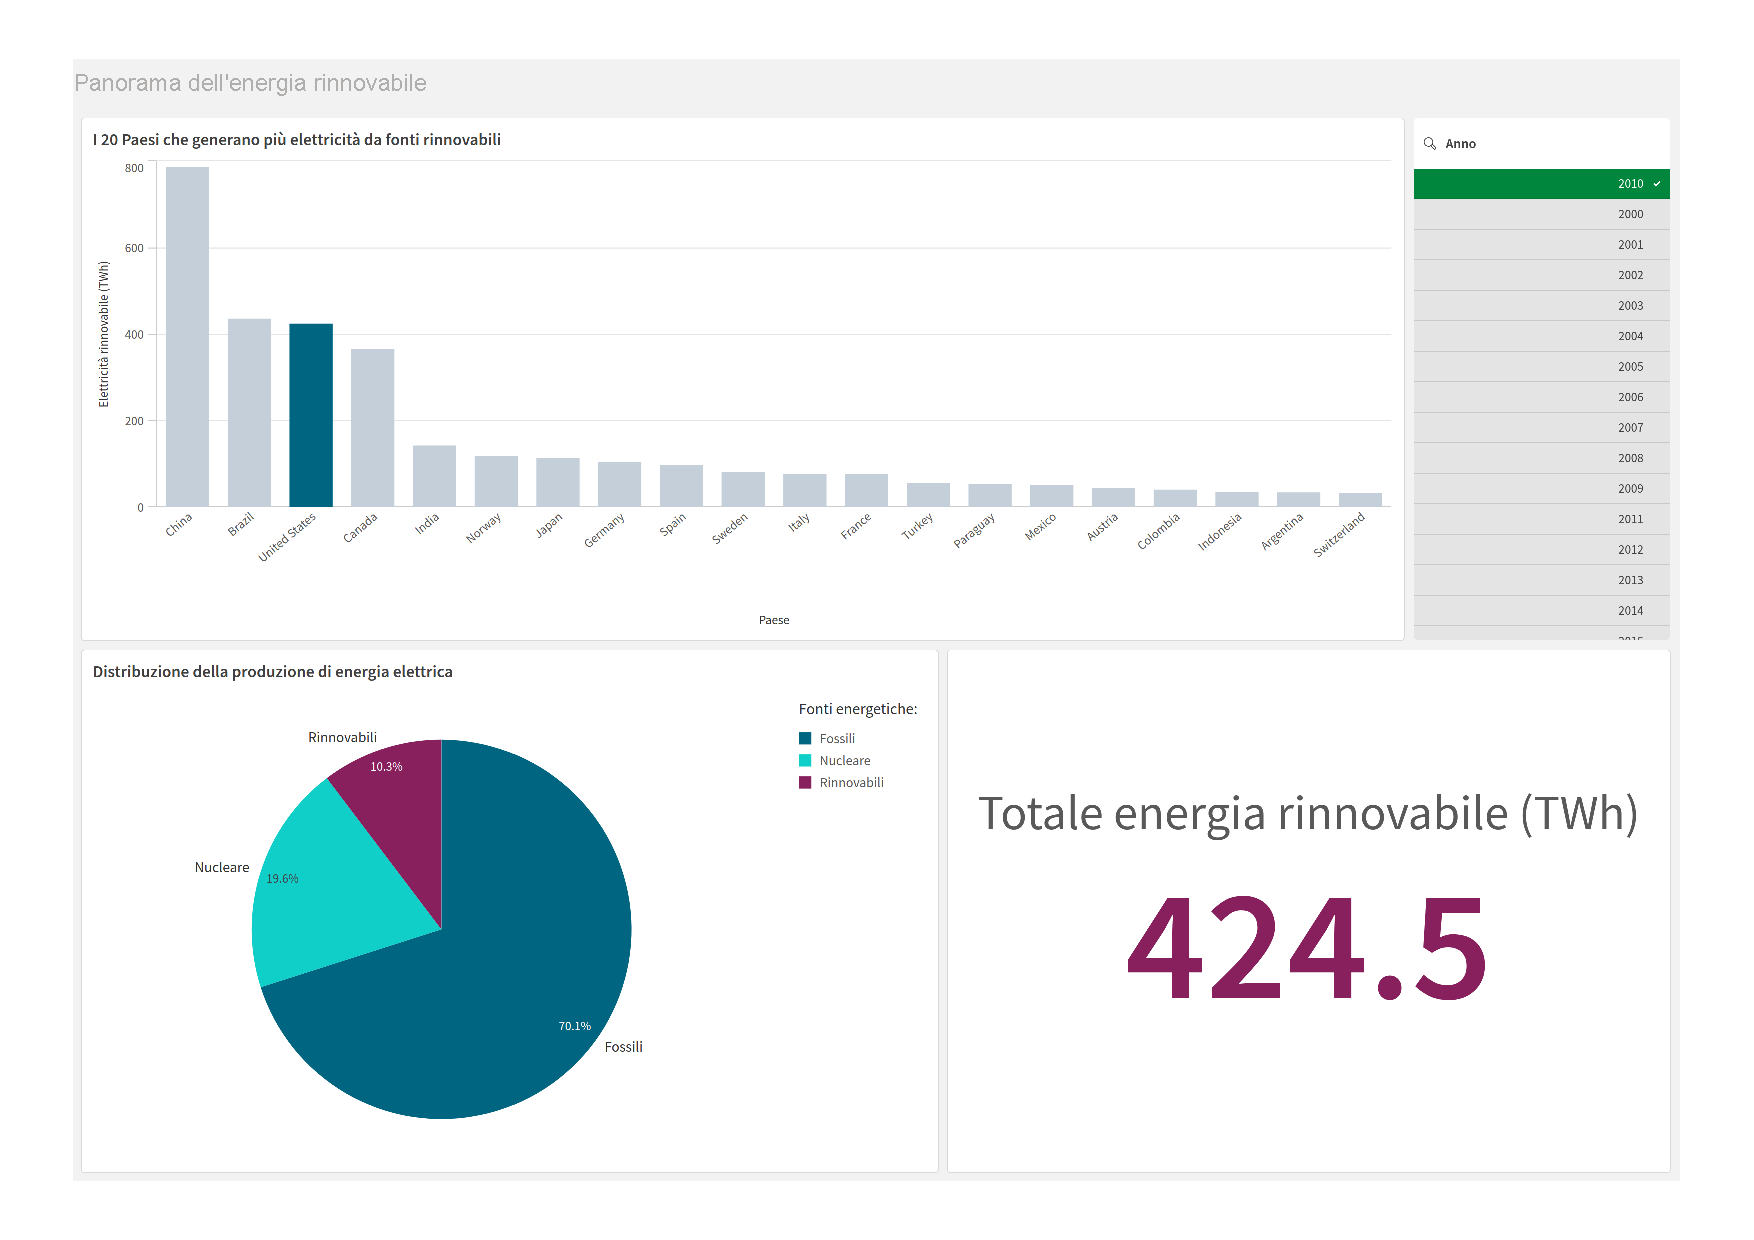
\includegraphics[width=0.50\textwidth]{capitolo_2/img2/5.5.2 Analisi USA 2010.pdf}} \\
    
    \subfloat[\textbf{Cina 2019}]{%
        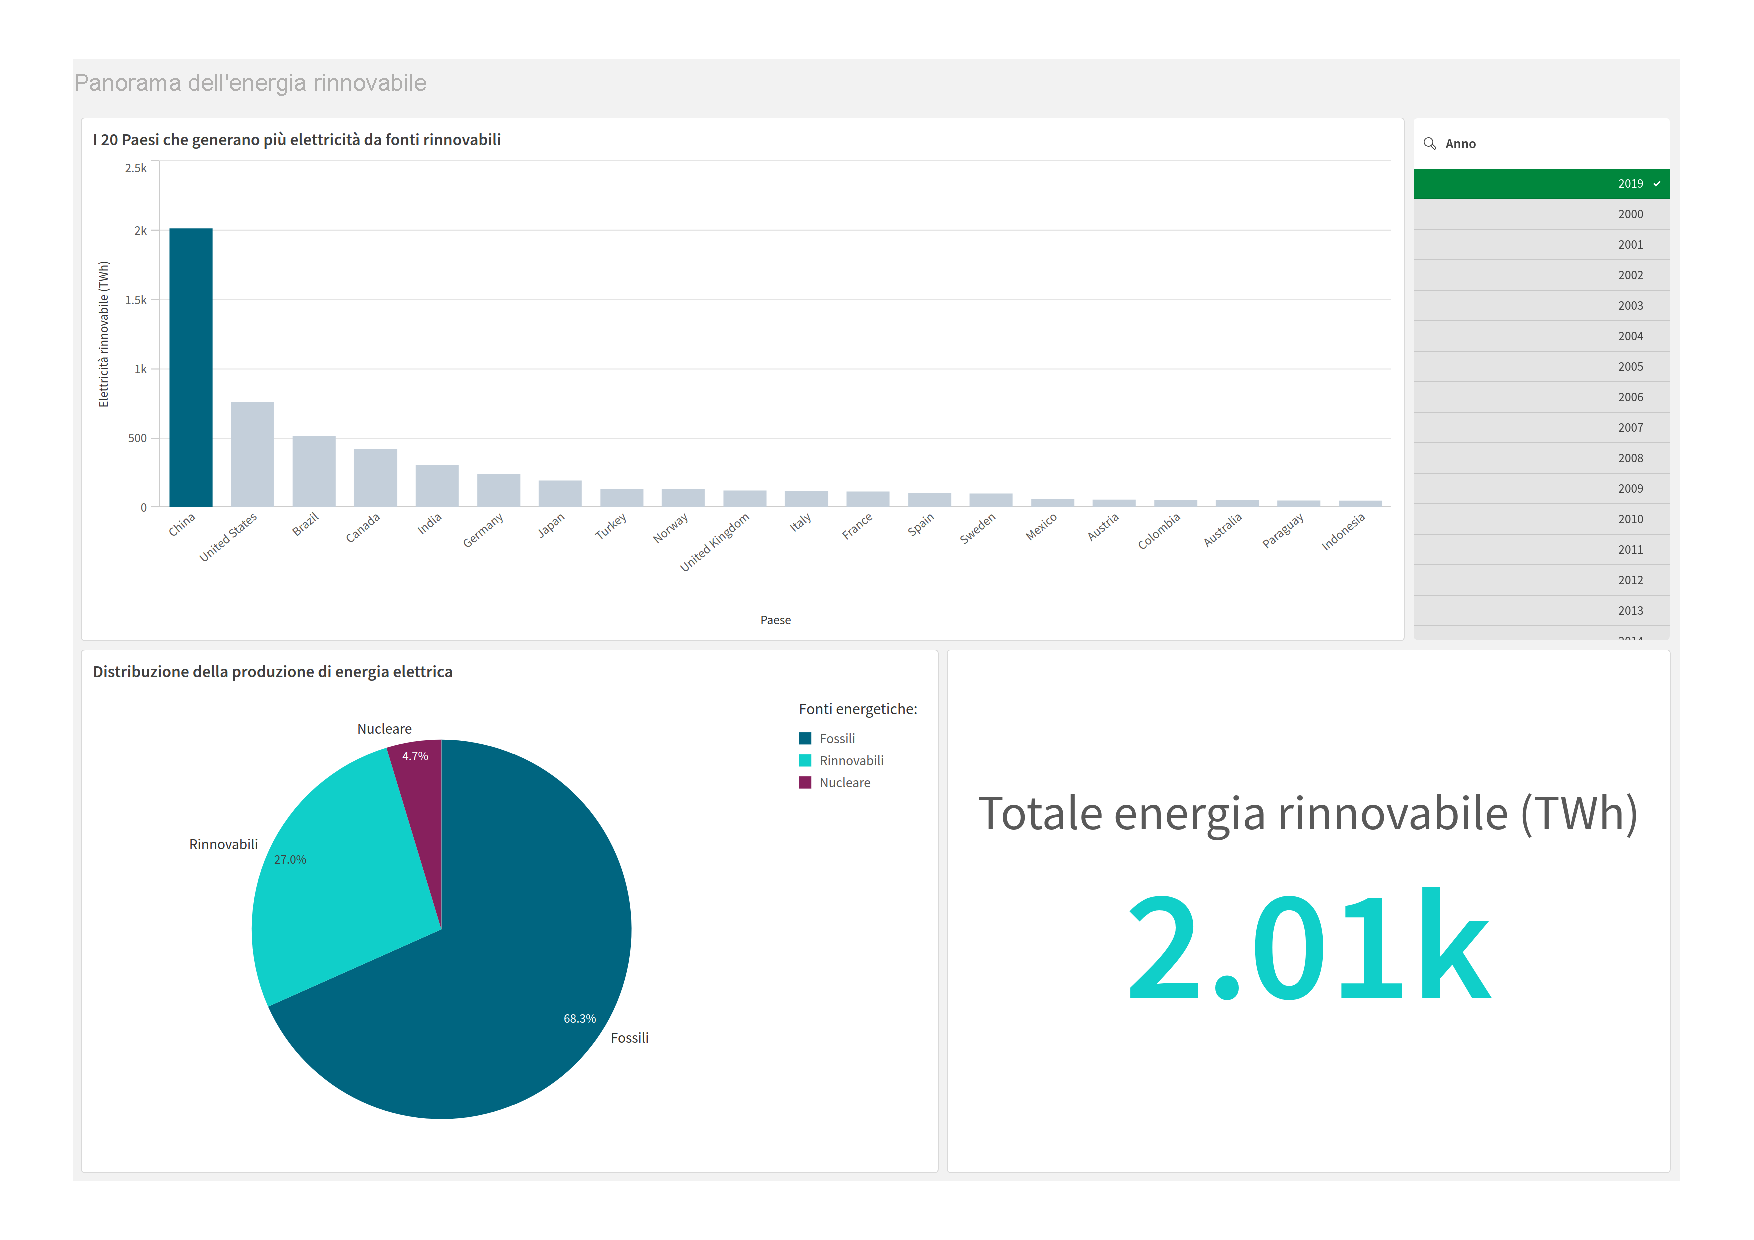
\includegraphics[width=0.50\textwidth]{capitolo_2/img2/5.4.3 Analisi Cina 2019.pdf}}
    \hfill
    \subfloat[\textbf{USA 2019}]{%
        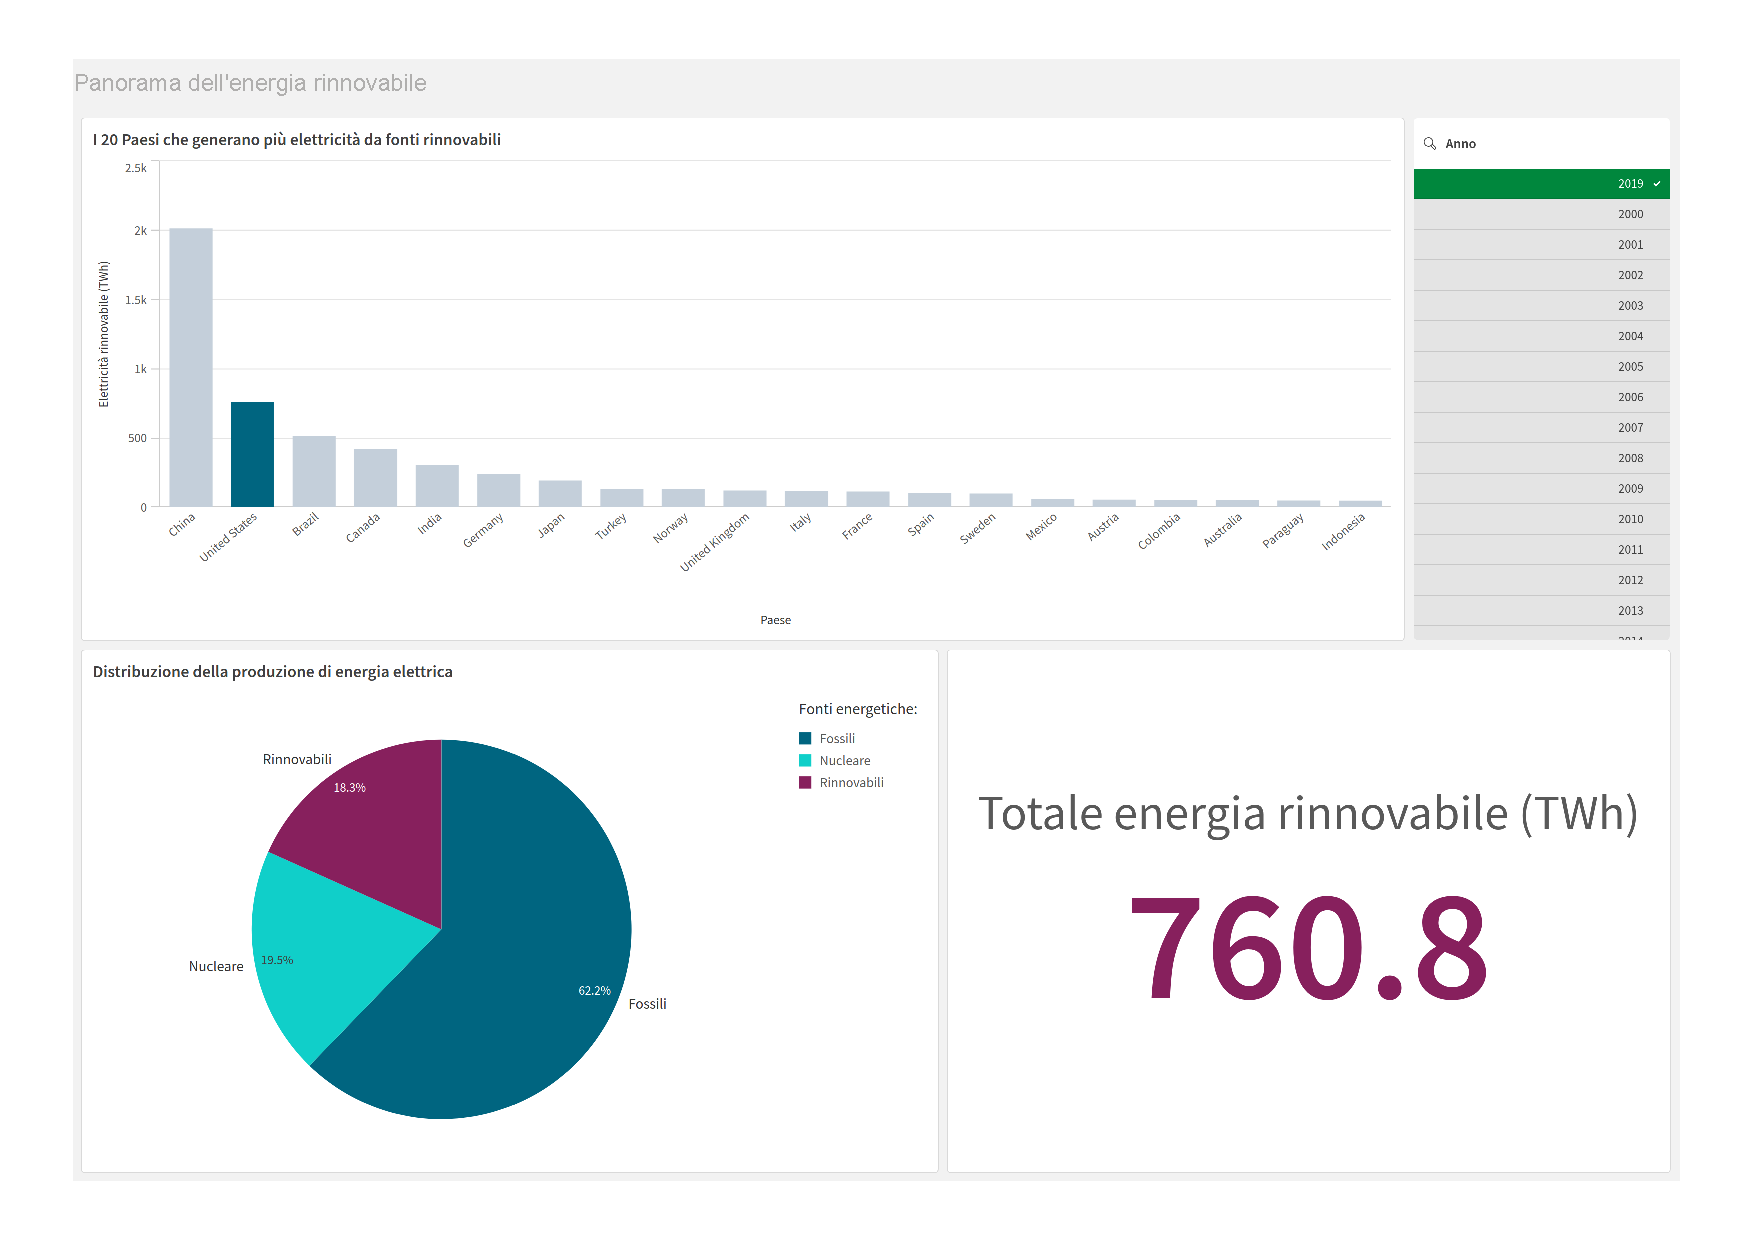
\includegraphics[width=0.50\textwidth]{capitolo_2/img2/5.5.3 Analisi USA 2019.pdf}}

    \caption{Analisi della produzione energetica di Cina e USA negli anni 2000, 2010 e 2019}
    \label{fig:analisi_cina_usa}
\end{figure}

Nel corso degli anni, la produzione di energie rinnovabili ha subito un'evoluzione significativa. Analizzando la situazione nel 2000, emerge come il Canada fosse il paese con la maggiore produzione di energia da fonti rinnovabili. Tuttavia, a livello globale, il contributo di queste fonti risultava ancora marginale rispetto alle fonti fossili, con un quantitativo complessivo pari a \texttt{2.56k}.  

A partire dal 2010, si osserva un cambiamento significativo nel panorama della produzione energetica: la Cina ha progressivamente assunto un ruolo di primo piano nel settore delle energie rinnovabili, aumentando in modo considerevole la propria capacità produttiva. Questo trend ha continuato a consolidarsi nel corso del tempo, come dimostrano i dati relativi al 2020, anno in cui la quantità di energia rinnovabile prodotta ha raggiunto \texttt{6.55k}.  


Nonostante la crescita costante delle fonti rinnovabili, le fonti fossili continuano a rappresentare la principale risorsa energetica a livello globale, mantenendo un ruolo predominante nel panorama energetico mondiale. Questo evidenzia come, sebbene la transizione energetica sia in atto, il processo di riduzione della dipendenza dai combustibili fossili richieda ancora tempo e investimenti significativi.

Questi risultati appaiono in apparente contrasto con le analisi presentate nella Sezione \ref{Sezione_4}, dove la Cina è stata identificata come il paese con i livelli più elevati di emissioni di CO\textsubscript{2}.

La Dashboard offre inoltre la possibilità di selezionare specifici stati su cui focalizzarsi, semplicemente cliccando sulle barre dell'istogramma corrispondente. In questo modo, l'utente può visualizzare in maniera interattiva i dati relativi a uno o più paesi di interesse. Nella Figura \ref{fig:analisi_cina_usa}, sono illustrate le analisi condotte per gli anni 2000, 2010 e 2019, con un particolare riferimento alle dinamiche energetiche degli Stati Uniti e della Cina. Queste immagini forniscono una panoramica dettagliata delle variazioni nella produzione e nell'uso delle risorse energetiche nei due paesi nel corso del tempo.
È importante osservare come, in questi paesi, si sia registrato un notevole aumento nell'adozione di energie rinnovabili, con una particolare espansione dell'uso del nucleare, specialmente negli Stati Uniti. Questi sviluppi sono il risultato di una serie di investimenti significativi, spesso sostenuti e promossi da politiche governative mirate a diversificare il panorama energetico e a ridurre la dipendenza dalle fonti fossili che storicamente ha costituito la principale risorsa energetica.


